\lhead{\begin{tikzpicture}[remember picture, overlay]
    \node [anchor=100,inner sep=0] (imagenIZQUIERDA) at (current page header area.north){
\includegraphics[width=18cm]{img/Encabezado.PNG}};
    \end{tikzpicture}}
    \rhead{Ángeles-Hurtado}
    \rfoot{\begin{tikzpicture}[remember picture, overlay]
    \node [anchor=140,inner sep=0] (imagenDERECHA) at (current page footer area.south){
\includegraphics[width=18cm]{img/Foot.PNG}};
    \end{tikzpicture}}
    %----------------------------------------------------------------------------------------
    \lfoot{ \thepage}
    % \renewcommand{\labelenumi}{\alph{enumi}.)} 
    %----------------------------------------------------------------------------------------
    %----------------------------------------------------------------------------------------
    %	TITLE SECTION
    %----------------------------------------------------------------------------------------
    
    \setlength{\droptitle}{-5\baselineskip} % Move the title up
    \title{\textbf{Estudio de tiempos y movimientos en el ensamble de un circuito electrónico utilizando diferentes métodos para su optimización }} % Article title
    
     \author{ 
     \textsc{Sanchez Nava Edwin Ernesto}\\ 
    %  Afiliación:
     \texttt{ Instituto Tecnológico de Querétaro} \\ 
     \texttt{Tecnológico Nacional de México } \\ 
     \texttt{Querétaro, México}\\ 
     \texttt{l22140867@queretaro.tecnm.mx} 
     \and 
     \textsc{Ángeles-Hurtado, Luis Alberto}\\ 
    %  Afiliación:
     \texttt{ Instituto Tecnológico de Querétaro } \\ 
     \texttt{ Tecnológico Nacional de México } \\ 
     \texttt{Querétaro, México}\\ 
     \texttt{alb3rt0.ah@gmail.com} 
    }
    
    
    %----------------------------------------------------------------------------------------
    
    % \begin{document}
    
    % Print the title
    \maketitle
    \thispagestyle{fancy}
    
    %----------------------------------------------------------------------------------------
    %	ARTICLE CONTENTS
    %----------------------------------------------------------------------------------------
    
    % \section*{Resumen}
    % \textit{Palabras clave:}
    % El resumen (ancho de página) deberá contener entre 100 y 200 palabras tipo Adobe Devangari 11 puntos.
    
    \begin{abstract}
    \noindent 
    El resumen (ancho de página) deberá contener entre 100 y 200 palabras tipo Adobe Devangari 11 puntos.
    
    \end{abstract}
    % 
    % 
    \textbf{\textit{Palabras clave}}: {First keyword should be the corresponding to the research area according with the authors guide. Maximum of 6 keywords.}
    % \keywords{First keyword should be the corresponding to the research area according with the authors guide. Maximum of 6 keywords.}
    
    \section{Introducción}
    
    % \begin{itemize}
    %     \item Se debe exponer de manera concreta y en lenguaje sencillo : el tema, o lo(s) objeto (s) de estudio. 
    %     \item Se deben de mencionar las metodologías más usadas muy brevemente. 
    %     \item Se debe de señalar el avance en los últimos años.
    %     \item Al final se debe hacer alusión al o lo(s) objetivos del proyecto de investigación.
    %     \item Debe de tener Referencias científicas, URL, tesis, etc.
    % \end{itemize}
    % Define estudio de tiempos y movimientos
     El estudio de tiempos y movimientos es una disciplina fundamental en la ingeniería industrial, que se enfoca en analizar y mejorar la eficiencia de los procesos productivos. En el contexto del ensamble de circuitos electrónicos, este estudio cobra una relevancia particular debido a la naturaleza precisa y delicada de las operaciones involucradas.
     Dicho estudio se implementara en el ensamble de un circuito electrónico, los circuitos electrónicos implica la manipulación de componentes pequeños y delicados, así como la realización de conexiones precisas. Todo esto optimizando los movimientos y tiempos requeridos en la elaboración del circuito, la optimización es buscar la mejor manera de realizar una actividad.\cite{RAE}  
     Otro método a utilizar en este proyecto es el método de tiempos predeterminados que se puede definir como el conjunto de reglas o métodos para determinar con anticipación la secuencia de sucesos. En este sentido, el presente estudio se propone explorar diferentes métodos y técnicas para analizar, medir y mejorar los tiempos y movimientos en el ensamble de circuitos electrónicos \cite{sistema-tiempos-predeterminados}.
    % 
    % 
    \section{Justificación}
    
    % \begin{itemize}
    %     \item Se debe de describir lo que se requiere, lo que se necesita o lo que se demanda en la actualidad con un enfoque global pero terminar con menciones a temas locales o nacionales.
    %     \item Debe de tener Referencias científicas, URL, tesis, etc.
    % \end{itemize}
    % 
    % Se debe de describir lo que se requiere, lo que se necesita o lo que se demanda en la actualidad con un enfoque global pero terminar con menciones a temas locales o nacionales.
    % 
    La manufactura a lo largo de las revoluciones industriales ha tenido grandes avances. Actualmente existen diversos tipos de manufactura que a lo largo del tiempo siguen evolucionando.
        Para ser más concretos podemos afirmar que existen por lo menos ocho diferentes tipos de manufactura y que se aplican a diversas industrias
        México se encuentra en el puesto número siete con 314,701 millones de dolares en el año 2020.
        Basándonos en la gráfica que proporciona el banco mundial México se encuentra en crecimiento y desarrollo.
    % Cuantas empresas de manufactura existen en Querétaro?
        Existen por lo menos 7,649 empresas dedicadas a la manufactura.
        El estudio de tiempos y movimientos en el ensamble de circuitos electrónicos es crucial debido a varios factores clave que afectan tanto la eficiencia operativa como la calidad del producto final. A continuación se presentan algunas razones que respaldan la necesidad de llevar a cabo este estudio utilizando diferentes métodos para su optimización:
        \begin{itemize}
            \item Optimización de recursos: El ensamble de circuitos electrónicos implica el uso de recursos costosos y delicados, como componentes electrónicos y equipos especializados. Optimizar los tiempos y movimientos ayuda a maximizar la utilización de estos recursos, minimizando el desperdicio y reduciendo los costos de producción.
            \item  Al identificar y eliminar actividades innecesarias o redundantes, así como optimizar los procesos de ensamble, se puede aumentar la productividad de la línea de producción. Esto se traduce en una mayor cantidad de circuitos electrónicos ensamblados en un período de tiempo dado, lo que mejora la capacidad de respuesta ante la demanda del mercado.
            \item Calidad del producto: Los tiempos y movimientos ineficientes pueden contribuir a errores de ensamble, mal funcionamiento de los circuitos electrónicos y defectos en el producto final. Al optimizar estos aspectos, se reduce la probabilidad de errores y se mejora la calidad del producto, lo que conduce a una mayor satisfacción del cliente y una reputación positiva de la marca.
            \item Ergonomía y seguridad laboral: Un estudio detallado de los movimientos realizados por los operarios en el ensamble de circuitos electrónicos permite identificar y corregir posturas incómodas o movimientos repetitivos que pueden causar fatiga o lesiones laborales. Mejorar la ergonomía en el lugar de trabajo no solo aumenta el bienestar de los empleados, sino que también puede aumentar la eficiencia y la precisión en las tareas realizadas.
            \item  En un mercado globalizado y altamente competitivo, las empresas que pueden producir circuitos electrónicos de manera más eficiente y con una calidad superior tienen una ventaja significativa. El estudio de tiempos y movimientos, junto con su optimización, ayuda a las empresas a mejorar su competitividad al reducir costos, mejorar la calidad y aumentar la capacidad de respuesta a las demandas del mercado.
        \end{itemize}
    
        %La optimización de procesos de ensamble es fundamental para mejorar la eficiencia y la productividad en entornos industriales. Mediante un estudio de tiempos detallado, podemos identificar áreas de oportunidad para reducir los tiempos de producción, minimizar los tiempos muertos y mejorar la calidad del producto final. Este proyecto tiene como objetivo principal aplicar técnicas de ingeniería industrial para analizar y mejorar el proceso de ensamble, lo que resultará en una reducción de costos, un aumento en la producción y una mayor satisfacción del cliente. Al entender mejor cómo se lleva a cabo el ensamble y dónde se pueden realizar mejoras, podemos optimizar el flujo de trabajo, eliminar cuellos de botella y aumentar la eficiencia operativa. En última instancia, este proyecto contribuirá significativamente a la competitividad y rentabilidad de nuestra empresa en un mercado cada vez más exigente y competitivo.
    
        \begin{itemize}
           \item Se debe de describir lo que se requiere, lo que se necesita o lo que se demanda en la actualidad con un enfoque global pero terminar con menciones a temas locales o nacionales.
           % \item Debe de tener Referencias científicas, URL, tesis, etc.
        \end{itemize}
        % 
        % 
    \section{Descripción del problema}
    
    % \begin{itemize}
    %     \item Se debe describir la desviación o diferencia del ``es'' con respecto al ``debe ser''.
    %     \item Se debe hacer alusión a la incógnita científica*.
    %     \item Debe de tener Referencias científicas, URL, tesis, etc.
    % \end{itemize}
    % \textbf{*La incógnita científica es el elemento cuya solución incrementa el conocimiento científico.}
    % 
    % 
    % ``es''
    La educación y el desarrollo tecnológico contribuyen al crecimiento del país por lo que invertir en todos los sectores de la industria mejora los ingresos de las familias mexicanas y se tiene una mejor calidad de vida.
    % ``debe ser''
    Los estudiantes del tecnológico de México deberían desarrollar habilidades de las ultimas tendencias tecnológicas para ser competitivos a nivel mundial.
    % 
    La falta de tiempo a la materia y la falta de habilidades computacionales, de investigación, trabajo en equipo y trabajo autónomo limitan el aprendizaje de los alumnos.
    % 
    El problema del estudio de tiempos y movimientos en el ensamble de circuitos electrónicos abarca una serie de desafíos complejos que pueden afectar tanto la eficiencia operativa como la calidad del producto final.
    En resumen, el problema del estudio de tiempos y movimientos en el ensamble de circuitos electrónicos abarca una serie de desafíos que afectan la eficiencia, la calidad, la seguridad laboral y la rentabilidad del proceso. La aplicación de diferentes métodos de optimización es fundamental para abordar estos desafíos de manera efectiva y promover la excelencia en la producción de circuitos electrónicos.
    % 
    \section{Fundamentación teórica}
    
     La fundamentación teórica del estudio de tiempos y movimientos en el ensamble de un circuito electrónico se basa en varios principios y conceptos fundamentales de la ingeniería industrial y la gestión de operaciones. Aquí hay una descripción de algunos de los aspectos teóricos clave:
        \begin{itemize}
            \item Análisis de tiempos: Este método implica medir y registrar el tiempo requerido para completar cada tarea individual en el proceso de ensamble. Se basa en la idea de que entender cómo se distribuye el tiempo entre las diferentes actividades permite identificar oportunidades de mejora y eliminar actividades innecesarias o redundantes. El análisis de tiempos proporciona una base cuantitativa para evaluar la eficiencia del proceso y diseñar intervenciones de mejora.
            \item Cronometraje de movimientos: Este enfoque se centra en analizar y mejorar los movimientos físicos realizados por los trabajadores durante el ensamble de circuitos electrónicos. Se basa en los principios de ergonomía y biomecánica para identificar movimientos ineficientes, repetitivos o que puedan causar fatiga o lesiones. Al optimizar los movimientos, se puede mejorar la eficiencia del proceso y reducir el riesgo de lesiones laborales.
            \item Estudio de métodos: Este método implica analizar y comparar diferentes métodos o técnicas utilizadas para realizar una tarea específica en el ensamble de circuitos electrónicos. Se busca identificar el método más eficiente que permita completar la tarea de manera rápida, precisa y segura. El estudio de métodos puede involucrar la evaluación de herramientas, equipos, diseños de estaciones de trabajo y procedimientos de trabajo.
        \end{itemize}
        % 
        % 
    % Cuales son las revoluciones industriales que ha vivido la humanidad?
    % A lo largo de la historia del hombre las técnicas manuales para elaborar herramientas y mejorar la caza y la calidad de vida fueron fundamentales para la supervivencia.
    % La revolución industrial han cambiado las fuentes de energía básicas y los medios de comunicación para desplazar mercancías, personas e información.
    % 
    % 
    \section{Hipótesis}
    
    % Es la suposición con fundamento científico relativa a la solución del problema, necesidad o de cómo se aprovecha la oportunidad con la incógnita científica y se fundamenta con: 1. Una suposición (en afirmativo o negativo) y ésta deberá vincularse con:
    % 2. La fundamentación científica que deberá ser precisa 3. Una entidad de comparación para probar la suposición y
    % 4. La variable con que se califica o cuantifica la comparación o se prueba la hipótesis.
    % 
    % 
    Desarrollar un proyecto integrador en la materia de estudio del trabajo II implementando todos los temas vistos en la clase incrementara las habilidades del estudiante logrando plantear nuevos proyectos desde cero al determinar el tiempo estándar en el ensamble de un circuito electrónico.
    Aquí hay algunas hipótesis que podrían plantearse en el contexto del estudio de tiempos y movimientos en el ensamble de un circuito electrónico:
        \begin{itemize}
            \item  Se hipotetiza que la aplicación de técnicas de análisis de tiempos y movimientos, junto con métodos de optimización, permitirá reducir significativamente los tiempos de ciclo en el ensamble de circuitos electrónicos, mejorando así la eficiencia del proceso.
            \item Se plantea que al optimizar los movimientos y métodos de ensamble, se reducirán los errores y defectos en el producto final, lo que resultará en una mejora general en la calidad de los circuitos electrónicos ensamblados.
            \item Se plantea que al analizar y optimizar los movimientos realizados por los trabajadores durante el ensamble de circuitos electrónicos, se mejorará la ergonomía de las estaciones de trabajo, reduciendo la fatiga y el riesgo de lesiones laborales.
        \end{itemize}
        Estas hipótesis proporcionan un marco inicial para el estudio y la investigación sobre la optimización del ensamble de circuitos electrónicos a través del análisis de tiempos y movimientos, y pueden servir como base para la formulación de objetivos y la evaluación de resultados.
    % 
    % 
    % \begin{itemize}
    %     \item Se debe de identificar claramente la suposición científica
    %     \item Se debe de identificar claramente el fundamento científico
    %     \item Se debe identificar claramente la variable de respuesta
    %     \item Se debe identifican claramente las realidades o modelos contrastantes
    %     \item Se debe de establecer las variables asociadas, explicativas o que tienen relación funcional con la variable de respuesta
    % \end{itemize}
    % 
    % 
    \section{Objetivo}
    % Precisar la acción necesaria para probar la hipótesis. Dicha acción se establece mediante el uso de verbos activos y en infinitivo.
    % 
    % 
    % \begin{itemize}
    %     \item Se debe establecer que se pretende probar la hipótesis
    % \end{itemize}
    % 
    % 
    El alumno diseñará, mejorará e integrará sistemas productivos de bienes y servicios aplicando tecnologías para su optimización.
    Diseñará, implementará y mejorará sistemas de trabajo para elevar la productividad.
    En un plazo menor a seis meses y se plasmara en un proyecto integrador.
    % 
    El objetivo principal del estudio de tiempos y movimientos en el ensamble de un circuito electrónico es mejorar la eficiencia, la calidad y la seguridad del proceso de producción. Para lograr este objetivo, se pueden establecer los siguientes objetivos específicos:
    % 
    \subsection{Objetivos específicos}
    
    % \begin{itemize}
    %     \item Se debe establecer como un conjunto de acciones comunes para lograr el objetivo general
    %     \item Se debe establecer como etapas para lograr el objetivo general
    % \end{itemize}
    
    % Son actividades orientadas al cumplimiento del objetivo general. Se establecen con verbos activos en infinitivo. Son parte de la acción encaminada a probar la hipótesis. Éstos deben ser precisos, y en lo posible evitar aspectos metodológicos.
    % 
    % 
    \begin{itemize}
            \item Reducir los tiempos de ciclo: Mediante la identificación y eliminación de actividades innecesarias, así como la optimización de los movimientos y métodos de ensamble, se busca reducir el tiempo total requerido para ensamblar un circuito electrónico, aumentando así la productividad y la capacidad de respuesta del proceso.
            \item Mejorar la calidad del producto: Al optimizar los tiempos y movimientos, se busca reducir la probabilidad de errores y defectos en el producto final. Esto se logra mediante la estandarización de procedimientos, la mejora de la precisión en el ensamble y la implementación de controles de calidad efectivos.
            \item Optimizar el uso de recursos: Se pretende utilizar de manera más eficiente los recursos disponibles, como el tiempo de trabajo, el espacio de trabajo, los equipos y los materiales. Esto implica minimizar el desperdicio y maximizar la utilización de los recursos para reducir los costos de producción y aumentar la rentabilidad.
            \item Promover la mejora continua: El estudio de tiempos y movimientos proporciona una base sólida para la identificación de oportunidades de mejora y la implementación de cambios efectivos en el proceso de ensamble de circuitos electrónicos. Se busca fomentar una cultura de mejora continua, donde se busque constantemente optimizar el proceso y adaptarse a los cambios en el entorno operativo. 
    
        \end{itemize}
    %
    % 
    c\section{Metodología}
    
    Este trabajo de investigación se llevó a cabo mediante la observación y el análisis estadístico. La recolección de datos y el estudio se realizaron en Querétaro, específicamente en las instalaciones de ITQ. El período de experimentación abarcó desde febrero hasta mayo de 2024.
    Se ejemplificó el ensamblaje de una tarjeta electrónica mediante el uso de software de diseño asistido por computadora. Se definió la estructura de todos los niveles, se establecieron los límites de potencia y control necesarios para desarrollar la arquitectura requerida y, finalmente, se seleccionó la opción óptima para su implementación.
    En la primera fase experimental, se capturaron dos muestras continuas utilizando una cámara de vídeo. Posteriormente, se emplearon diversas metodologías para determinar el tiempo ciclo y el tiempo estándar.
    % 
    % 
    \subsection{Desarrollo de la guía de plan de Emergencia}
    
    El Plan de Emergencia: Documento que describe los lineamientos a seguir, la organización y los mecanismos, que indican la manera de enfrentar una situación de emergencia o desastre tanto en lo general como en lo particular, así como la utilización viable de los recursos humanos y materiales con los que se cuenta.El objetivo de este documento es brindar una guía sobre los principales aspectos para la elaboración de un plan de emergencia en centros de trabajo Este modelo deberá ser adaptado de acuerdo a las características de cada lugar de trabajo.\cite{romero1993guia}
    % 
    % 
    \subsection{Análisis de los métodos, materiales, herramientas e instalación utilizada en la ejecución del ensamble de un circuito electrónico}
    
    \subsubsection{Planeación}
    
    Asegúrate de conocer siempre tu objetivo.
    Asegúrate de contar con los documentos (formatos, procedimientos, etc).
    % 
    % 
    \subsubsection{5's}
    
    Consiste en tener un lugar de trabajo
    más ordenado, limpio y organizado que
    permite elevar la productividad y
    eficiencia en una empresa, haciéndolo de manera permanente.
    Las etapas son las siguientes: Seleccionar, Ordenar, Limpiar, Estandarizar, y Sostener.
    % 
    % 
    \subsubsection{Desarrollo del sistema de tiempos predeterminado}
    \begin{figure}[H]
        \centering
        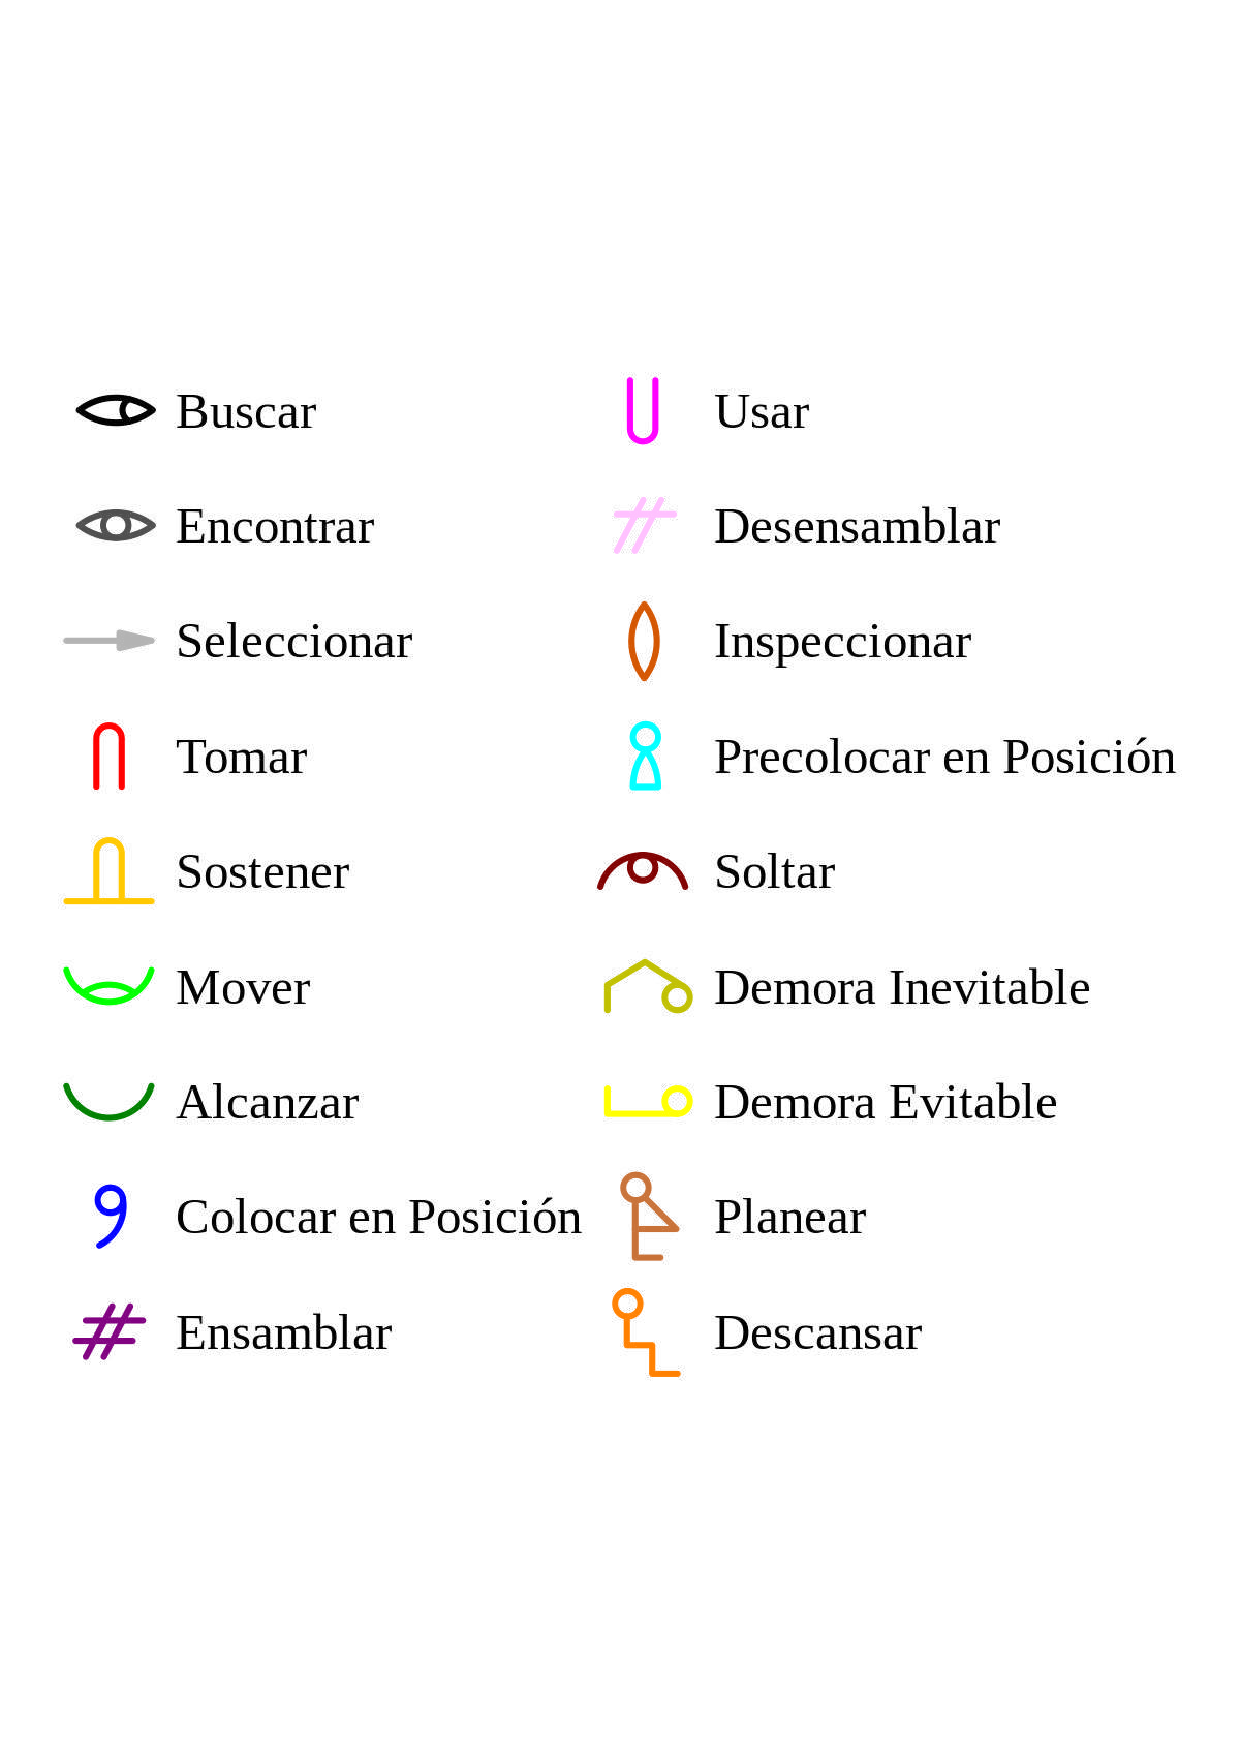
\includegraphics[scale=0.185]{30/img/therblig.pdf}
        \caption{Los therblig}
        % \label{fig:my_label}
    \end{figure}
    % 
    % 
    \subsubsection{Desarrollo del muestreo del trabajo}
    
    % 
    % 
    \subsubsection{Corrección por balanceo de procesos}
    % 
    % 
    \subsubsection{Datos estándar continuos y discretos}
    % 
    % 
    
    % 
    % 
    
    % 
    % 
    \subsection{Diseño de la forma más económica de realizar el trabajo}
    
    % 
    % 
    \subsection{Normalización de los métodos, materiales, herramientas e instalaciones}
    
    % 
    % 
    \subsection{Determinación del tiempo estándar para que una persona competente realice el trabajo con marcha normal}
    El tiempo estándar para una operación se refiere al periodo requerido para que un trabajador promedio, completamente capacitado y entrenado, trabajando a una velocidad normal, complete la operación. Este tiempo se establece sumando el tiempo asignado a todos los elementos considerados en el estudio de tiempos, como se muestra en la tabla mencionada como \ref{fig:tabalatiempoestandar}.
    
    Para calcular el tiempo estándar, es crucial considerar los suplementos o márgenes aplicados durante el ensamblaje. Estos márgenes se dividen en dos categorías: suplementos constantes y suplementos variables o por fatiga. La distribución de estos márgenes, así como sus diferencias entre hombres y mujeres, se detalla en la tabla \ref{fig:tablasholguras}.
    
    Para calcular los márgenes utilizados en el ensamblaje del circuito, se debe consultar la tabla , que muestra el porcentaje de cada tipo de margen. Finalmente, se suman todos estos márgenes para obtener un valor total, el cual se incorpora en la tabla de tiempo estándar (\ref{fig:calculodeholguras}).
    
    Con todos los elementos necesarios completados en la tabla de tiempo estándar y siguiendo las operaciones indicadas, se puede obtener el tiempo estándar deseado.
    \begin{figure}[H]
        \centering
        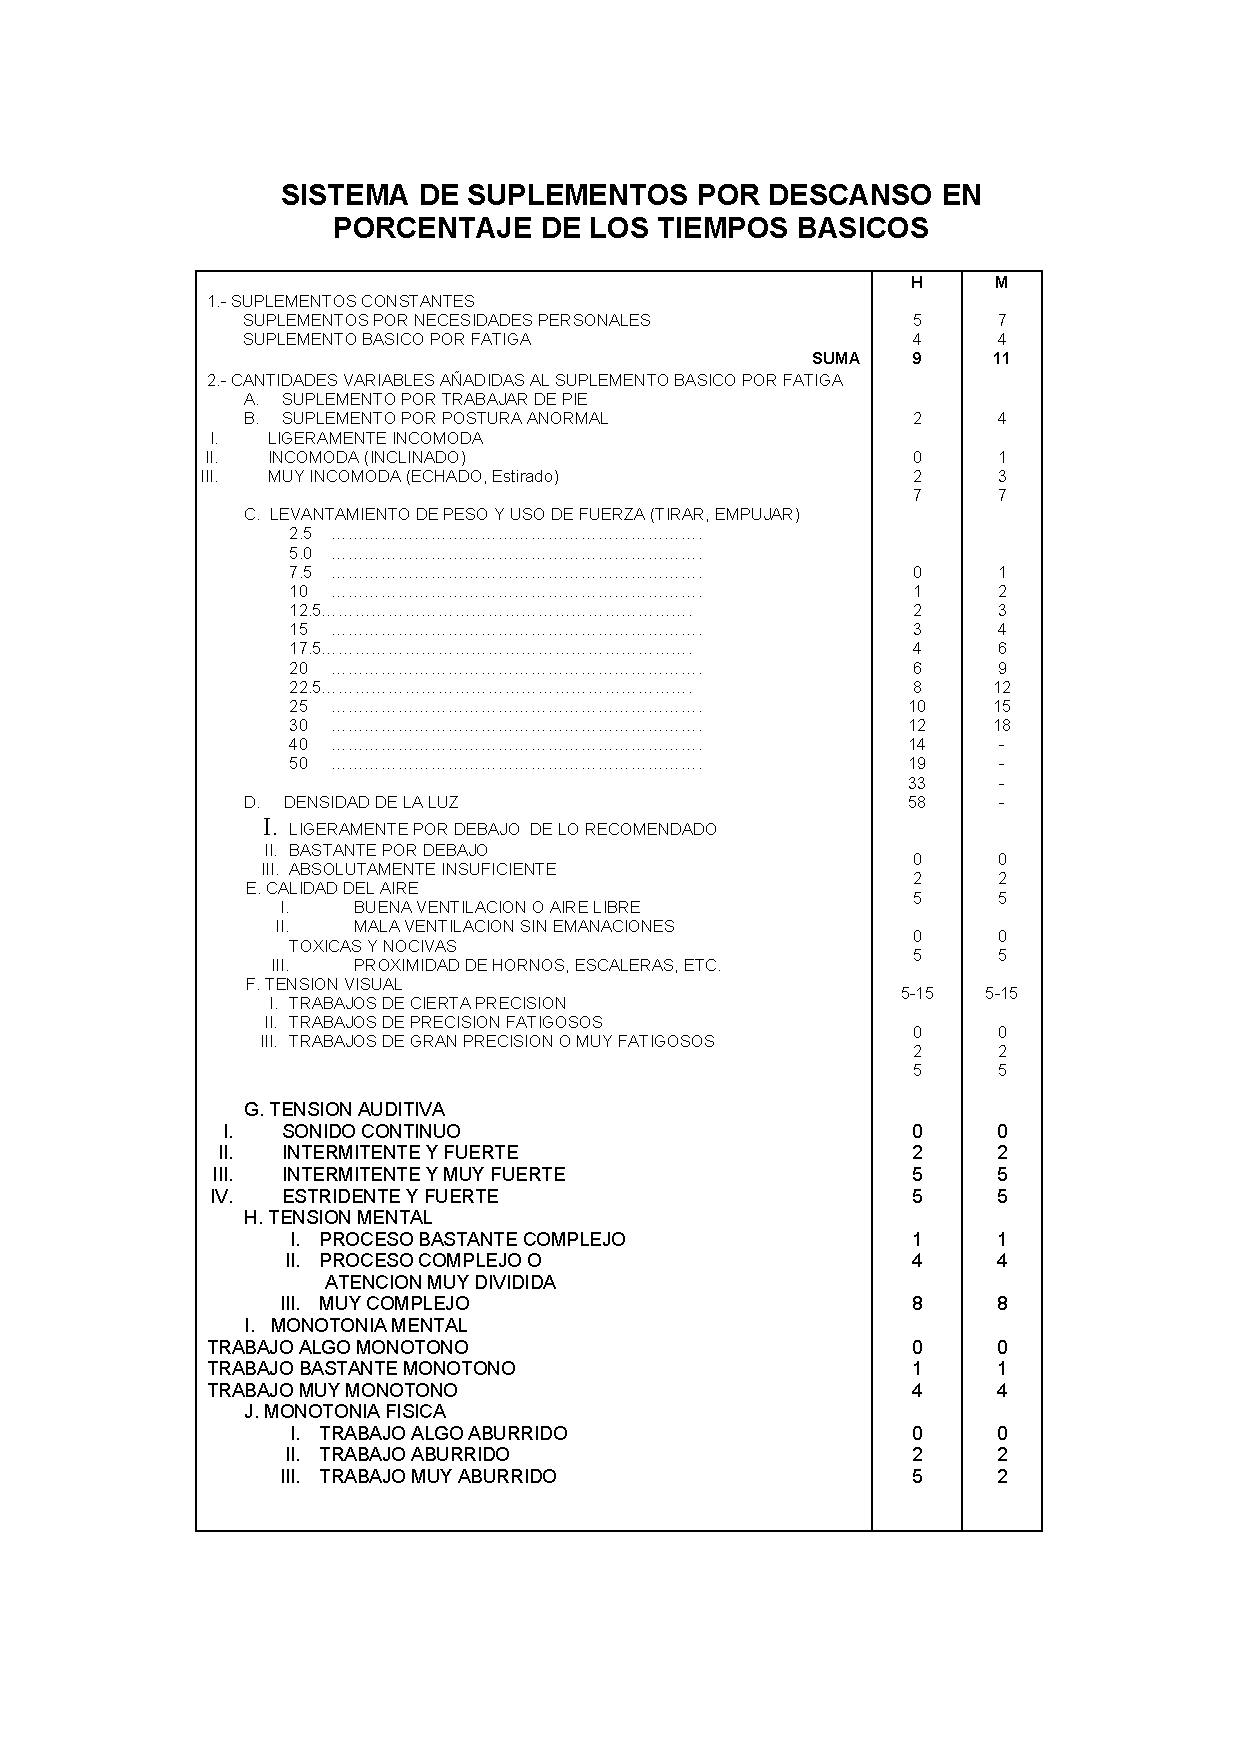
\includegraphics[scale=0.23]{30/img/tablaHolguras.pdf}
        \caption{Tablas de holguras}
        \label{fig:tablasholguras}
    \end{figure}
    \begin{figure}[H]
        \centering
        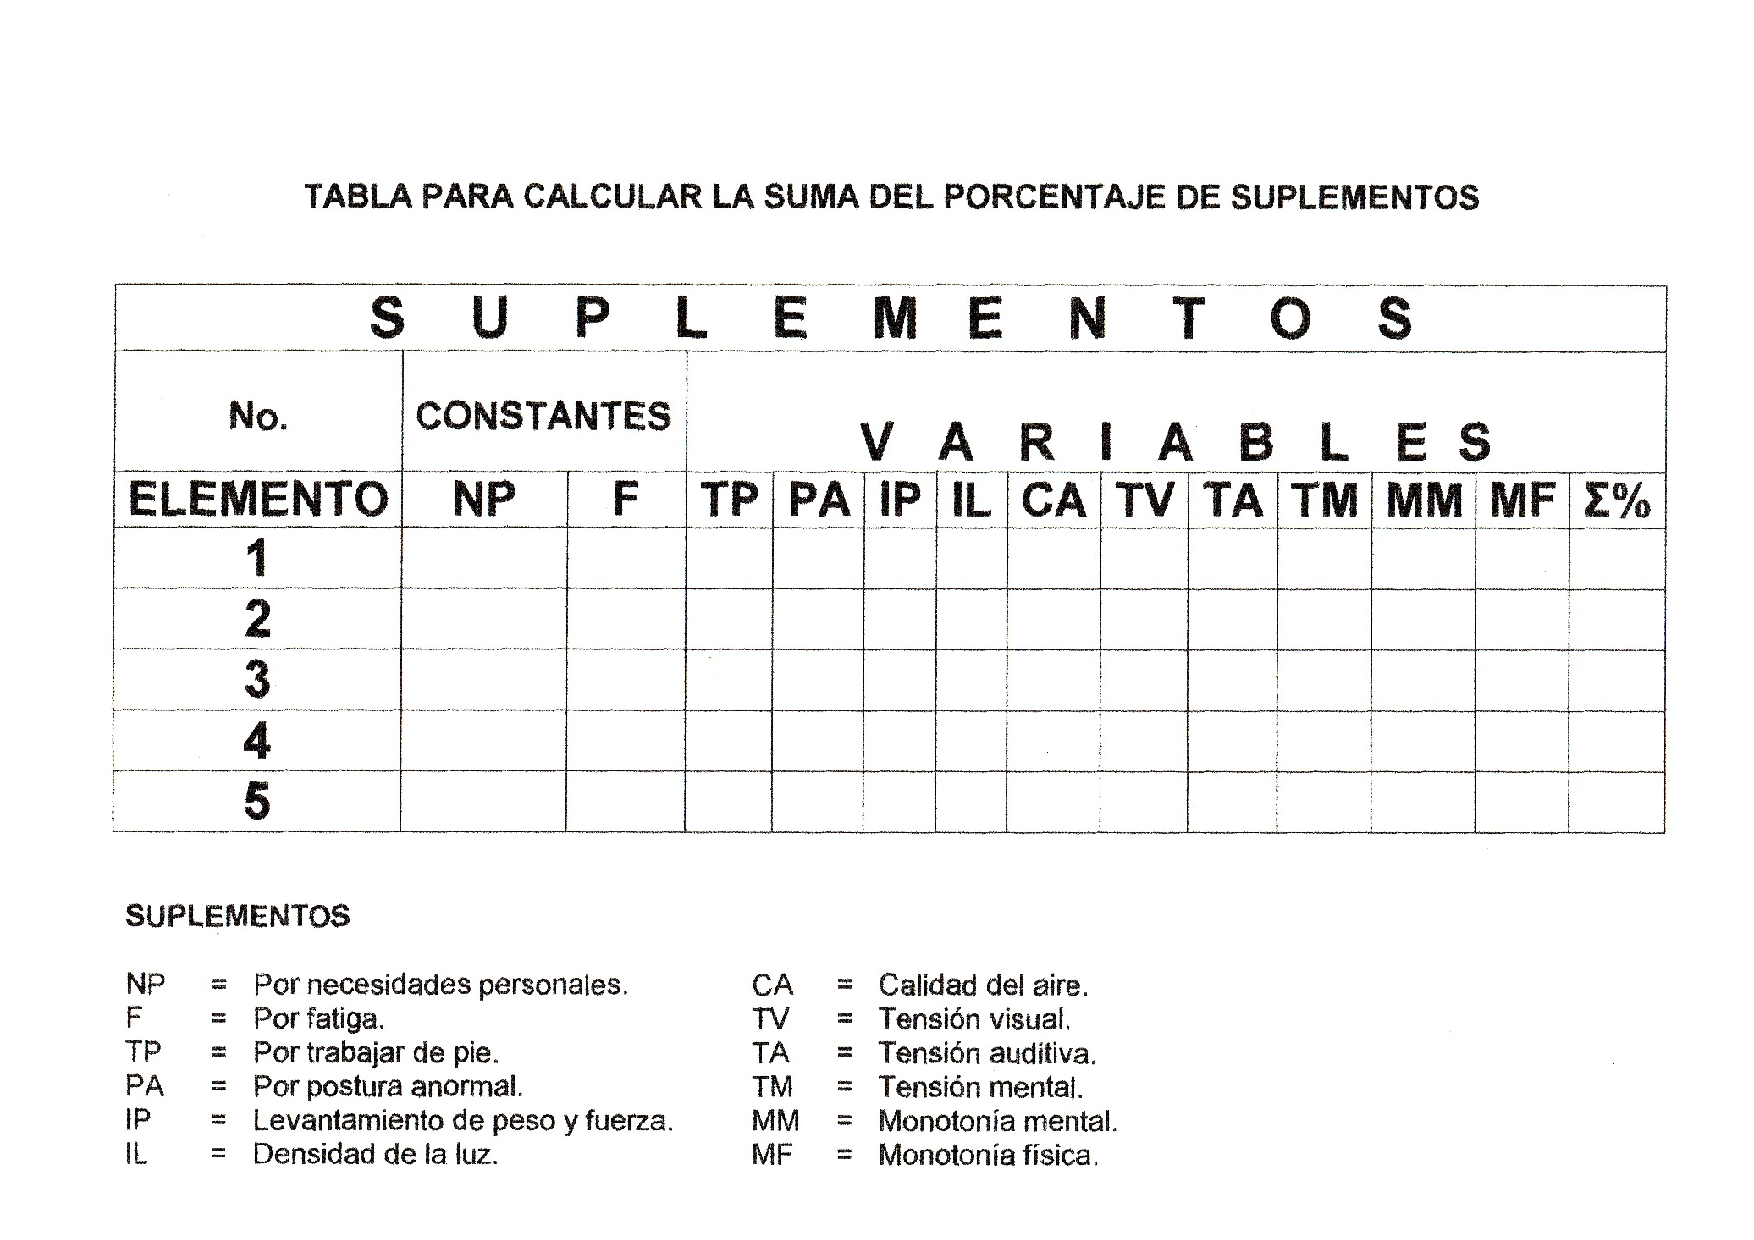
\includegraphics[scale=0.23]{30/img/tablaCalculoHolguras.pdf}
        \caption{Calculo de holguras}
        \label{fig:calculodeholguras}
    \end{figure}
    \begin{figure}[H]
        \centering
        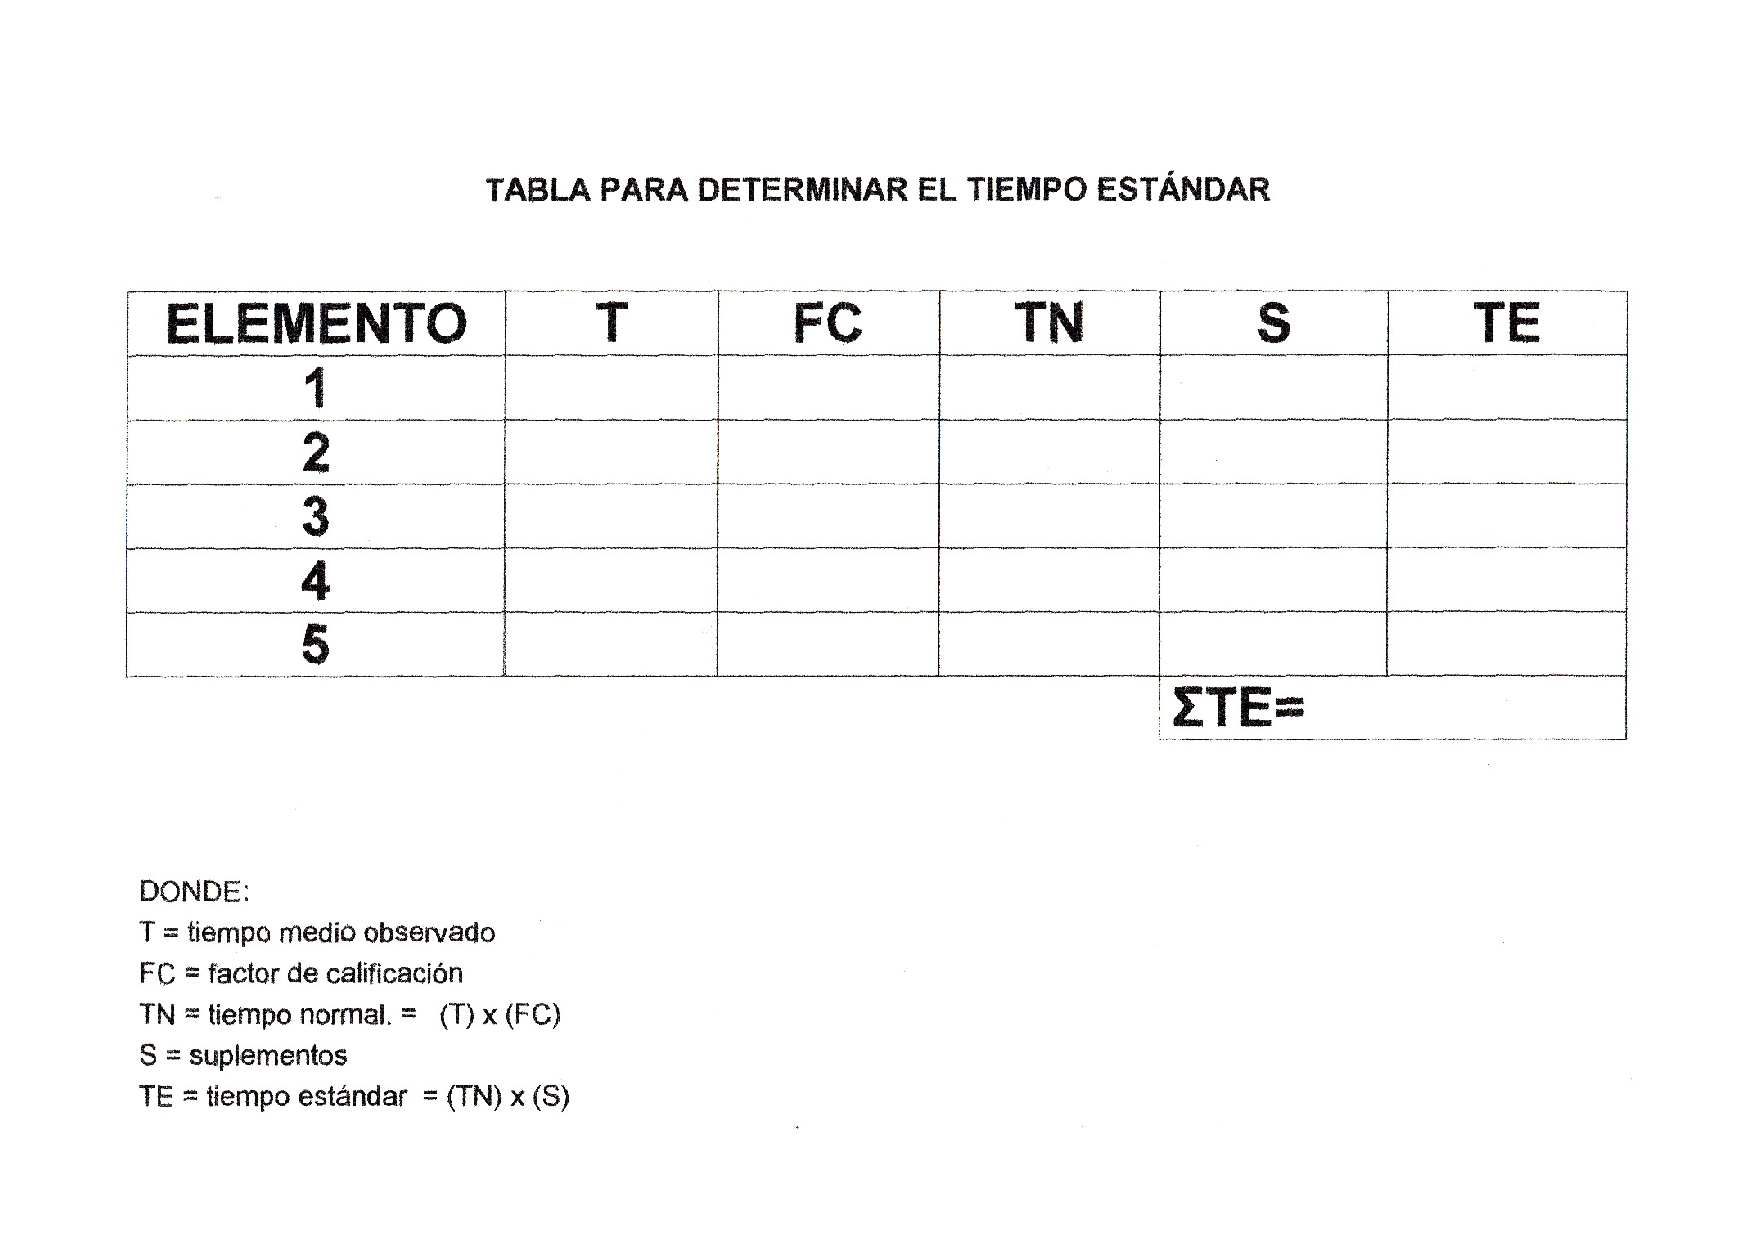
\includegraphics[scale=0.23]{30/img/tablaTiempoEstandar.pdf}
        \caption{Tablas de tiempo estandar}
        \label{fig:tabalatiempoestandar}
    \end{figure}
    % 
    % 
    % \subsection{Acrónimos y Abreviaciones}
    
    % Los acrónimos y abreviaciones deberán ser definidos únicamente la primera vez que aparecen en el texto, esto para que el lector entienda lo que significan.
    
    % \subsection{Ecuaciones}
    
    % Las ecuaciones son una excepción a las especificaciones prescritas de esta plantilla. 
    % Deberá determinar si su ecuación debe escribirse o no utilizando la fuente Adobe Devangari. 
    % Para crear ecuaciones multinivel, puede ser necesario tratar la ecuación como un gráfico e insertarla en el texto después de aplicar el estilo de la platilla.
    % Las ecuaciones serán enumeradas de manera consecutiva, y el número de ecuación, entre paréntesis, se colocan al ras de la derecha, utilizando una tabulación derecha.
    % 
    % \begin{equation}
    %     \label{eq1}
    %     x + y = z 
    % \end{equation}
    % 
    % Es importante asegurarse de que los símbolos de la ecuación sean definidos antes o inmediatamente después de la ecuación. Utilice “(1)”, en vez de “Eq. 1” al enumerar las ecuaciones, excepto al principio de una oración: “La ecuación (\ref{eq1}) es…”
    
    \section{Resultados y discusión}
    
    \subsection{Desarrollo de la guía de plan de Emergencia}
    
    Con esta guía, buscamos minimizar las emergencias de incendio y los riesgos de accidentes en el Instituto Tecnológico de Querétaro. Para lograrlo, se ofrecen capacitaciones anuales al personal, las cuales les permitirán tomar decisiones adecuadas en situaciones de emergencia, garantizando la seguridad de todas las personas dentro y fuera de la institución, así como la protección de las instalaciones
    Los datos generales del establecimiento se pueden resumir en la Figura \ref{fig:mapa-itq}.
    % 
    % 
    \begin{figure}[H]
        \centering
        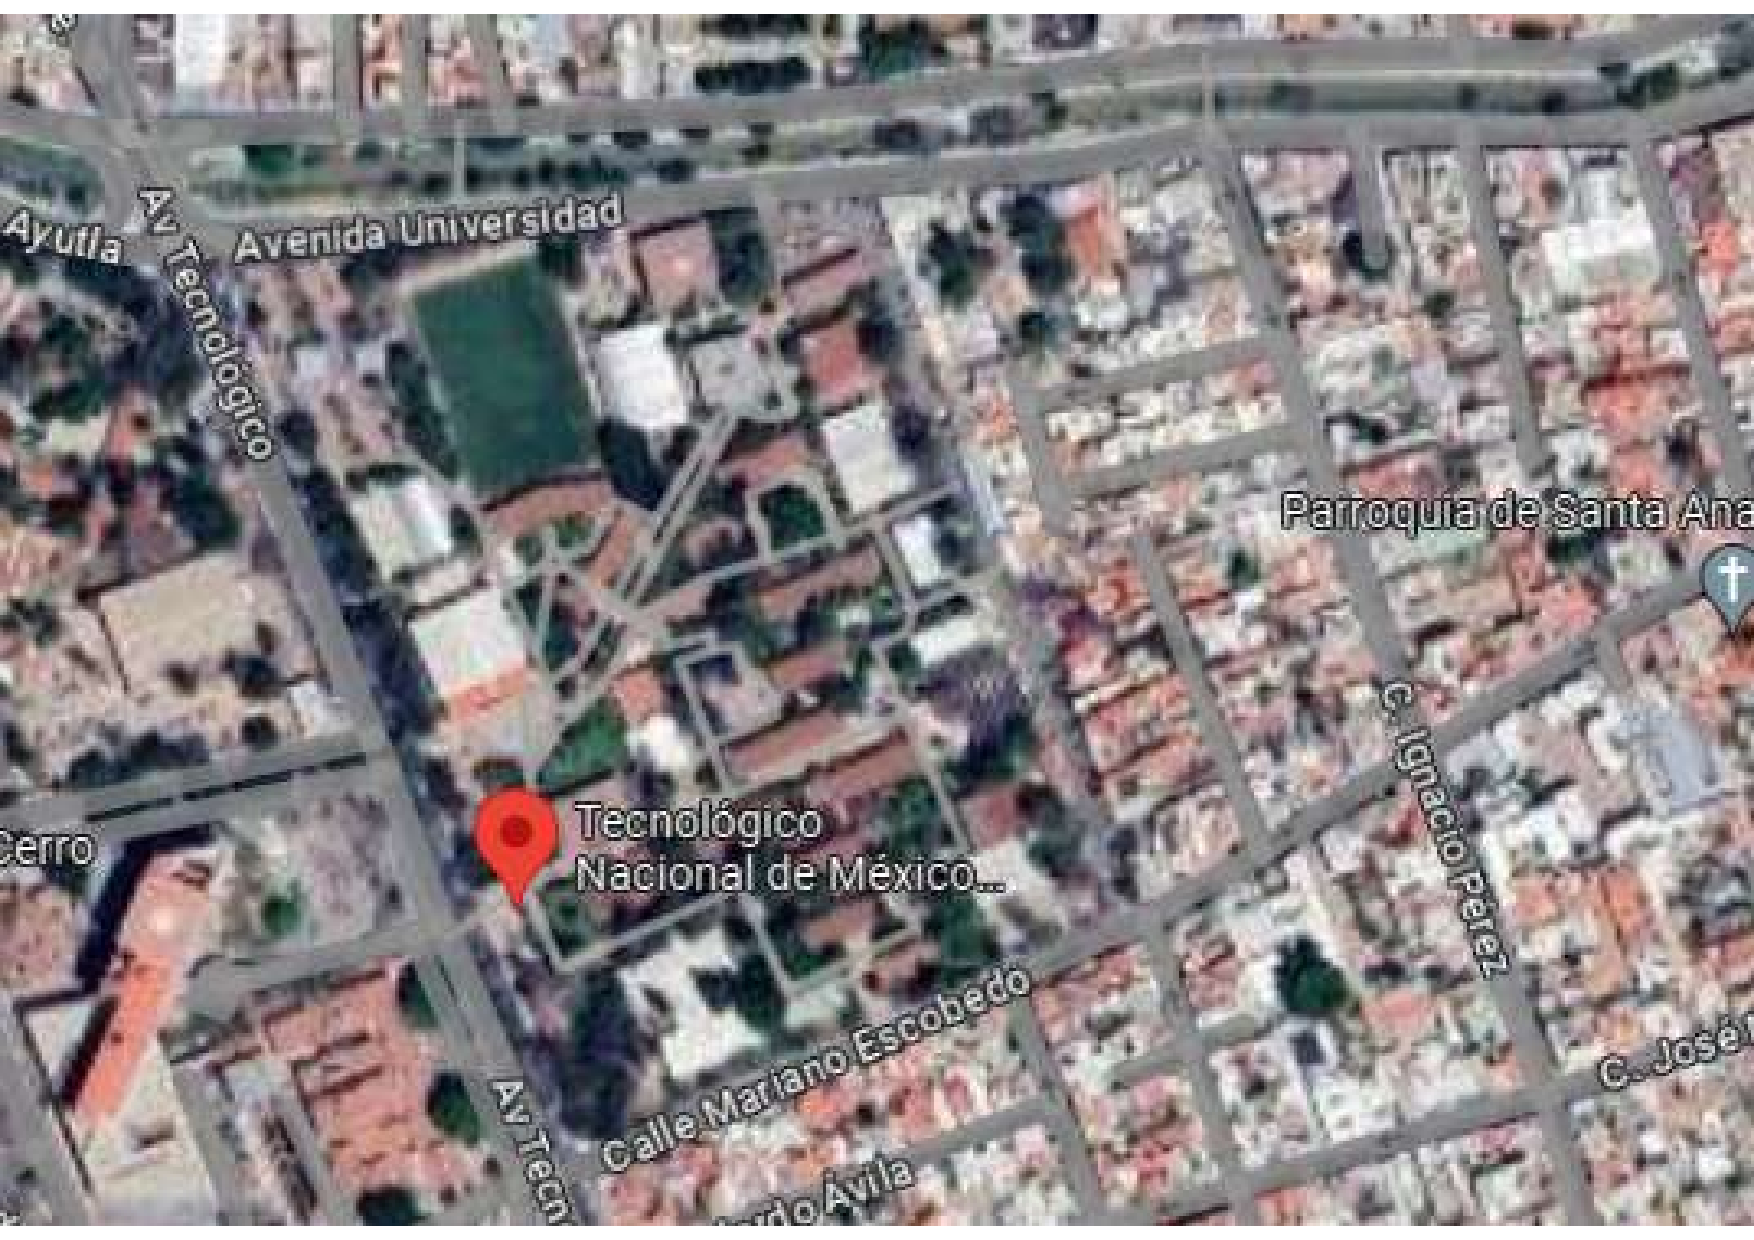
\includegraphics[scale=0.23]{30/img/Fotoescuela.pdf}
        \caption{Tecnológico Nacional de México, Instituto Tecnológico de Querétaro, Av Tecnológico S/N, Centro Histórico, Centro, 76000, Querétaro, Qro., 4422274400 Ext. 4423}
        \label{fig:mapa-itq}
    \end{figure}
    % 
    % 
    \subsubsection{Identificación del riesgo}
    
    Nos comprometemos a ejecutar un programa de prevención de riesgos tanto interna como externamente todos los días. Además, buscamos obtener comentarios tanto de nuestros clientes internos como externos sobre los riesgos que enfrentamos en nuestras actividades habituales. Animamos a todo el equipo a involucrarse activamente en este proceso. Cada riesgo, ya sea interno o externo, será evaluado y categorizado según su nivel de importancia. Esto nos ayudará a priorizar nuestras acciones y tomar las medidas necesarias para abordarlos.
    % 
    % 
    \begin{figure}[H]
        \centering
        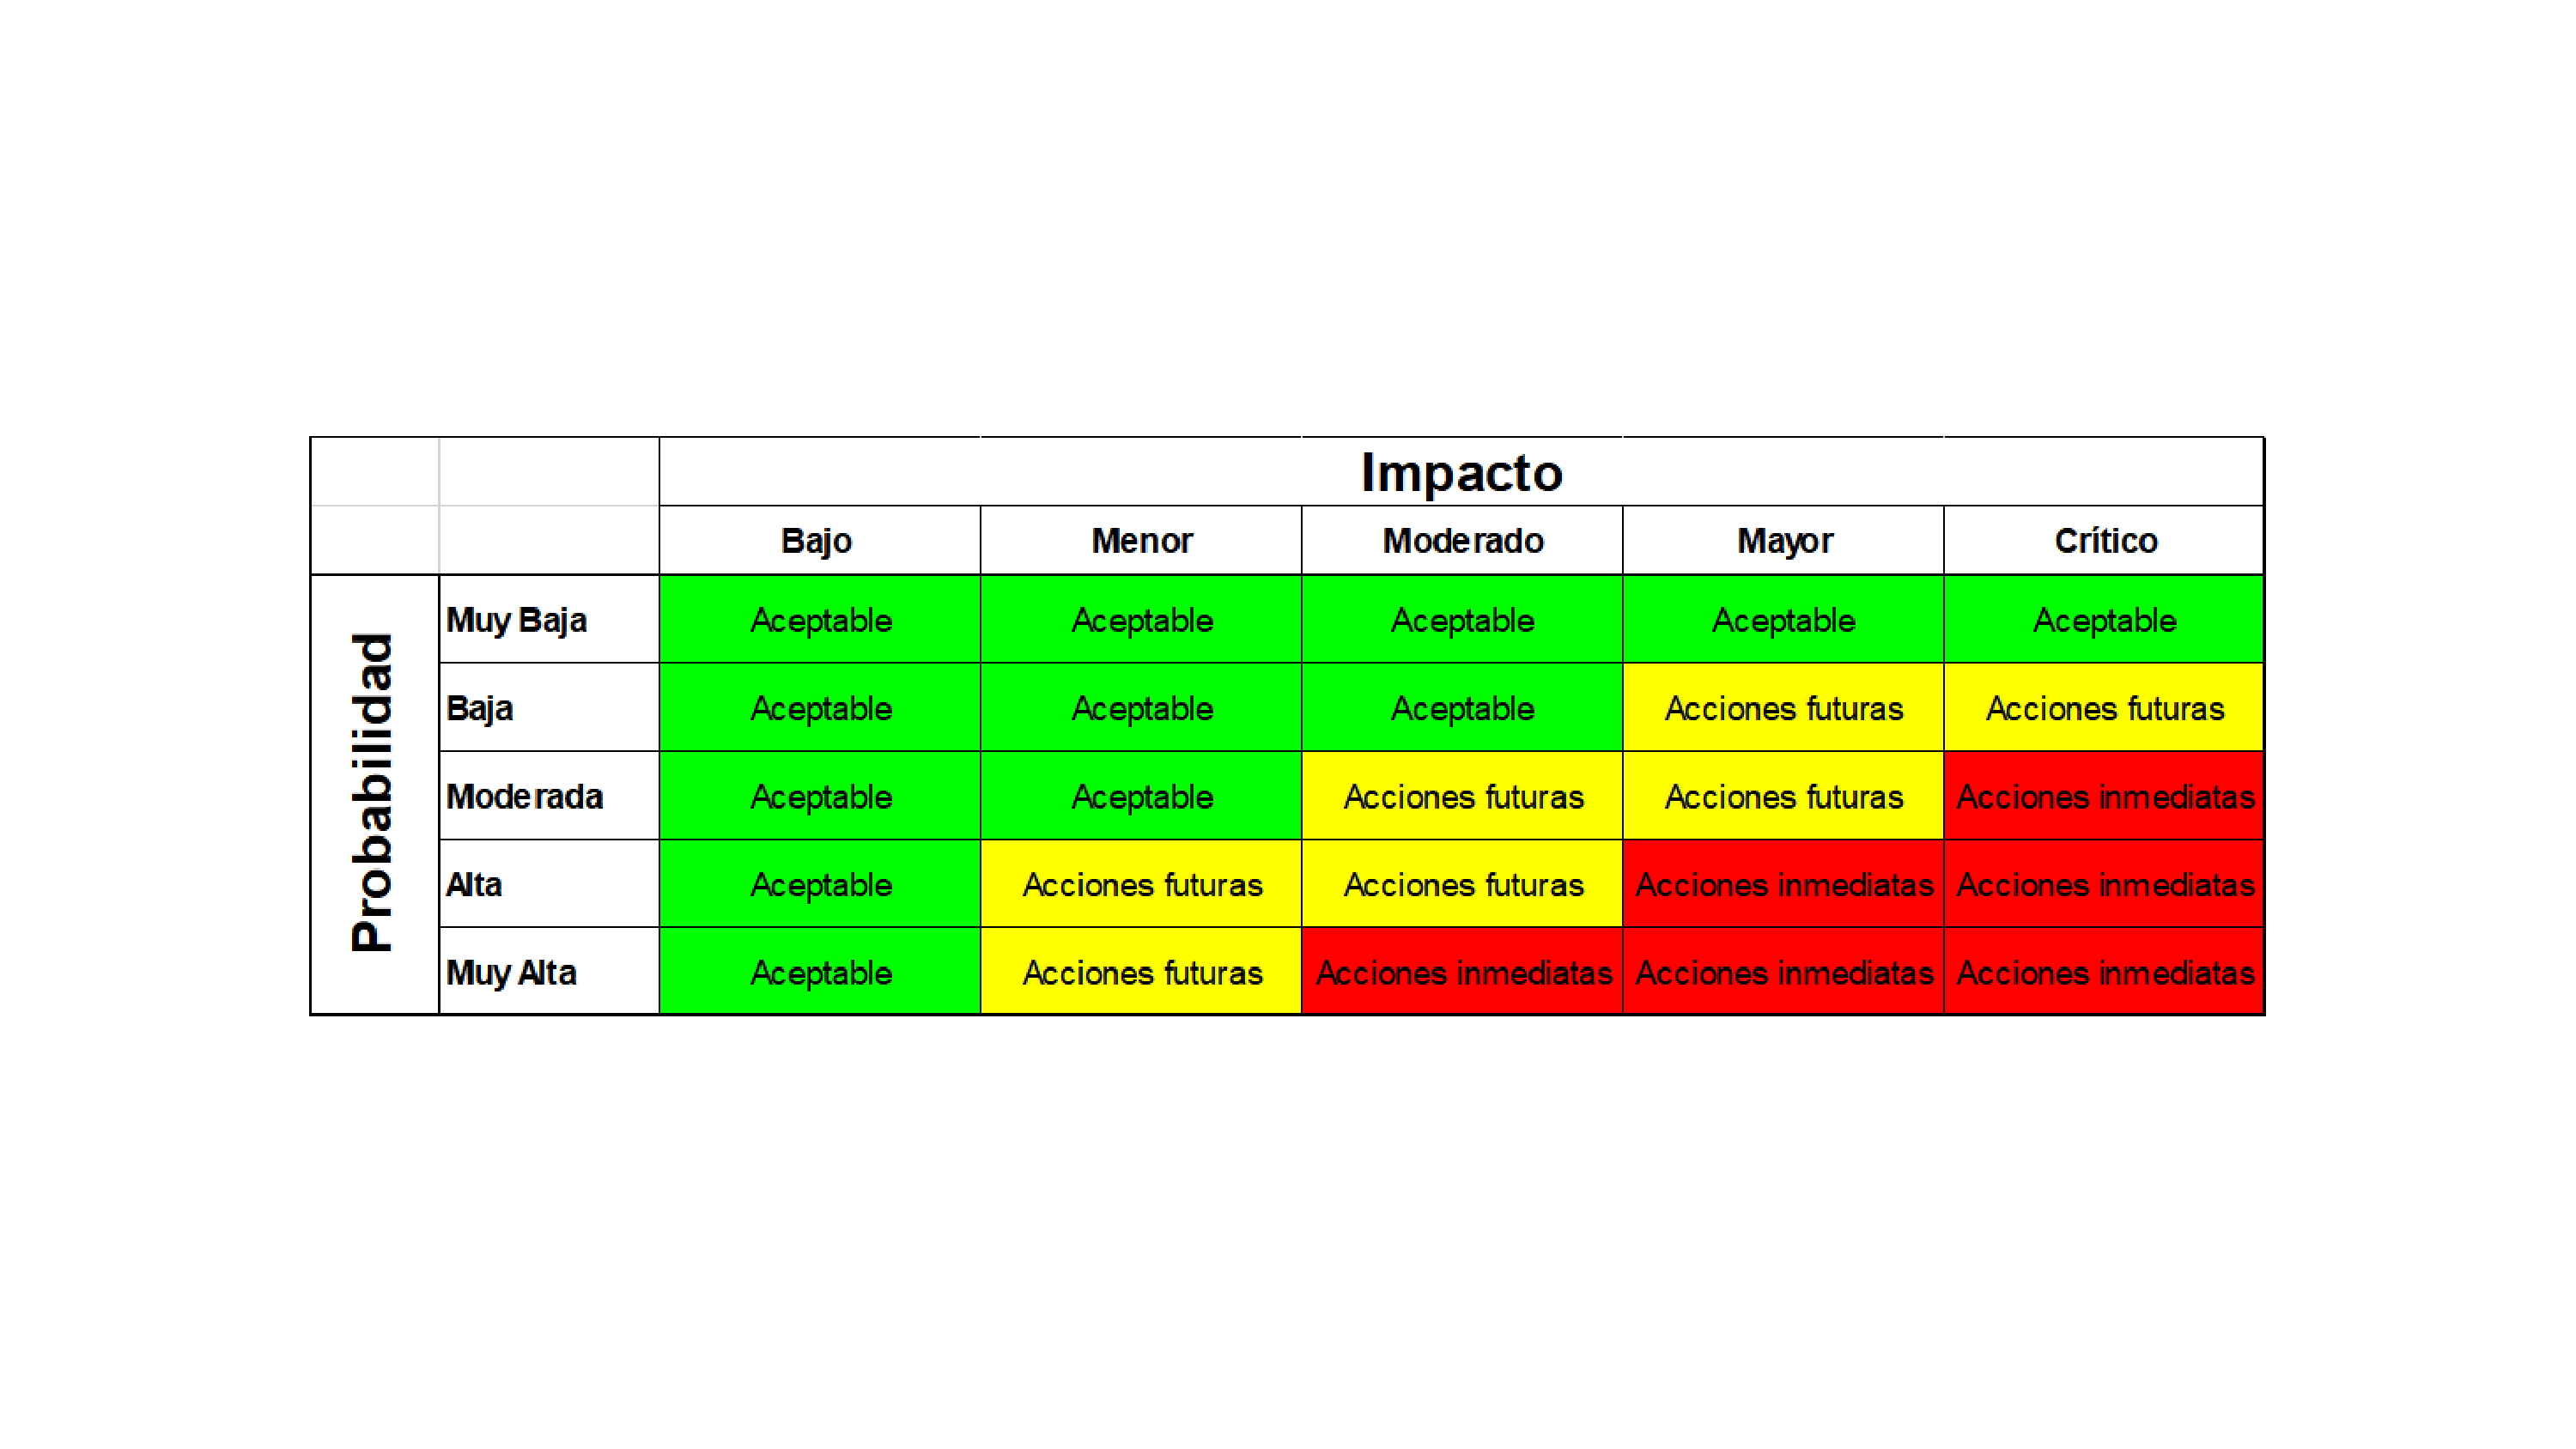
\includegraphics[scale=0.17]{30/img/TablaDeRiesgo.pdf}
        \caption{Diagrama para la identificación de riesgos y acciones}
        % \label{fig:my_label}
    \end{figure}
    % 
    % 
    \subsubsection{Riesgos internos}
    
    El concepto de riesgo se relaciona con la posibilidad de que un evento ocurra, lo que indica la cercanía de un posible daño. En términos más simples, se refiere a la probabilidad de que algo suceda. Los riesgos identificados se muestran en la siguiente tabla.
    
    Por otro lado, el riesgo operativo interno se define como la probabilidad de que la empresa sufra pérdidas debido a fallos o deficiencias en sus propios procesos o funciones naturales de operación. En resumen, se trata de los riesgos que surgen dentro de la empresa como resultado de su propio funcionamiento.
    % 
    % 
    \begin{figure}[H]
        \centering
        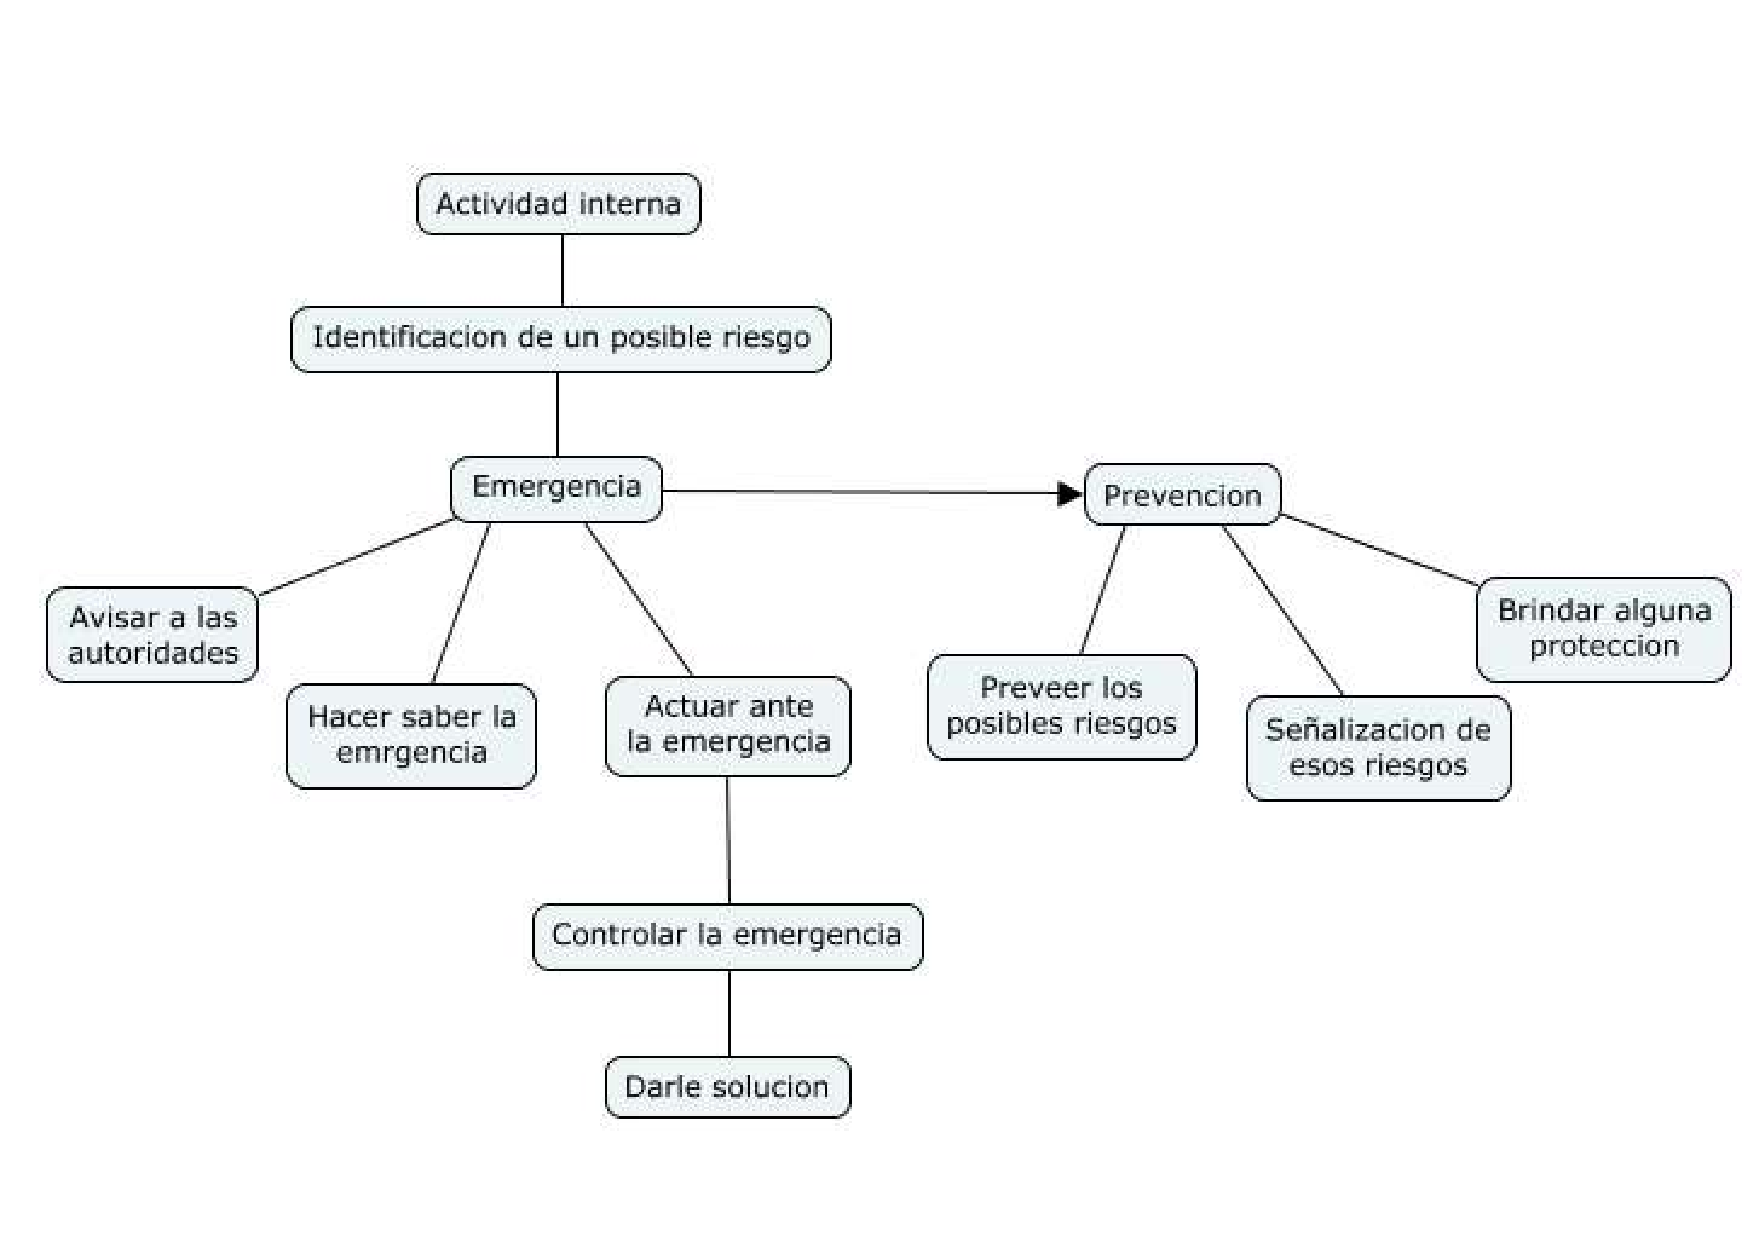
\includegraphics[scale=0.185]{30/img/RiesgosInternos.pdf}
        \caption{Diagrama para la identificación de riesgos y acciones}
        % \label{fig:my_label}
    \end{figure}
    % 
    % 
    % 
    % \begin{table}[h]
    %     \centering
    %     \caption{Descripción de los riesgos al realizar las actividades más comunes y de riesgo dentro de la empresa}
    %     \begin{tabular}{|c|c|c|c|p{7em}|c|}
    %          \hline
    %          Causa& Descripción del riesgo& Probabilidad& Impacto& Acciones Preventivas& Responsable \\
    %          \hline
    %          Gestión& Herida lacerada& 0.01 Bajo& Muy bajo& No utilizar navaja solo cúter&  \\
    %          \hline
    %          Gestión& Golpe con martillo& 0.01 Bajo& Muy bajo& Capacitación&  \\
    %          \hline
    %          Gestión& Levantar super sacos& 0.17 Medio& bajo& Utilizar faja y recibir ayuda&  \\
    %          \hline
    %          Gestión& Carga de camionetas& 0.01 Bajo& Muy bajo& Utilizar faja y guantes&  \\
    %          \hline
    %          Cliente& Descarga de camioneta& 0.17 medio& bajo& Utilizar faja y guantes&  \\
    %          \hline
    %          Gestión& Corto circuito& 0.17 medio& bajo& Revisar las conexiones de la fuente de energía cada mes&  \\
    %          \hline
    %          Cliente& Fumador& 0.01 Bajo& Muy bajo& Señalamientos y llamada de atención&  \\
    %          \hline
    %     \end{tabular}
    %     \label{tab:Riesgos}
    % \end{table}
    % 
    \begin{figure}[H]
        \centering
        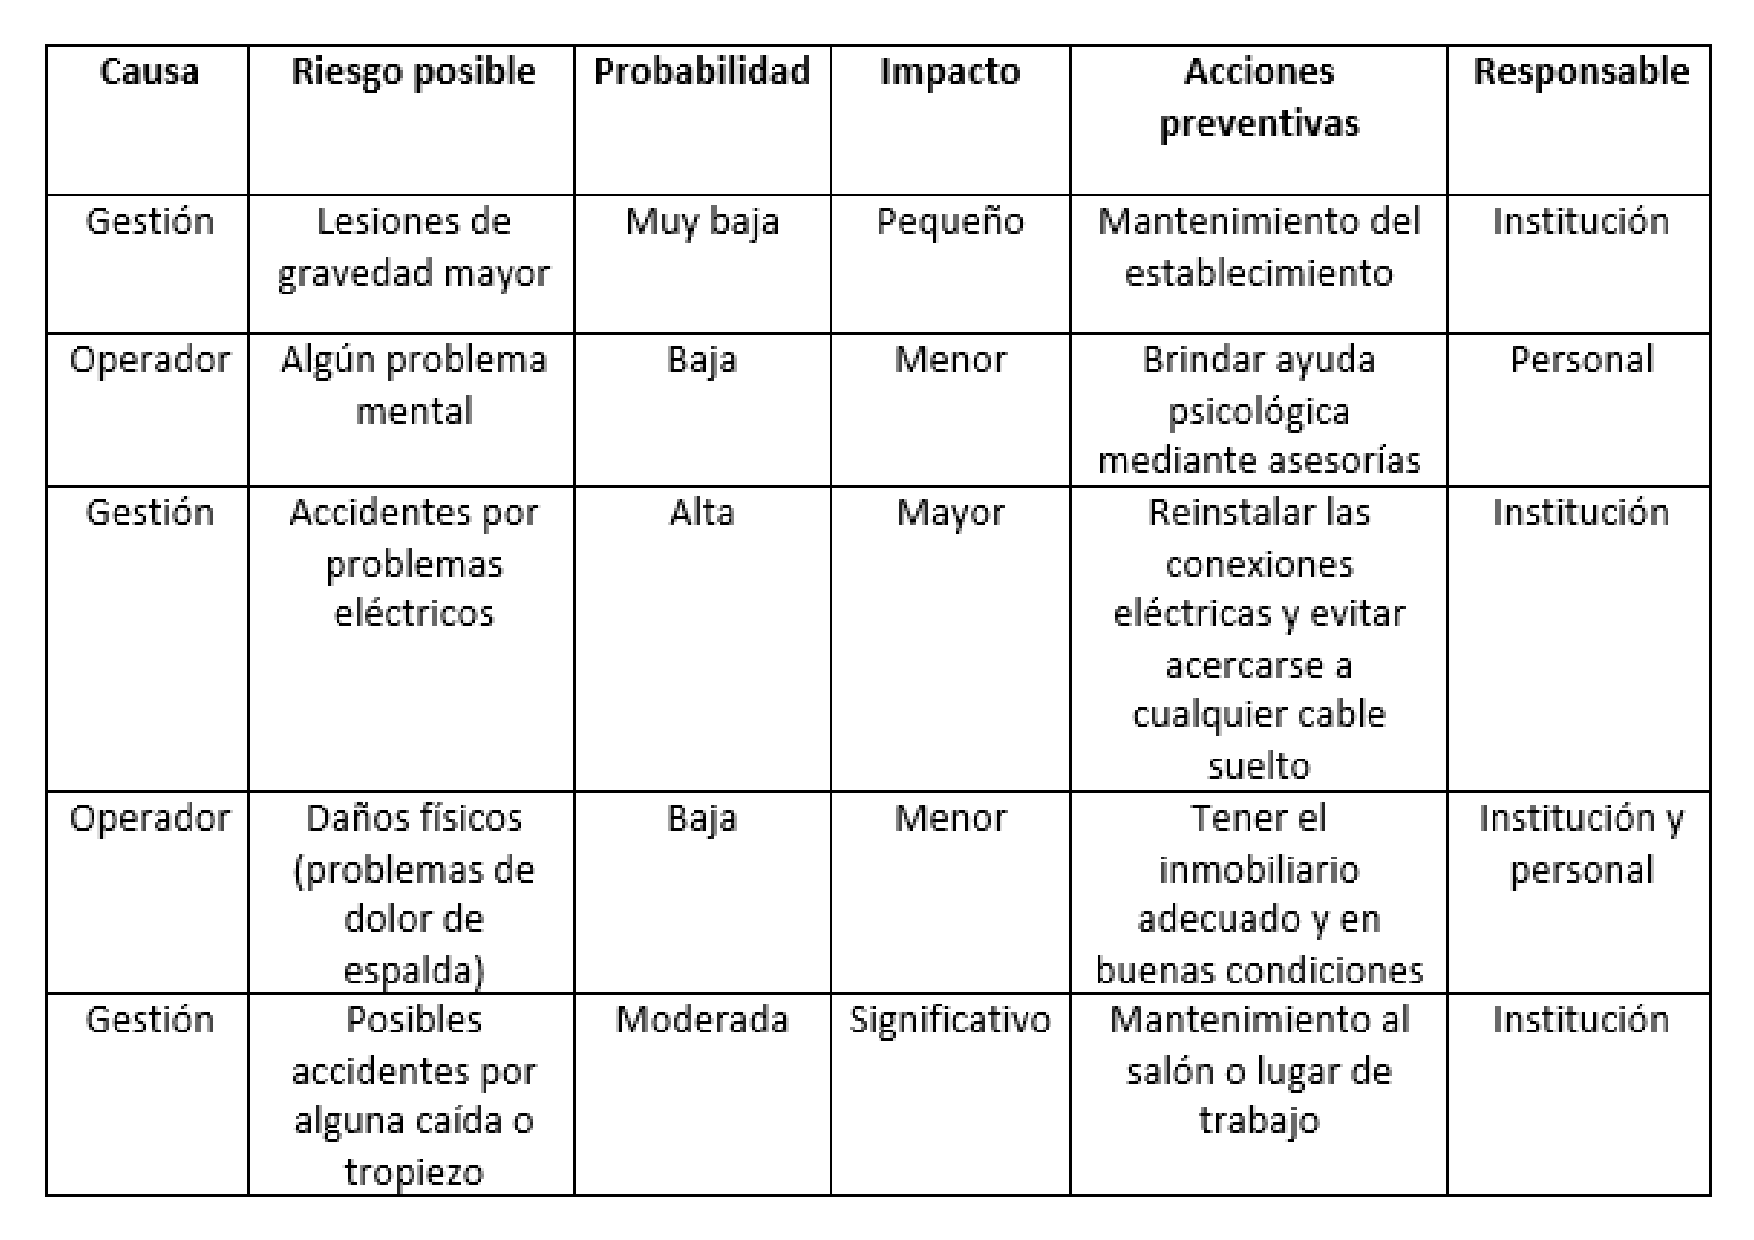
\includegraphics[scale=0.25]{30/img/PosiblesRiesgosInt.pdf}
        \caption{Posibles riesgos al realizar las actividades más comunes y de riesgo dentro del aula}
        % \label{fig:my_label}
    \end{figure}
    % 
    % 
    \subsubsection{Riesgos externos}
    Por otro lado, el riesgo operativo externo se refiere a la posibilidad de que la empresa sufra interrupciones o pérdidas debido a factores externos que escapan a su control y que afectan su funcionamiento. Específicamente, estos riesgos surgen del entorno externo de la empresa, como cambios en las políticas gubernamentales, desastres naturales y situaciones de inseguridad en el área circundante. Estos riesgos son resultado de influencias externas y no de deficiencias internas en los procesos o funciones de la empresa.
    
    \begin{figure}[H]
        \centering
        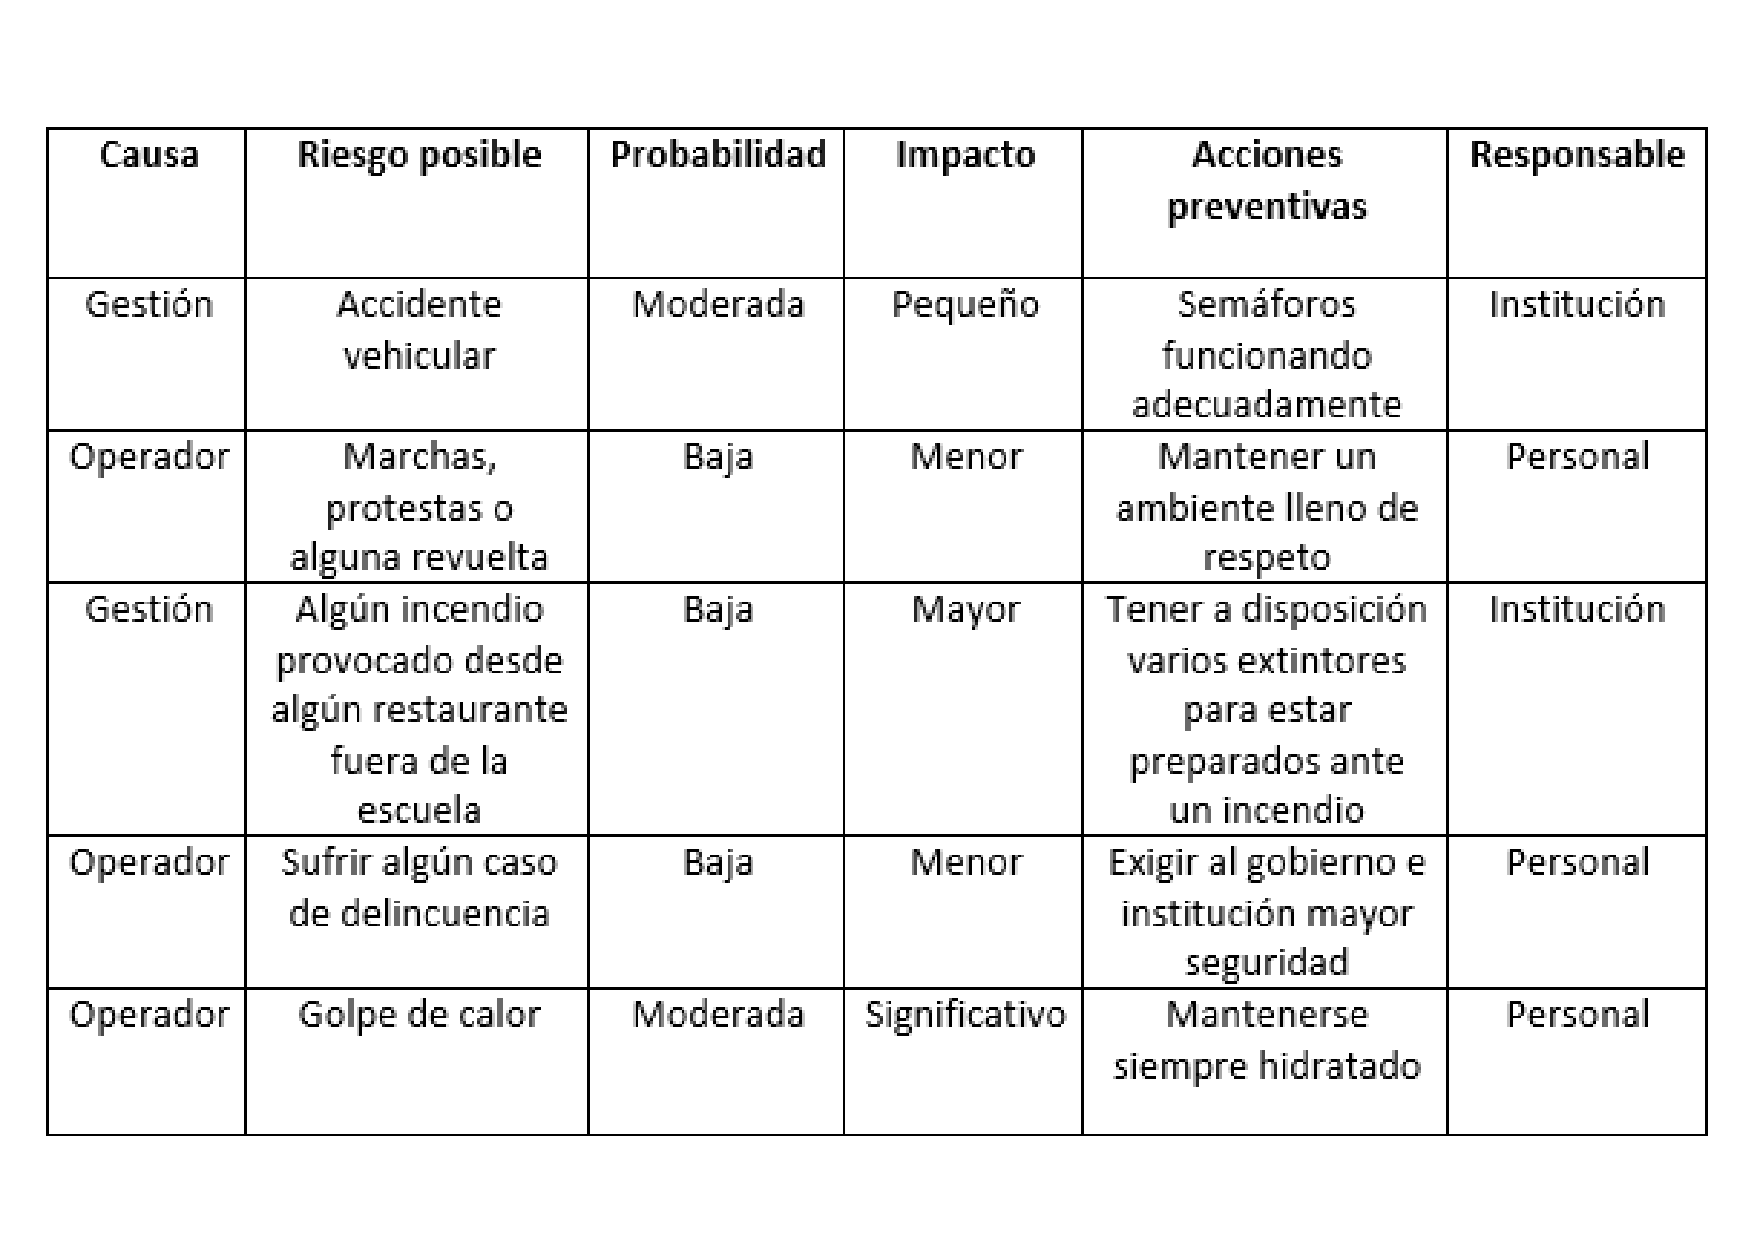
\includegraphics[scale=0.25]{30/img/PosiblesRiesgosExt.pdf}
        \caption{Diagrama para la identificación de riesgos externos}
        % \label{fig:my_label}
    \end{figure}
    % 
    % \begin{table}[H]
    %     \centering
    %     \caption{Descripción de los riesgos externos}
    %     \begin{tabular}{|c|c|c|p{10em}|}
    %          \hline
    %          Descripción del riesgo& Probabilidad& Impacto& Acciones preventivas\\
    %          \hline
    %          Desmayo del cliente& 0.01 bajo& Muy bajo& Colocar al cliente en una posición apropiada para la llegada de los paramedicos\\
    %          \hline
    %          Incendio de algún vecino& 0.01 bajo& Alto& Mantener los detectores de humo en lugares estratégicos y con pilas\\
    %          \hline
    %          Incendio de camioneta& 0.17 moderado& Alto& Mantener en mantenimiento los sensores de temperatura y con un extintor \\
    %          \hline
    %          Incendio por pirotecnia& 0.17& Alto& Vigilar en los días festivos y mojar el material\\
    %          \hline
    %          Choque en la avenida& 0.17& Medio& Delimitar y poner conos de señalamiento\\
    %          \hline
    %     \end{tabular}
    %     \label{tab:RiesgosExternos}
    % \end{table}
    % 
    % 
    % 
    \subsubsection{Programa de actividades de prevención y auxilio}
    
    Declaramos las diferentes acciones de lo que se piensa hacer cuando ocurra un riesgo interno u externo. 
    Las actividades de preparación y disposición que se hace anticipadamente en el ITP para evitar riesgos.
    % 
    % 
    \subsubsection{Plan de acción}
    
    El plan estratégico de acciones del ITQ es un conjunto organizado de directrices que capacitan a la institución para abordar una amplia gama de situaciones, desde resolver problemas internos hasta manejar eficazmente riesgos externos. Este plan detalla medidas específicas que deben tomarse en caso de que surjan riesgos, tanto dentro como fuera de la institución. Incluye procedimientos claros de respuesta, asignación de responsabilidades, recursos necesarios y un cronograma para su ejecución. Además, se desarrolla de manera proactiva, identificando anticipadamente posibles riesgos y adoptando medidas preventivas para reducir su impacto. Este enfoque garantiza que el ITQ esté preparado para enfrentar cualquier desafío que se presente, protegiendo así los intereses y la seguridad de la comunidad universitaria.
    % 
    % 
    % \begin{table}[H]
    %     \centering
    %     \caption{Descripción de las acciones anticipadas y correctivas ante un riesgo interno}
    %     \begin{tabular}{|p{5em}|p{10em}|p{11em}|p{10em}|}
    %         \hline
    %          RIESGO INTERNO& Acción Anticipada& Acción Correctiva& Indicador\\
    %          \hline
    %          Herida lacerada& Reemplazar las navajas y cuchillos por cutter con resorte. Utilizar en lo menos posible objetos punzo cortantes& Utilizar el material de los primeros auxilios y lavar la herida con agua oxigenada y vendar& Constancias de capacitación así como el registro de la disminución en el uso de curitas\\
    %          \hline
    %          Golpeo con martillo& Capacitación y descansos de 5 minutos cuando se este trabajando constantemente con el martillo& Aplicar pomada para golpes del botiquín de primeros auxilios& Menos reportes de golpes\\
    %          \hline
    %          Levantar super sacos& Capacitar con el uso adecuado de la faja y solicitar ayuda al momento de levantar materiales mayores a 30 kg& Tomar un descanso y tomar agua &Disminución del cansancio al final del día\\
    %          \hline
    %          Carga y descarga de camionetas& Capacitar con el uso adecuado de la faja y solicitar ayuda al momento de levantar materiales mayores a 30 kg& Utilizar más personal para evitar riesgos & Menor tiempo de carga y descarga en la camioneta\\
    %          \hline
    %          Chispa por cigarro& Señalamientos de no fumar a la entrada& Pedir de manera amable que apaguen el cigarro& Observar en el área de trabajo decremento de las colillas de cigarro\\
    %          \hline
    %          Corto circuito& Mantenimiento preventivo en los fusibles en el centro de carga& Bajar los interruptores del centro de carga& Obtención de un reporte técnico por lo menos una vez al año\\
    %          \hline
    %     \end{tabular}
    %     \label{tab:my_label}
    % \end{table}
    % 
    % 
    \begin{figure}[H]
        \centering
        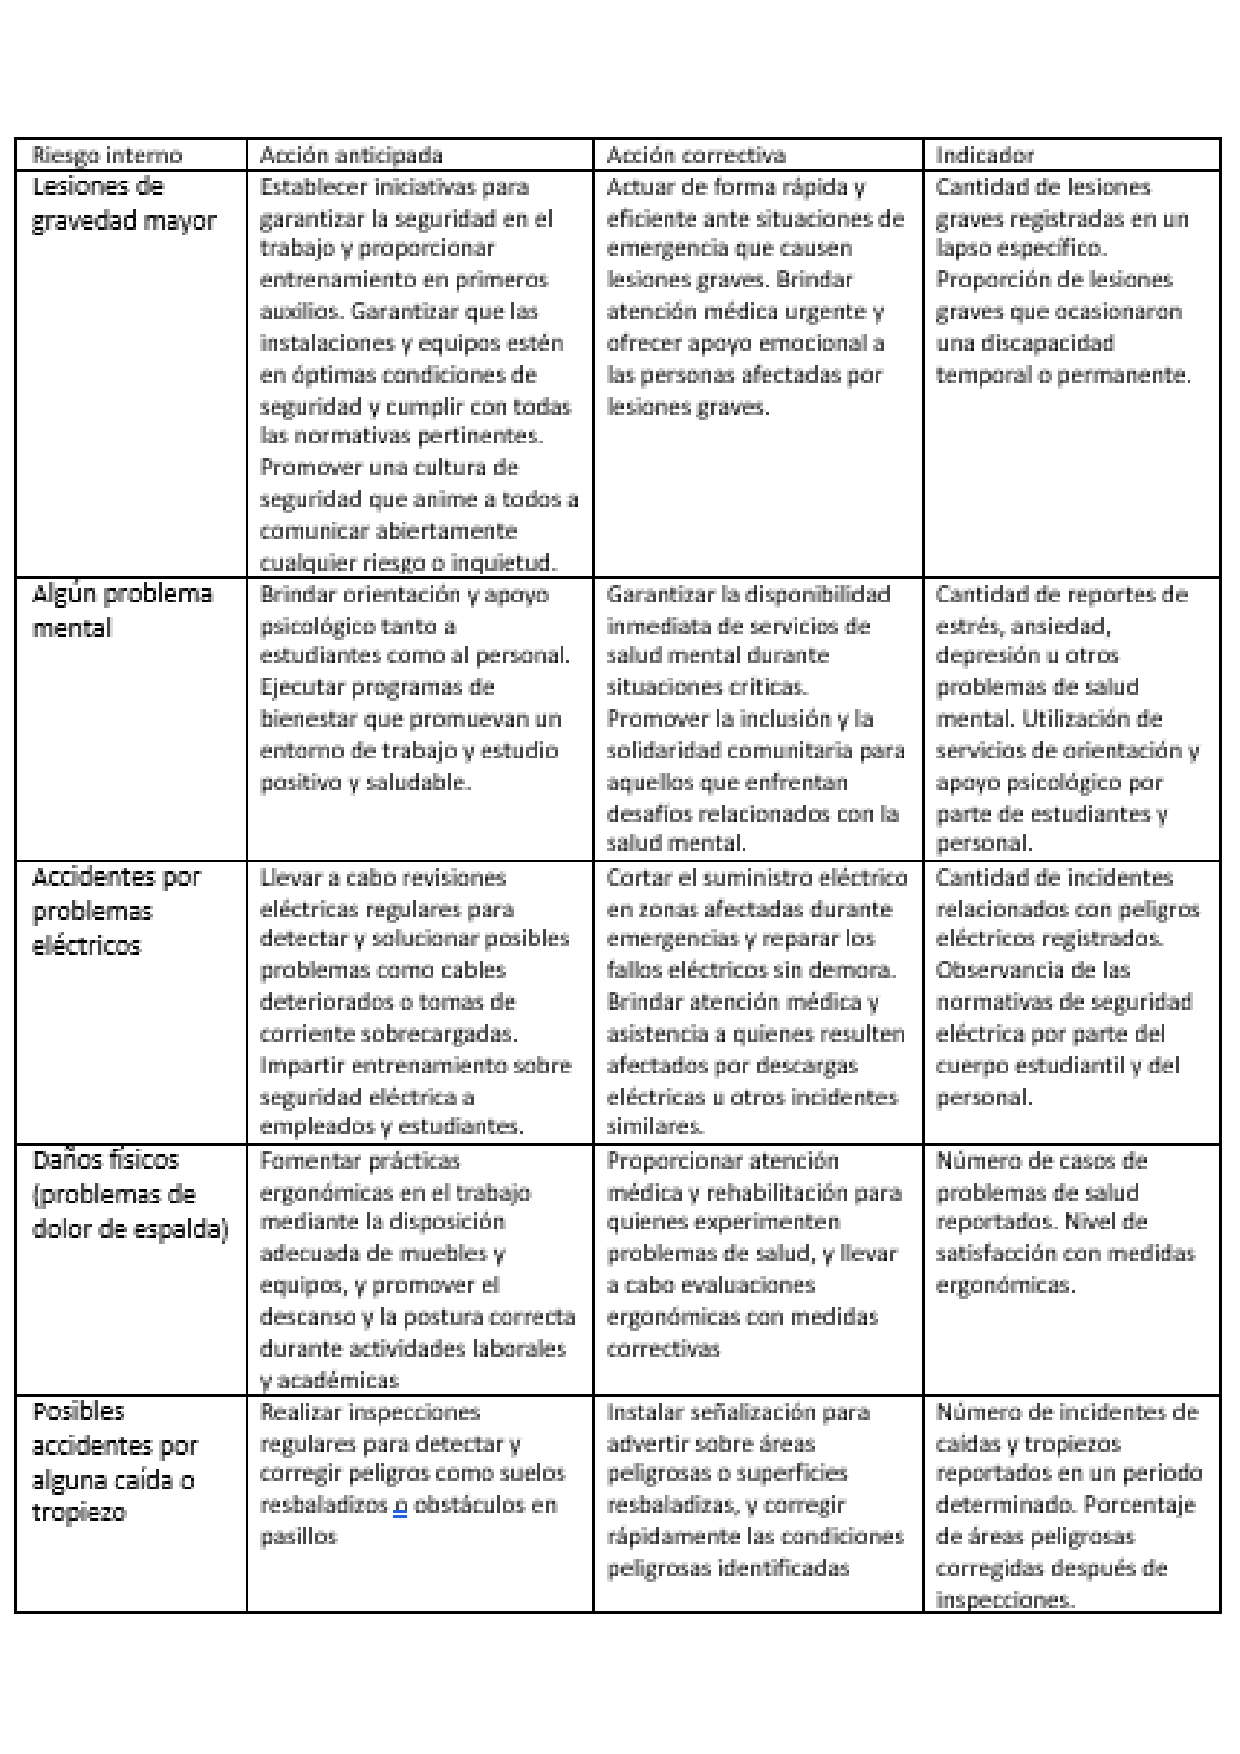
\includegraphics[scale=0.25]{30/img/TablotaDeRiesgosint.pdf}
        \caption{Riesgo interno y sus acciones anticipadas y correctivas}
        % \label{fig:my_label}
    \end{figure}
    % 
    % 
    % \begin{table}[H]
    %     \centering
    %     \caption{Descripción de las acciones anticipadas y correctivas ante un riesgo externo e interno}
    %     \begin{tabular}{|p{5em}|p{10em}|p{11em}|p{10em}|}
    %          \hline
    %          RIESGO EXTERNO& Acción Anticipada& Acción Correctiva& Indicador\\
    %          \hline
    %          Desmayo del cliente& Tomar cursos de primeros auxilios por lo menos una vez al año a todo el personal& Contar con los conocimientos básicos de primeros auxilios& Realizar un simulacro que nos permita evaluar las acciones en el manejo del riesgo por desmayo\\
    %          \hline
    %          Incendio de algún vecino& Mantener los detectores de humo en lugares estratégicos y cambiar las pilas cada 2 meses& Llamar al 911 para informar del incendio y del posible riesgo en el negocio&  Llevar un registro de los cambios de las pilas en los detectores de humo\\
    %          \hline
    %          Incendio de camioneta& Mantener en mantenimiento los sensores de temperatura y con un extintor& Accionar el extintor conforme a lo establecido por el departamento de bomberos y llamar al 911& Revisar el tablero de la camioneta que no indique falta de agua o alta temperatura \\
    %          \hline
    %          Incendio por pirotecnia& Vigilar en los días festivos y mojar el material& Llamar a emergencias y tratar de sofocar el fuego& Hacer un llamado a los vecinos a ser cuidadosos\\
    %          \hline
    %          Choque en la avenida& Delimitar y poner conos de señalamiento& Llamar a emergencias y si es que hay daños a personas, aplicar primeros auxilios en caso de ser necesario& Llevar un registro de las horas pico para evitar hacer maniobras\\
    %          \hline
    %     \end{tabular}
    %     \label{tab:Acciones}
    % \end{table}
    % 
    % 
    \begin{figure}[H]
        \centering
        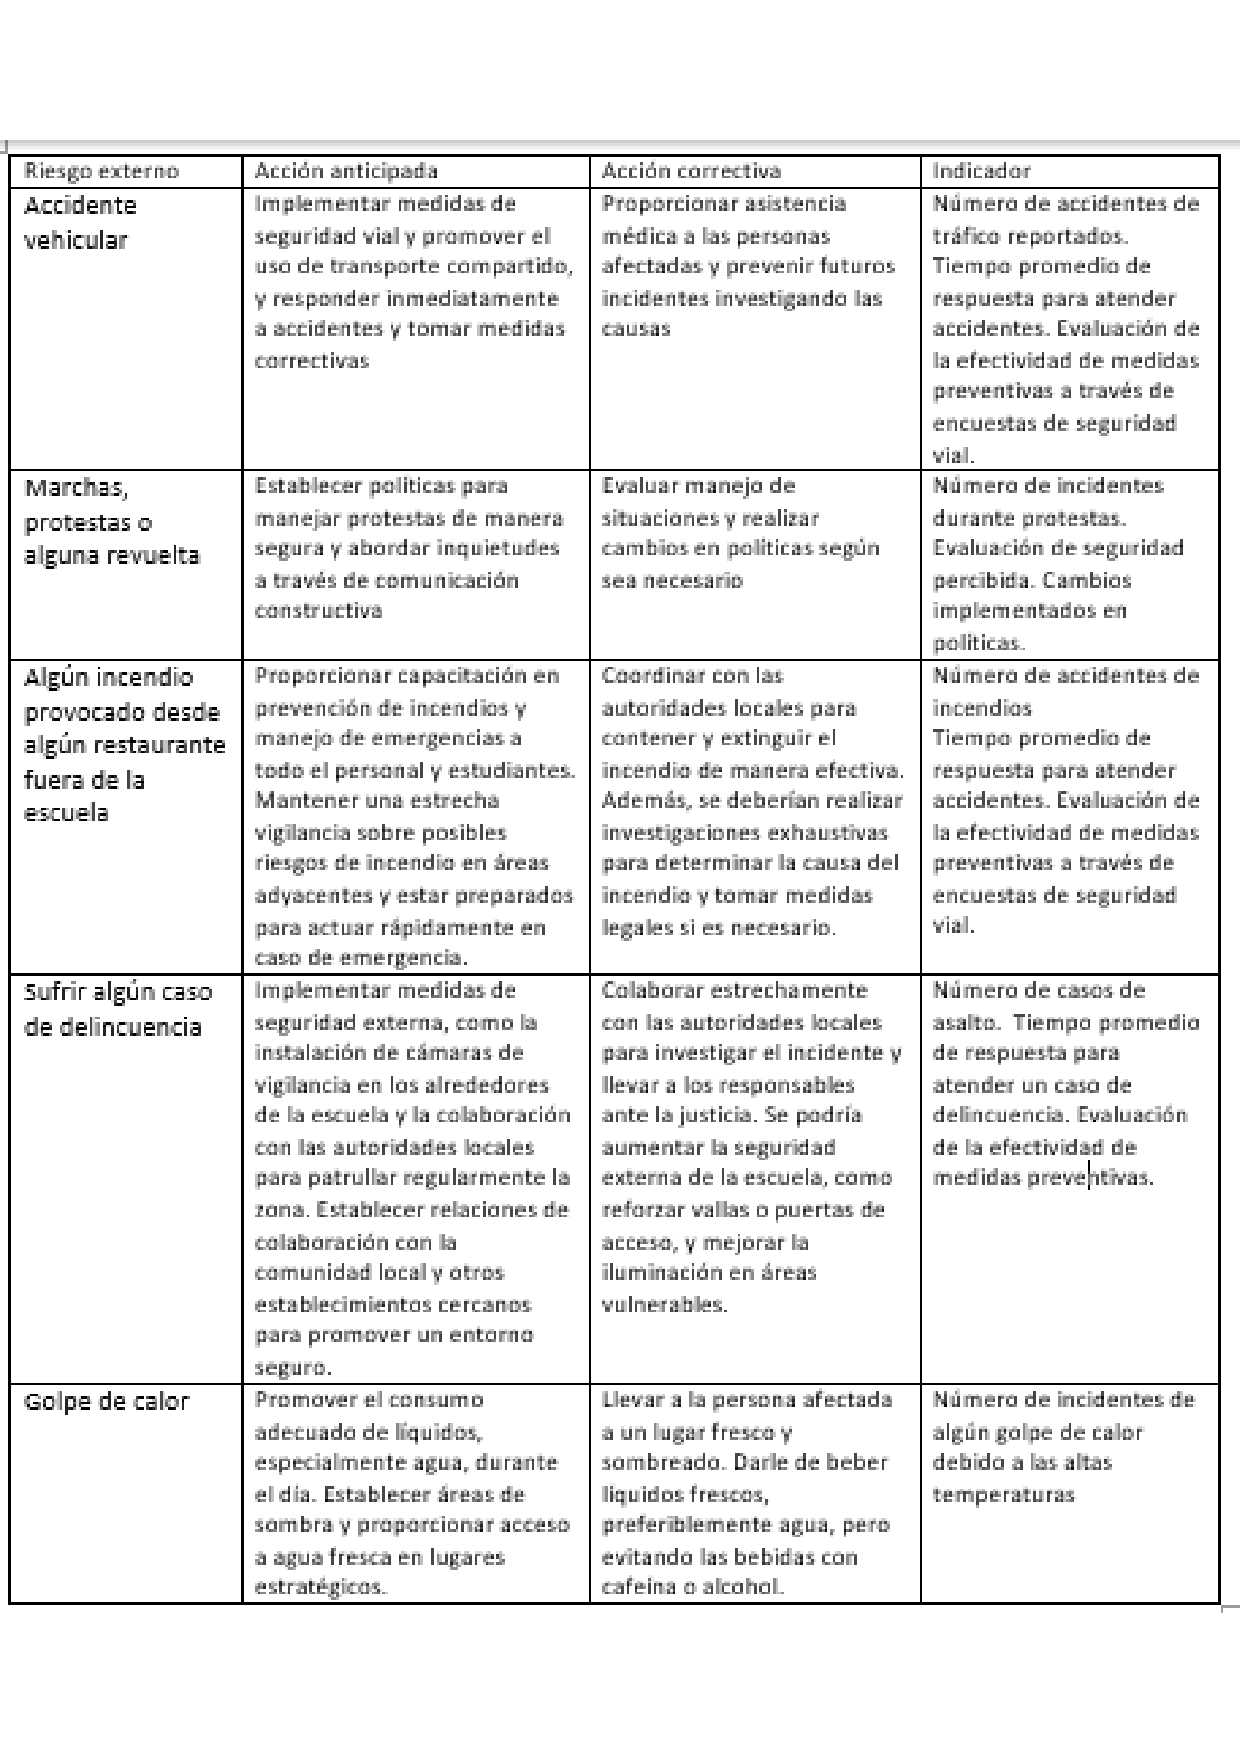
\includegraphics[scale=0.25]{30/img/TablotaDeRiesgoext.pdf}
        \caption{Riesgo externo y sus acciones anticipadas y correctivas}
        % \label{fig:my_label}
    \end{figure}
    % 
    % 
    % Cada estrategia metodológica se establece acorde a cada objetivo, y por tanto deberá ser desglosada precisada y ordenada claramente. En consecuencia cada objetivo que se presentó en forma de verbo en infinitivo deberá determinar una estrategia en forma de adverbio. Ej. Desarrollar…Desarrollo. Son las actividades ordenadas que tienen como finalidad la prueba de la hipótesis. 
    
    % \begin{itemize}
    %     \item Se debe establecer que se habrá de hacer, como, conque, y donde para obtener la información que permita probar la hipótesis.  
    %     \item Se debe desglosar de acuerdo a los objetivos específicos. 
    %     \item Se debe establecer una estrategia metodológica por cada objetivo específico. De manera simplista se podría decir que se cambia el verbo en infinitivo por su respectivo adverbio.
    %     \item En cada objetivo se debe describir que método, que materiales y que equipo se usará para conseguirlo.
    %     \item Se deben tener referencias Figura \ref{fig:lcd-16x2}.
    % \end{itemize}
    % 
    % 
    % \begin{figure}[H]
    %     \centering
    %     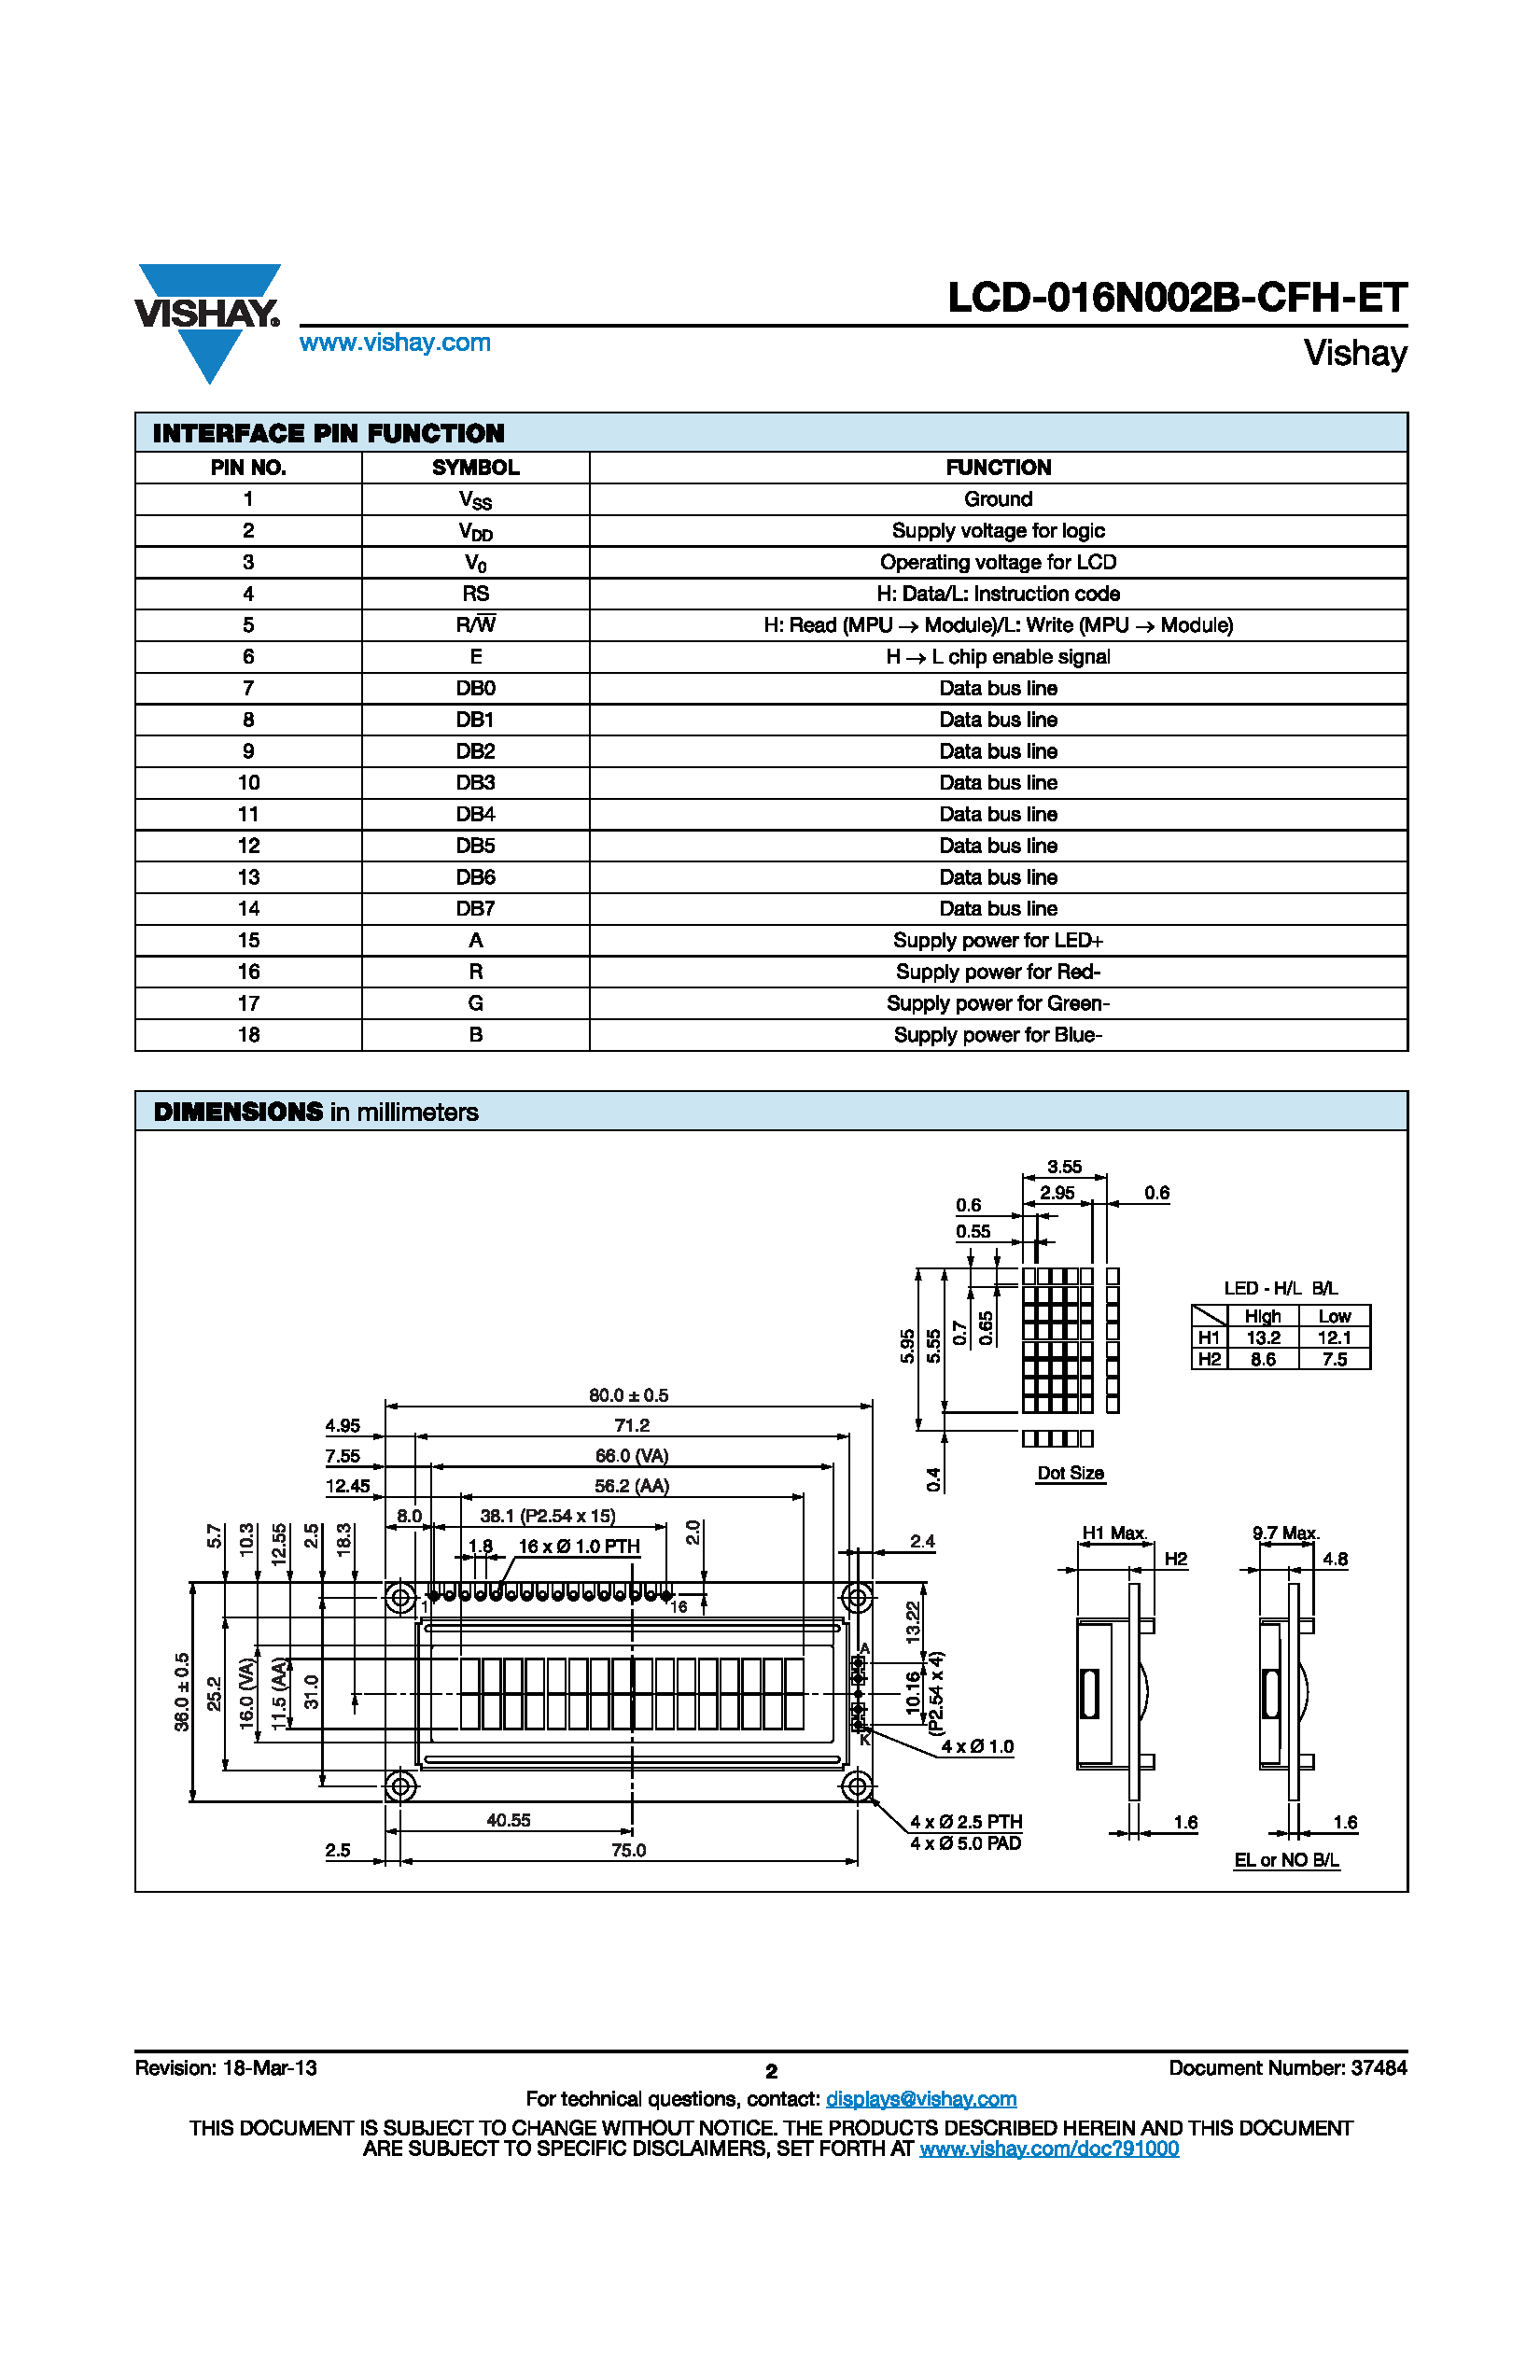
\includegraphics[trim = {30mm 65mm 90mm 250mm},clip,scale=0.5]{6/Img/lcd-16x2.pdf}
    %     \caption{Esquema LCD de 16x2}
    %     \label{fig:lcd-16x2}
    % \end{figure}
    % 
    % 
    % \begin{figure}[H]
    %     \centering
    %     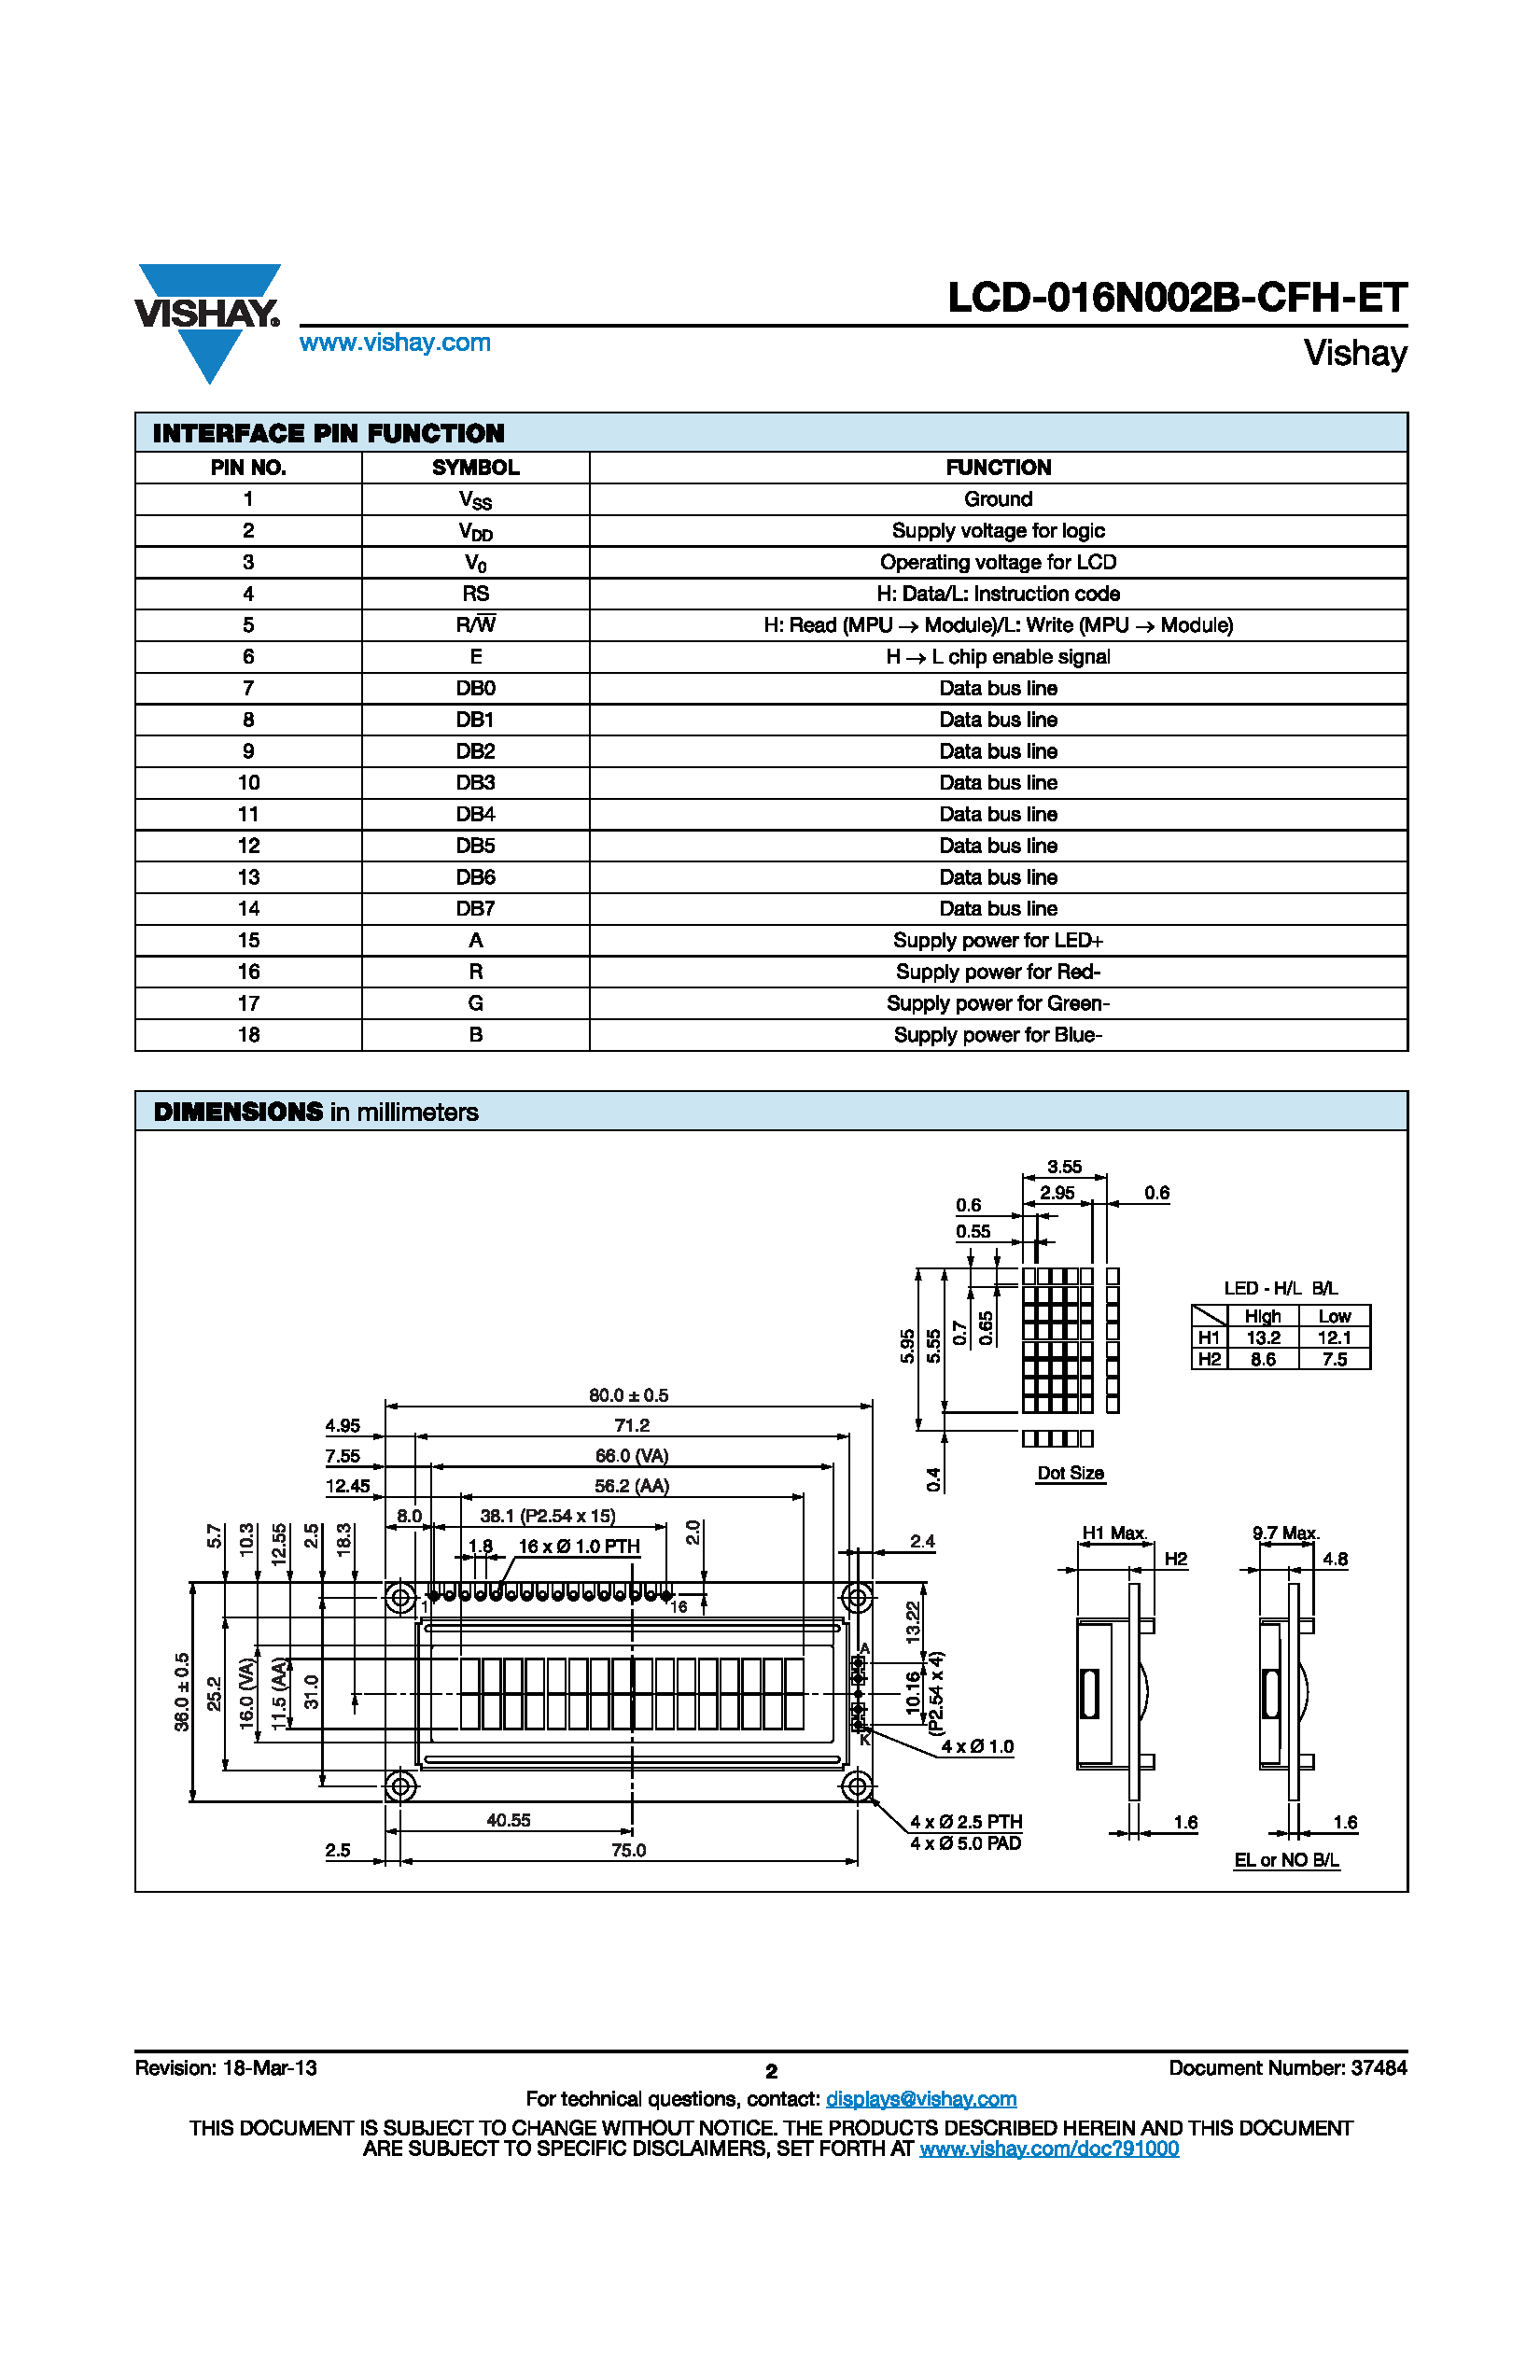
\includegraphics[trim = {30mm 250mm 90mm 20mm},clip,scale=0.5]{6/Img/lcd-16x2.pdf}
    %     \caption{Esquema LCD de 16x2}
    %     \label{fig:lcd}
    % \end{figure}
    % 
    % 
    % \subsection{Prepara tu documento}
    
    % Antes de que comiences a utilizar esta plantilla, es recomendable que prepare la información que contendrá en un archivo aparte. 
    % Ten preparadas tus gráficas, así como también las tablas aparte, para que sea más fácil integrarlo. 
    % Se recomienda fuertemente el uso de \textbf{formato Enhanced Metafile (.emf) para imágenes y gráficas} de resolución óptima. 
    % Finalmente, completa y organiza el contenido antes de darle el formato de esta plantilla. 
    % 
    % 
    \subsubsection{Identificación de capacidades}
    
    \begin{table}[H]
        \centering
        \caption{Recursos en materia de seguridad}
        \begin{tabular}{c c c}
        \hline
        \multicolumn{3}{c}{Inventario de recursos en materia de seguridad}\\
        \hline
             No.& Recurso & Cantidad  \\
        \hline
             1& Extintor & 3  \\
        \hline
             2& Botiquín & 1  \\
        \hline
             3& Detector de humo & 1 \\
        \hline
             4& Lampara de emergencia & 1 \\
        \hline     
        \end{tabular}
        \label{tab:inventario}
    \end{table}
    % 
    % 
    \subsubsection{Plano de localización de recursos}
    
    % 
    % 
    
    % 
    % 
    \subsubsection{ Identificación de apoyos externos}
    \begin{figure}[H]
        \centering
        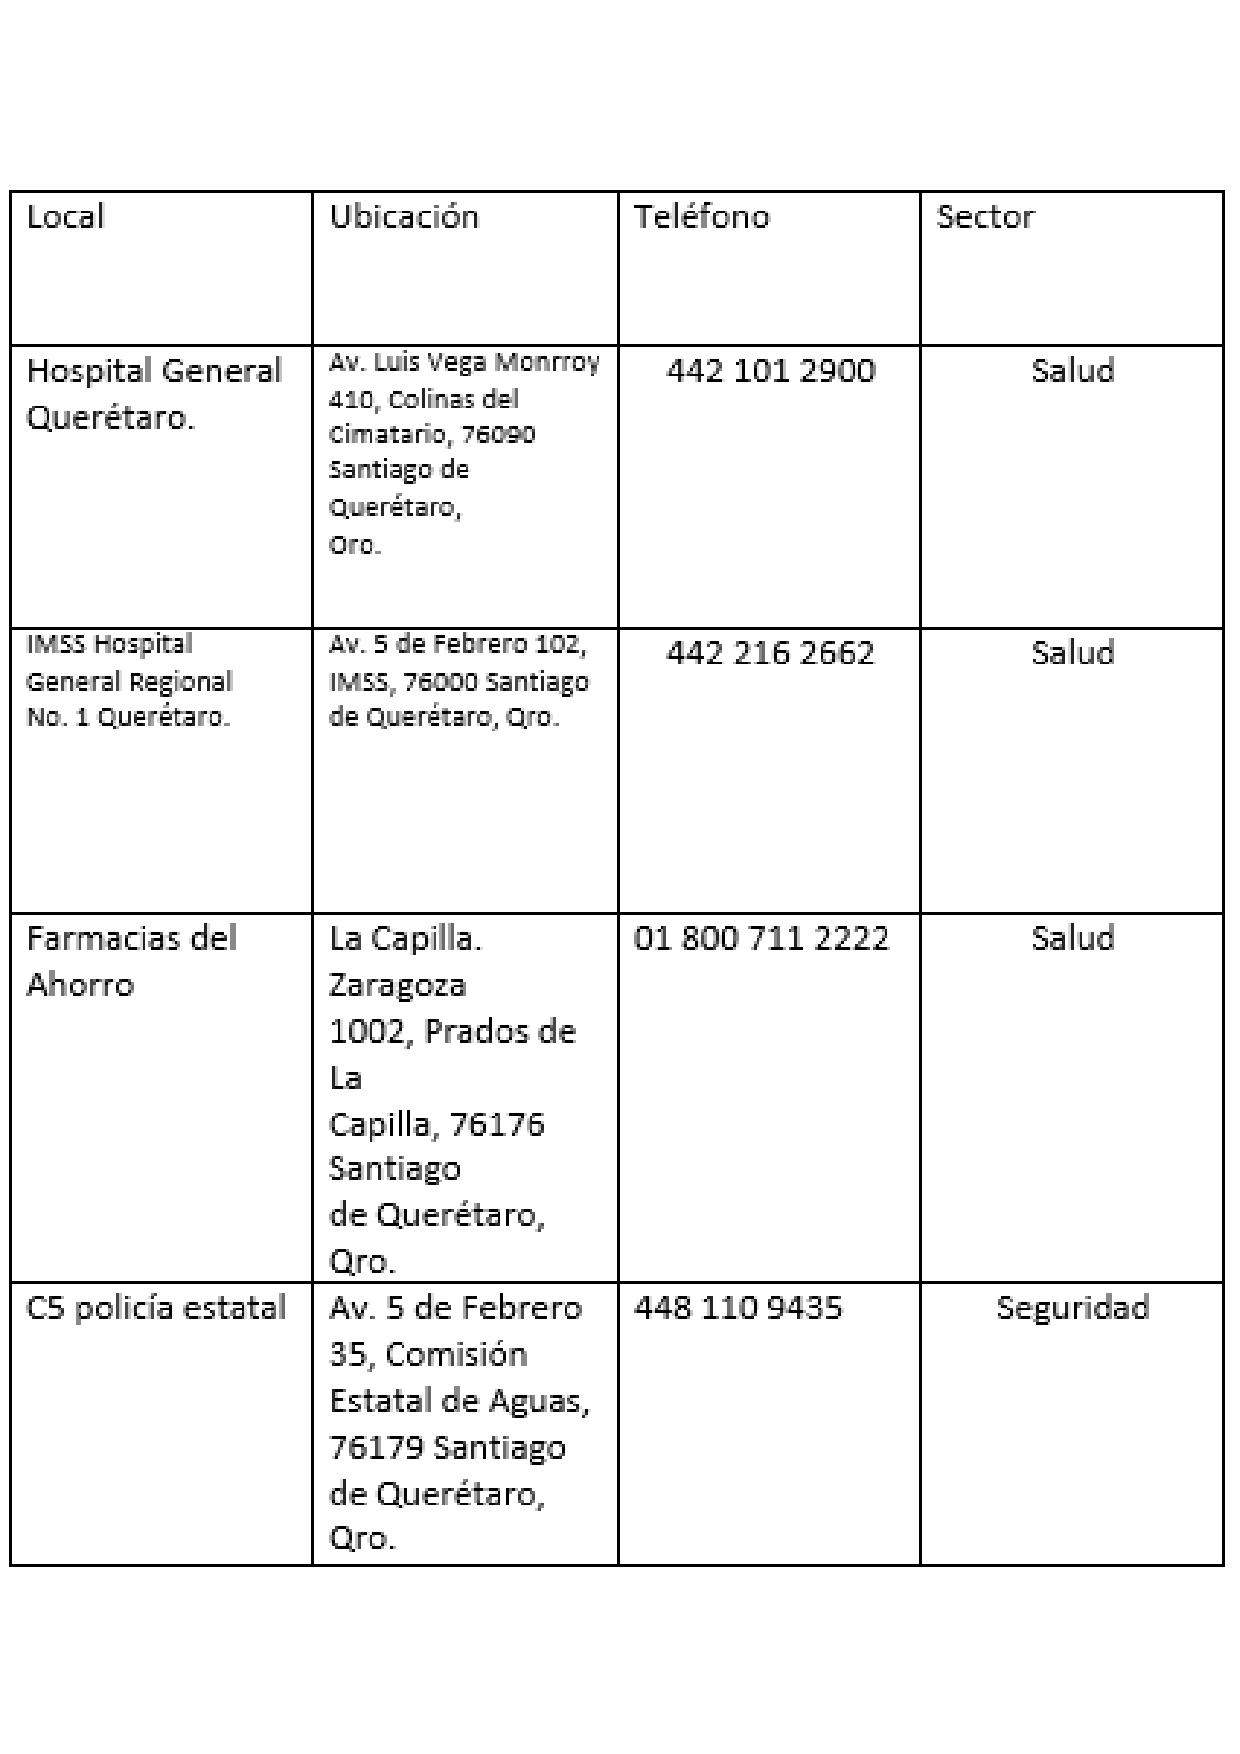
\includegraphics[scale=0.25]{30/img/apoyosExternos.pdf}
        \caption{Apoyos externos para una situación de emergencia}
        % \label{fig:my_label}
    \end{figure}
    
    % 
    % 
    \subsubsection{Identificación de puntos de reunión}
    \begin{figure}[H]
        \centering
        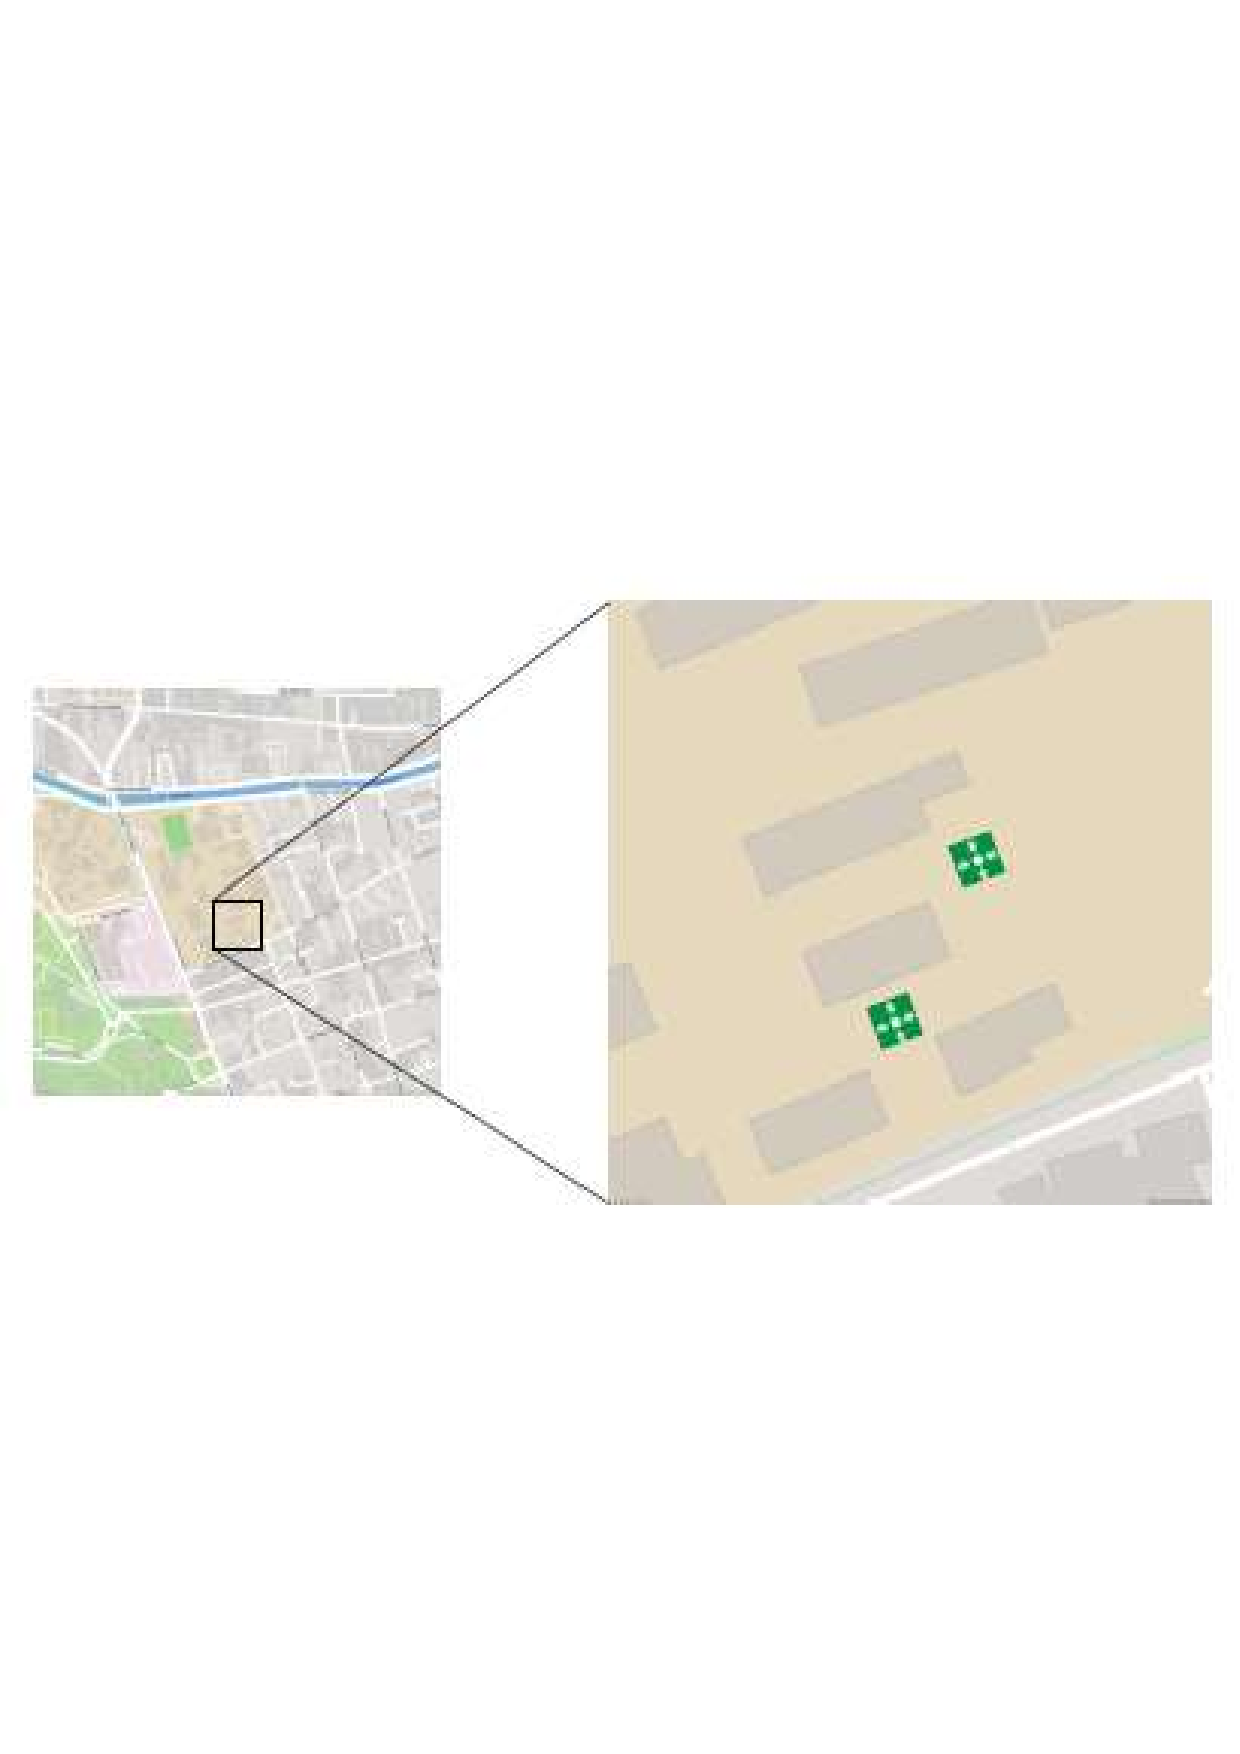
\includegraphics[scale=0.25]{30/img/puntoDeReunion.pdf}
        \caption{Identificación de los puntos de reunión dentro de la escuela}
        % \label{fig:my_label}
    \end{figure}
    
    % 
    % 
    \subsubsection{Brigada de evacuación}
    
    
    % 
    % 
    \subsubsection{Directorio de telefónicos de emergencia}
    
    Listado telefónico de instituciones de atención de emergencias y otras instituciones que intervengan para el seguimiento y control de las mismas.
    \begin{figure}[H]
        \centering
        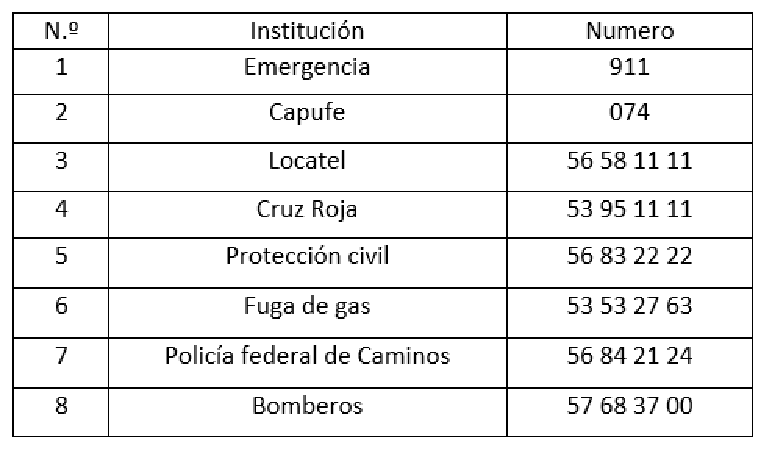
\includegraphics[scale=0.25]{30/img/numerosDeEmergencia.pdf}
        \caption{Identificación de los puntos de reunión dentro de la escuela}
        % \label{fig:my_label}
    \end{figure}
    
    % 
    % 
    % 
    % 
    \subsection{Análisis de los métodos, materiales, herramientas e instalación utilizada en la ejecución del ensamble de un circuito electrónico}
    
    \subsubsection{Verificación}
    
    Costos de no calidad.
    % 
    % 
    \subsubsection{Desarrollo del sistema de tiempos predeterminado}
    \begin{figure}[H]
        \centering
        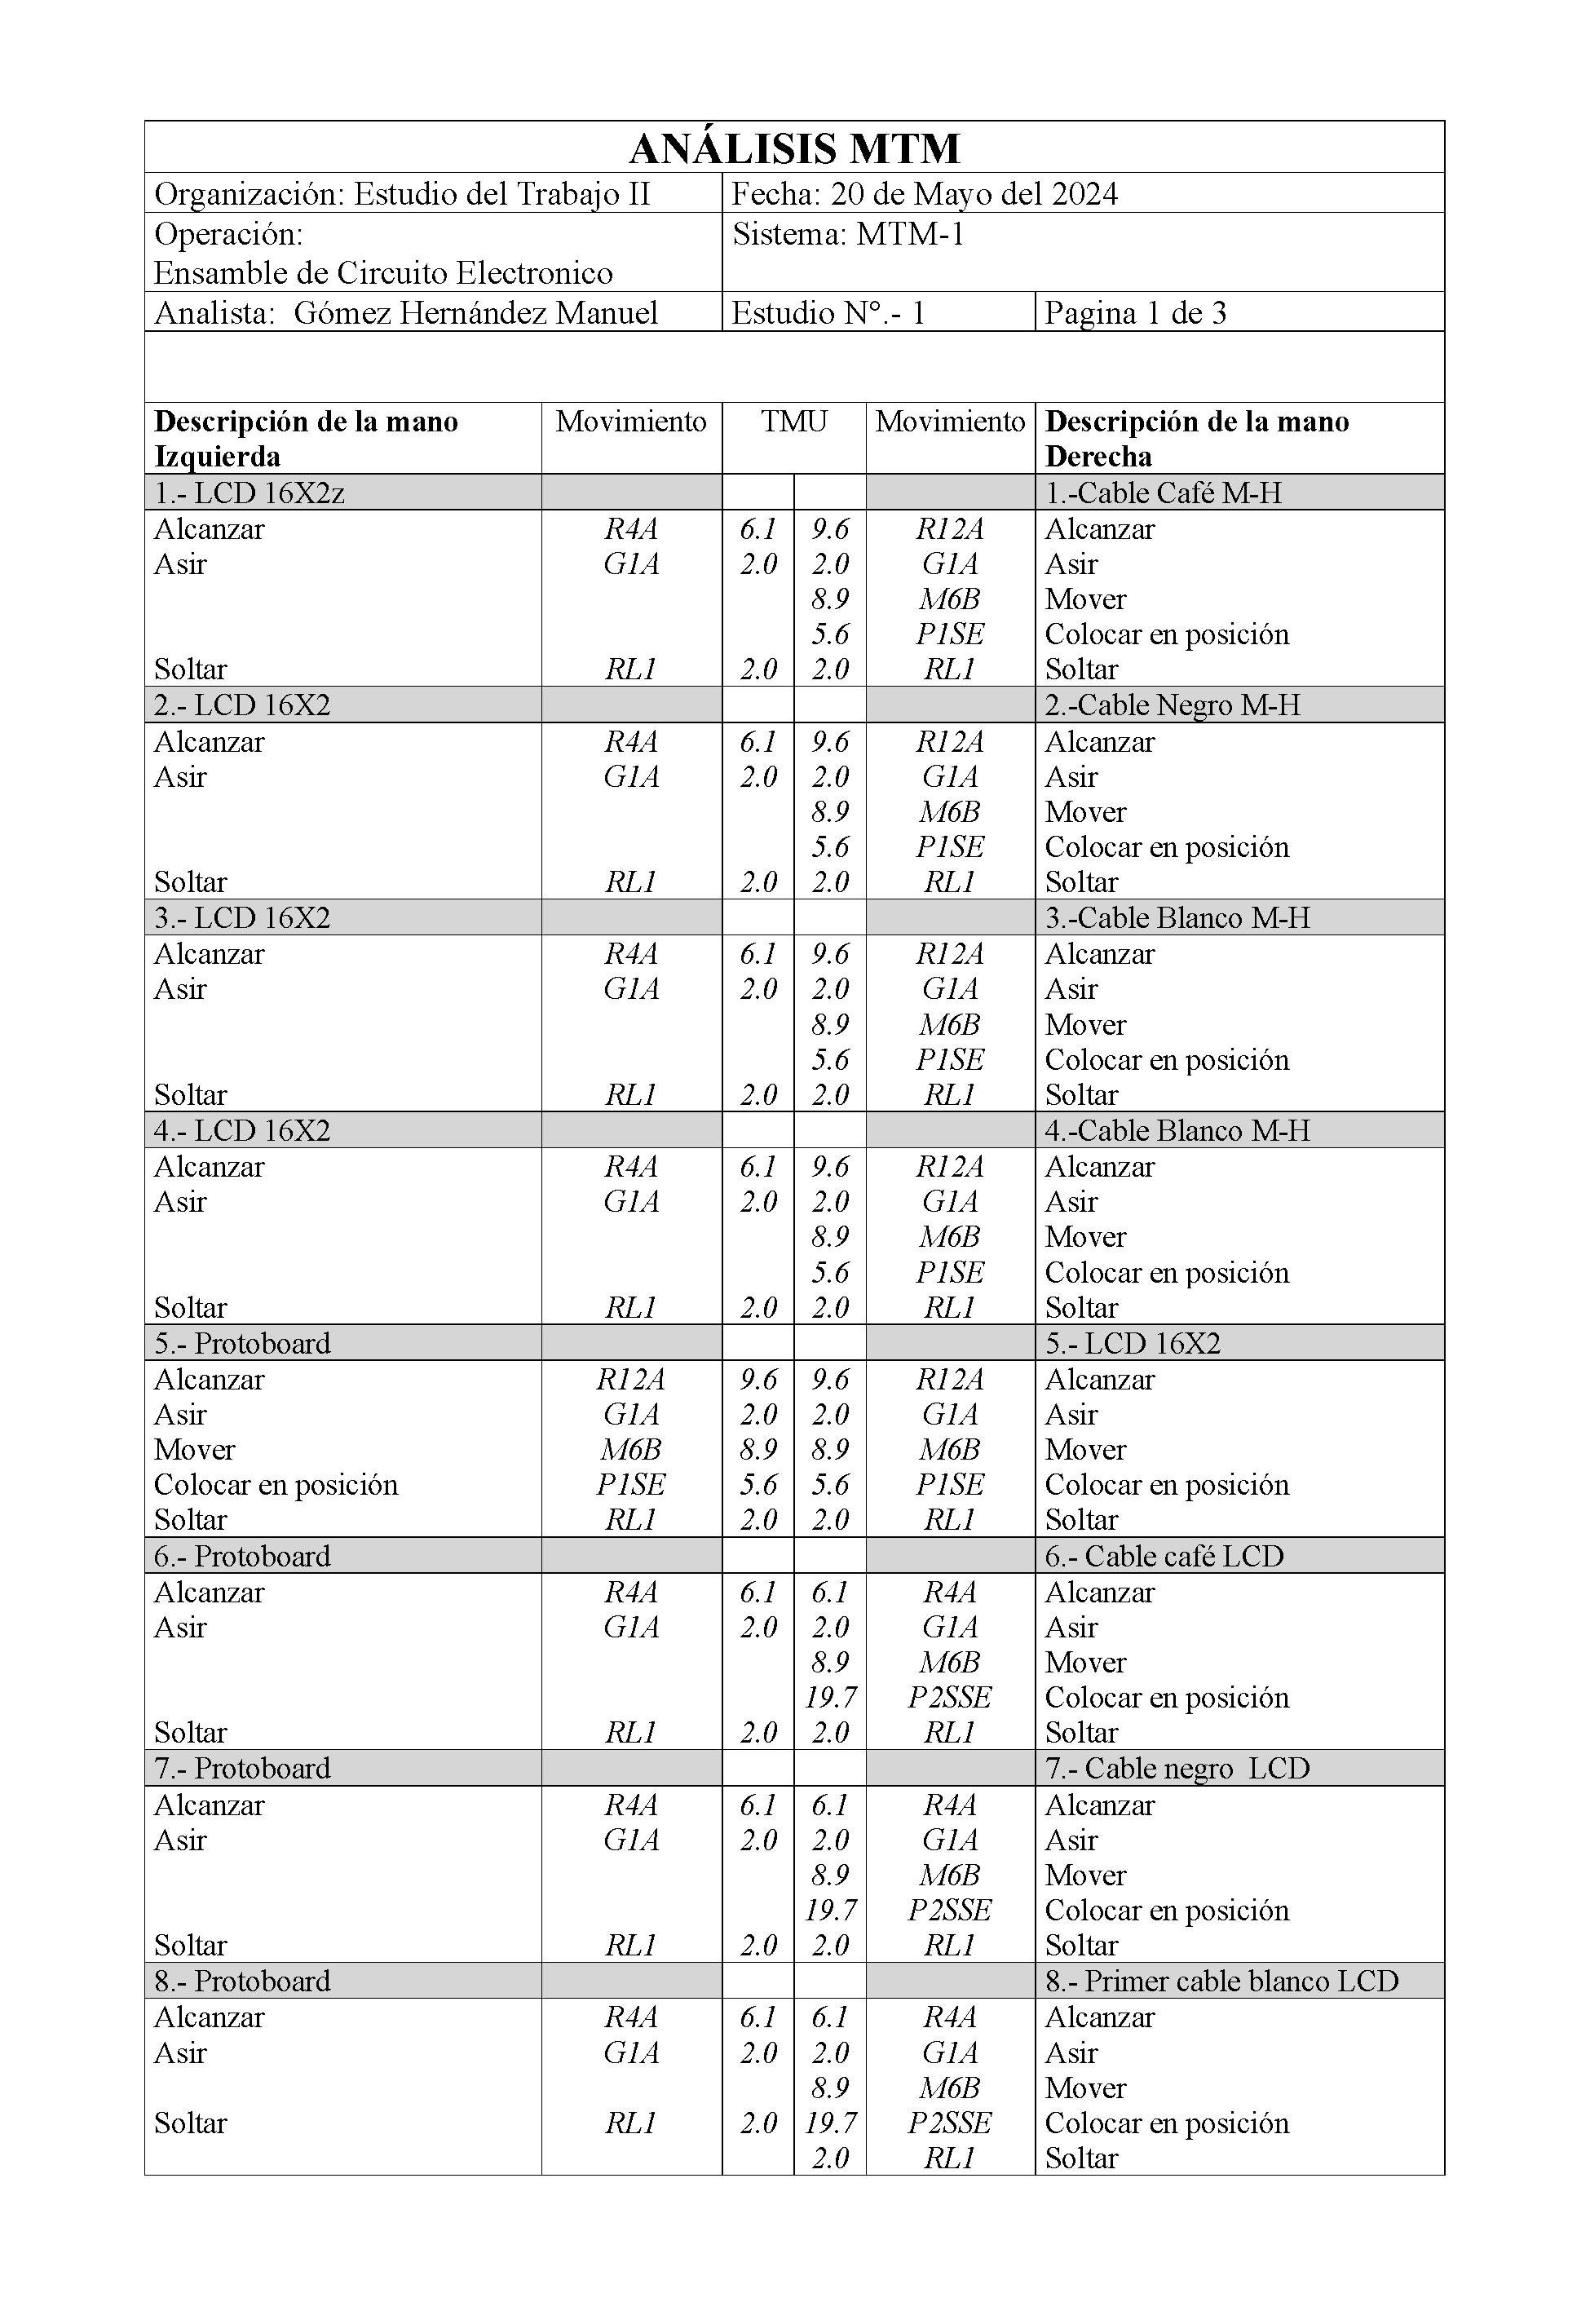
\includegraphics[scale=0.15]{30/img/tablaMTM1-1.pdf}
        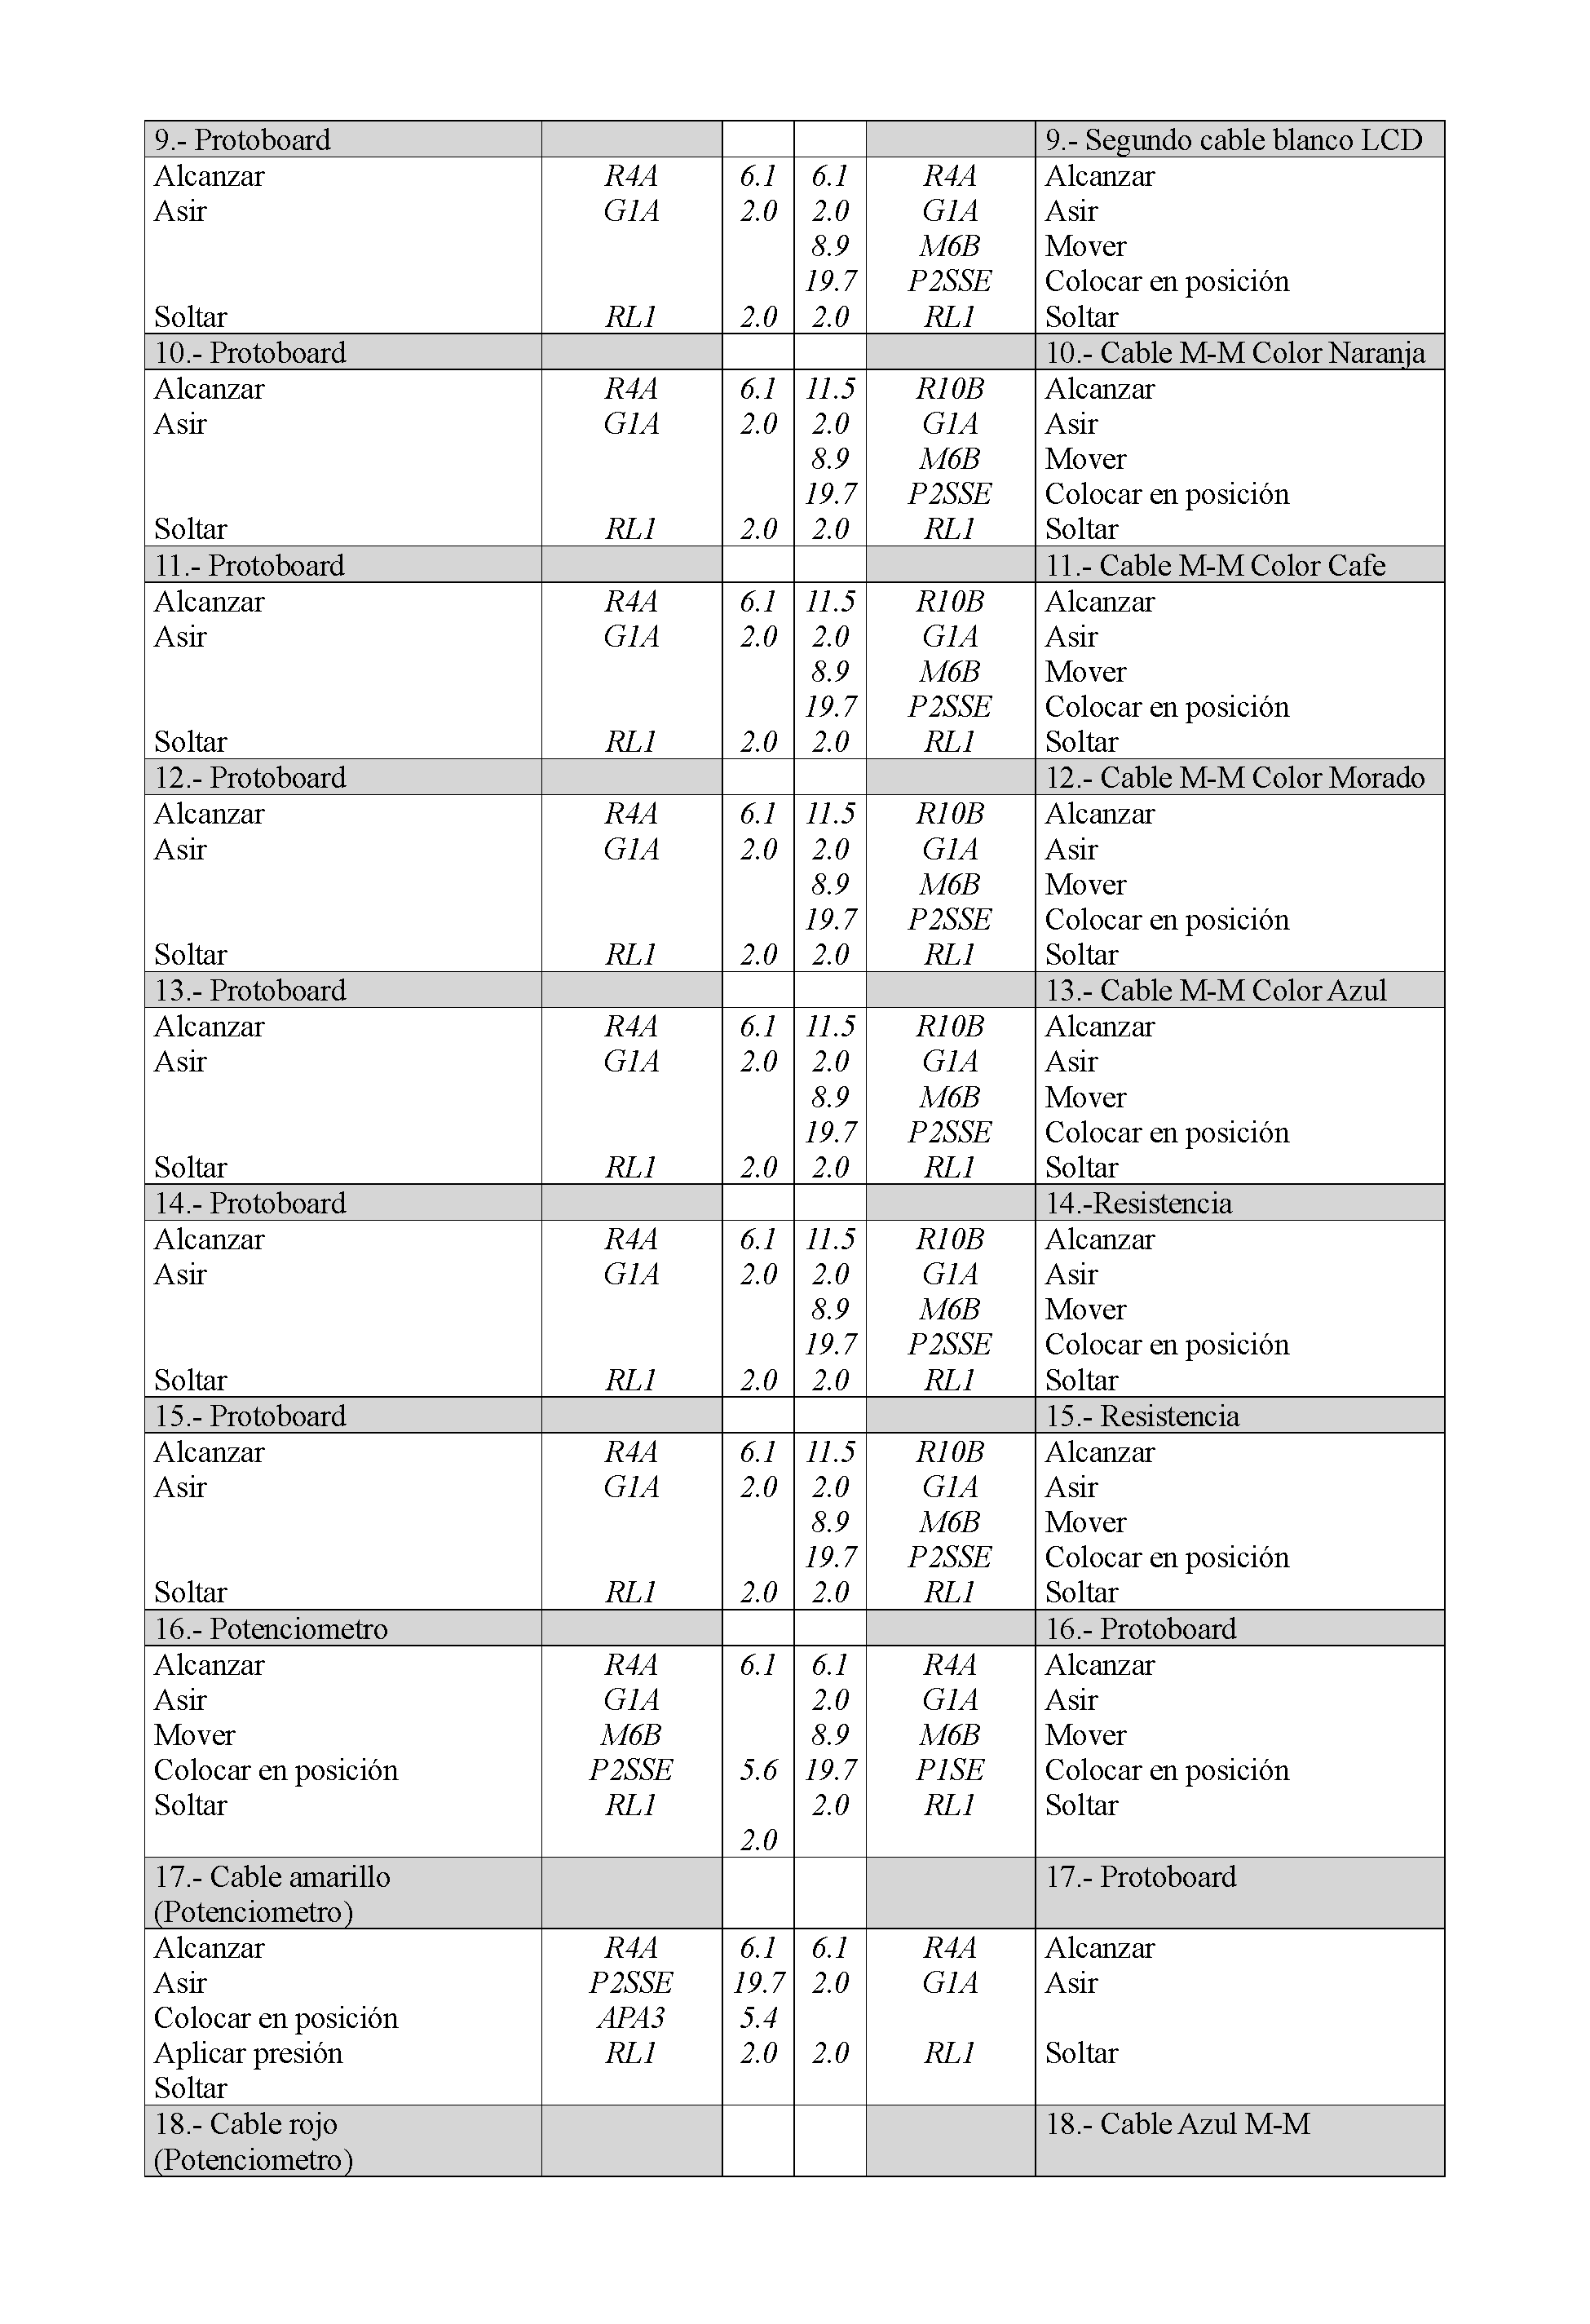
\includegraphics[scale=0.15]{30/img/tablaMTM1-2.pdf}
        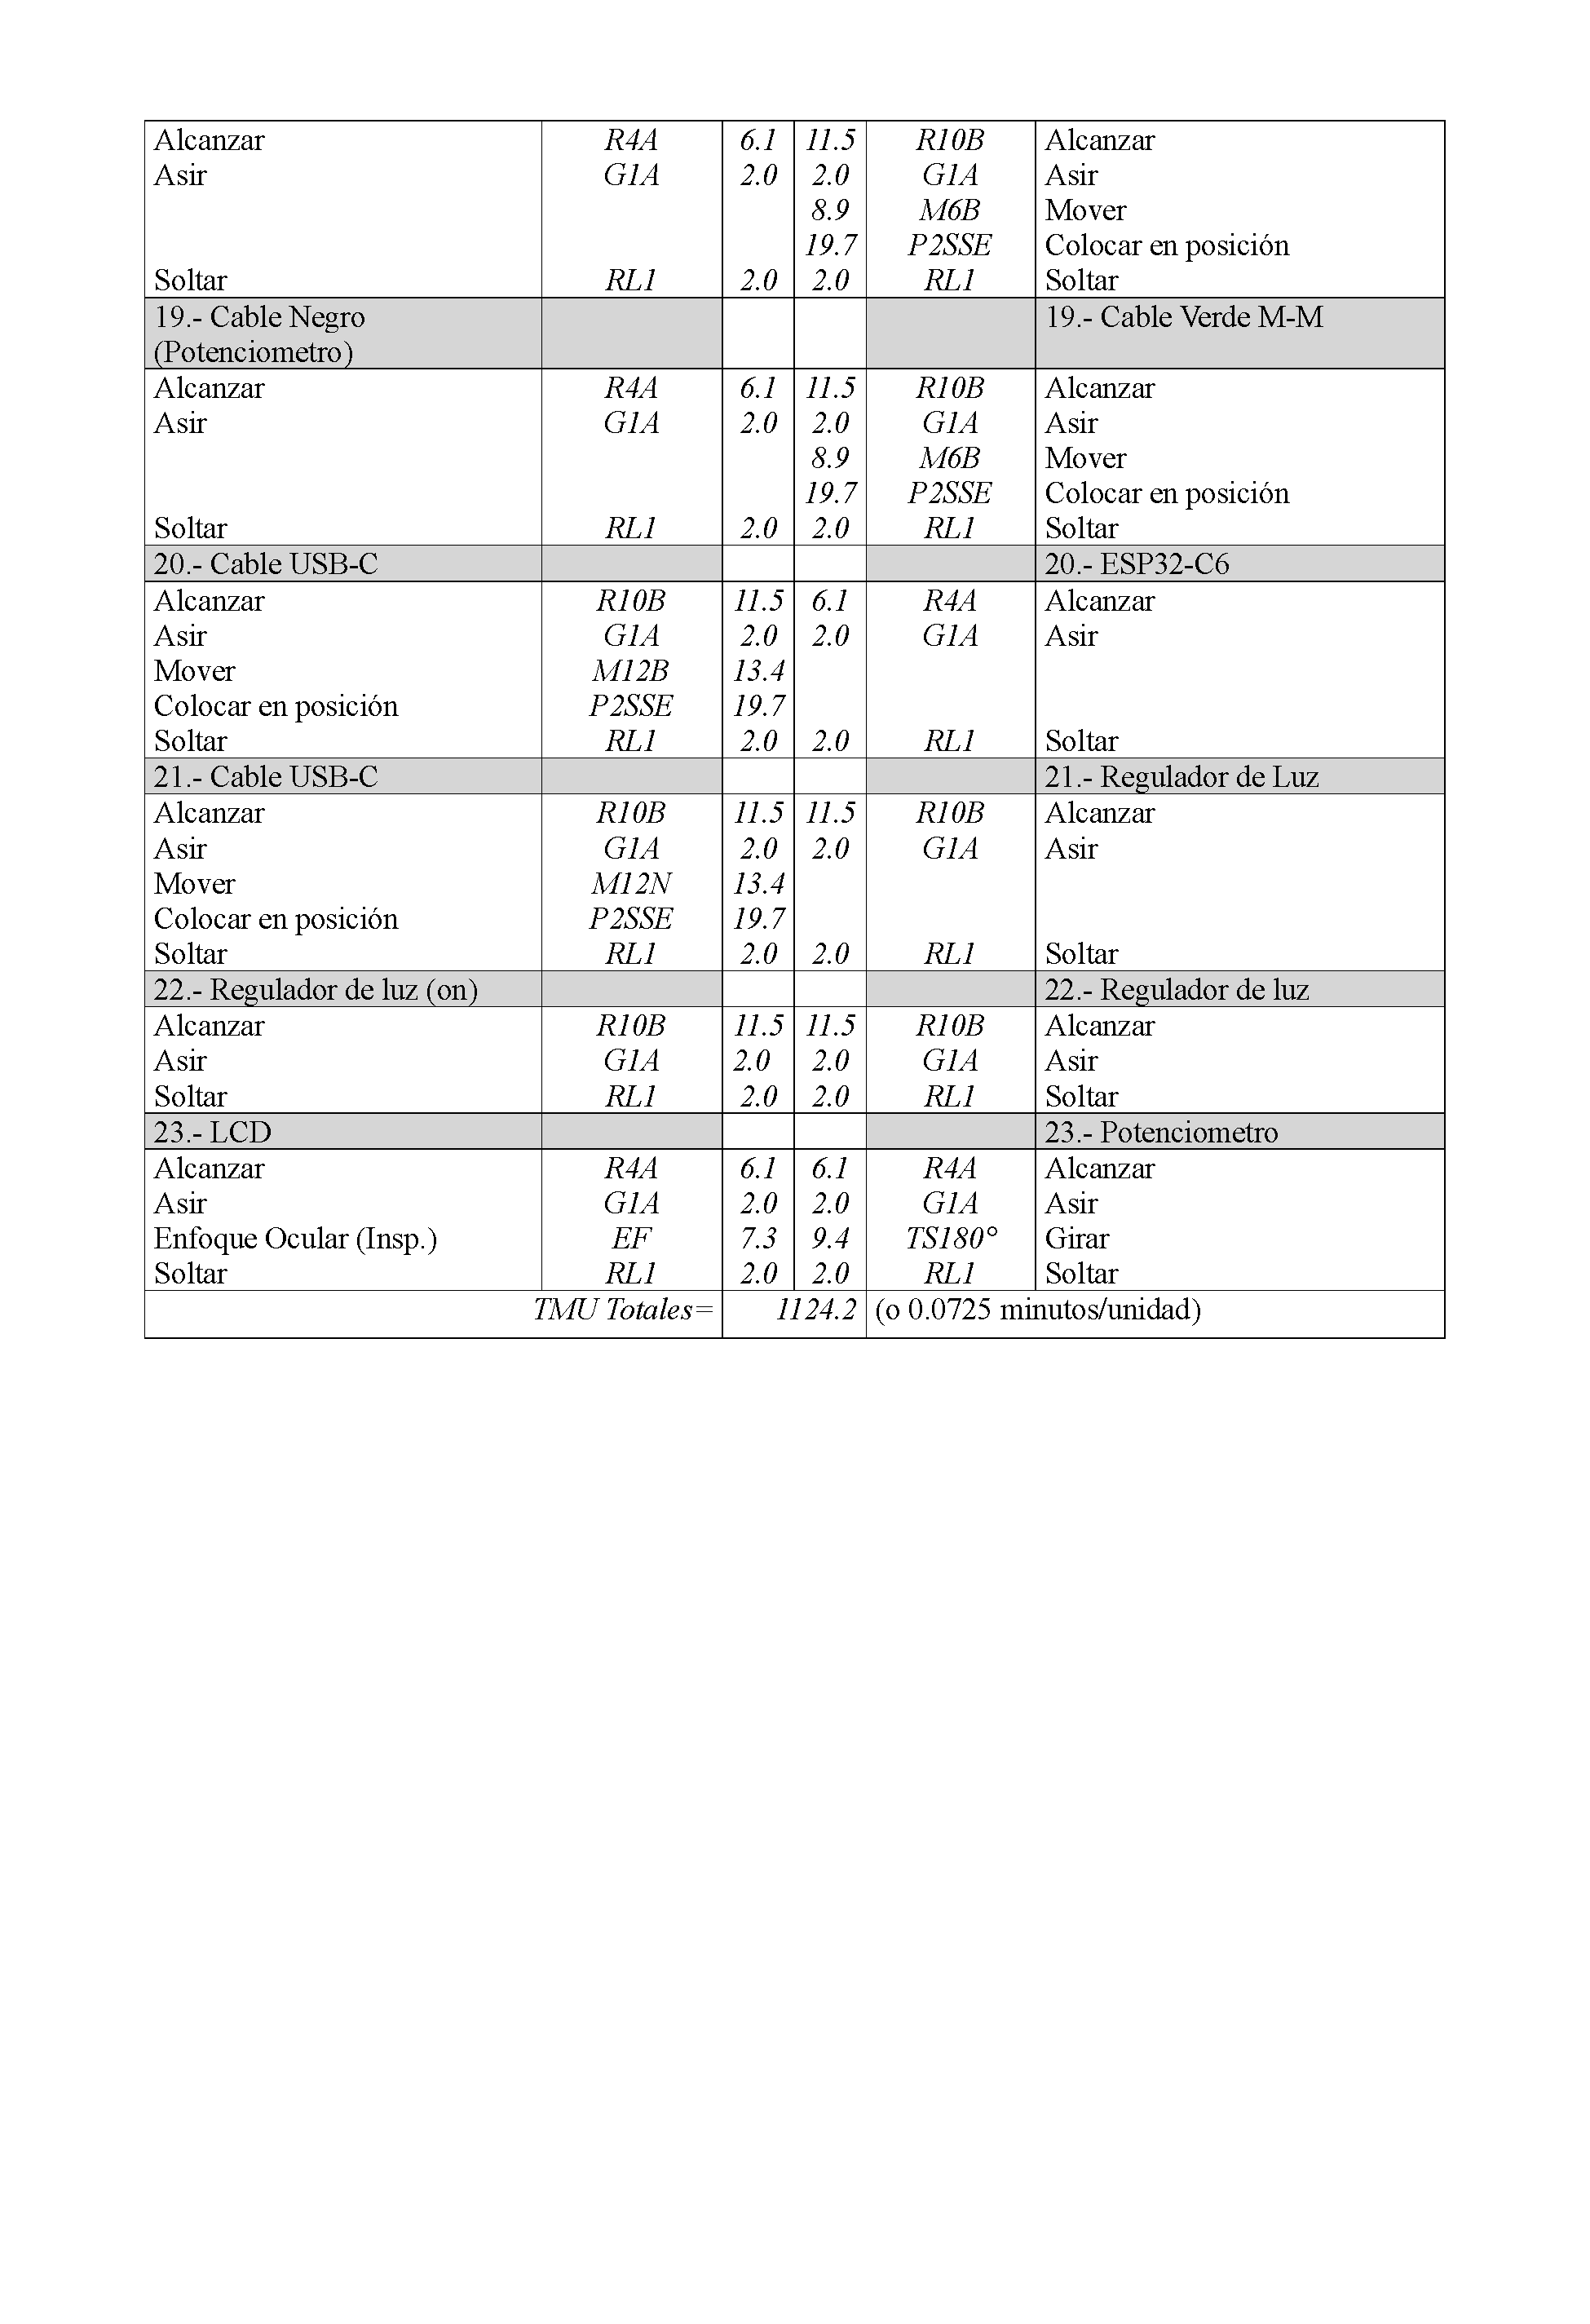
\includegraphics[scale=0.15]{30/img/tablaMTM1-3.pdf}
        \caption{Tablas MTM}
         \label{fig:tablasMTM}
    \end{figure}
    % 
    % 
    \subsubsection{Desarrollo del muestreo del trabajo}
    % 
    % 
    \subsubsection{Corrección por balanceo de procesos}
    % 
    % 
    \subsubsection{Datos estándar continuos y discretos}
    % 
    % 
    \subsection{Diseño de la forma más económica de realizar el trabajo}
    
    % 
    % 
    \subsection{Normalización de los métodos, materiales, herramientas e instalaciones}
    
    % 
    % 
    \subsection{Determinación del tiempo estándar para que una persona competente realice el trabajo con marcha normal}
    \begin{figure}[H]
        \centering
        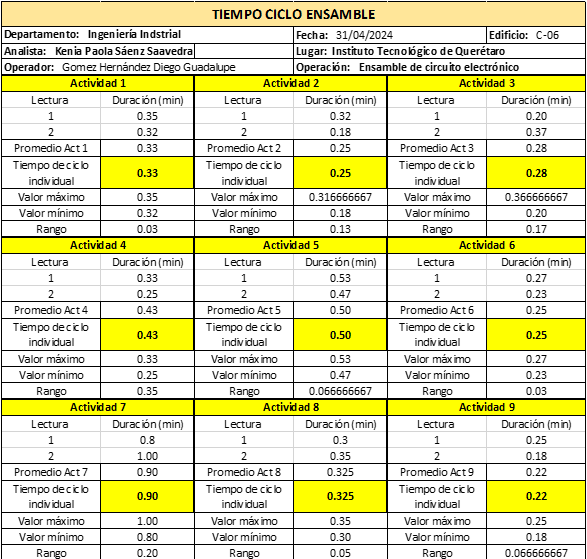
\includegraphics[scale=0.25]{30/img/tiempoCiclo1.pdf}
        \label{fig:tiempoCiclo}
    \end{figure}
    \begin{figure}[H]
        \centering
        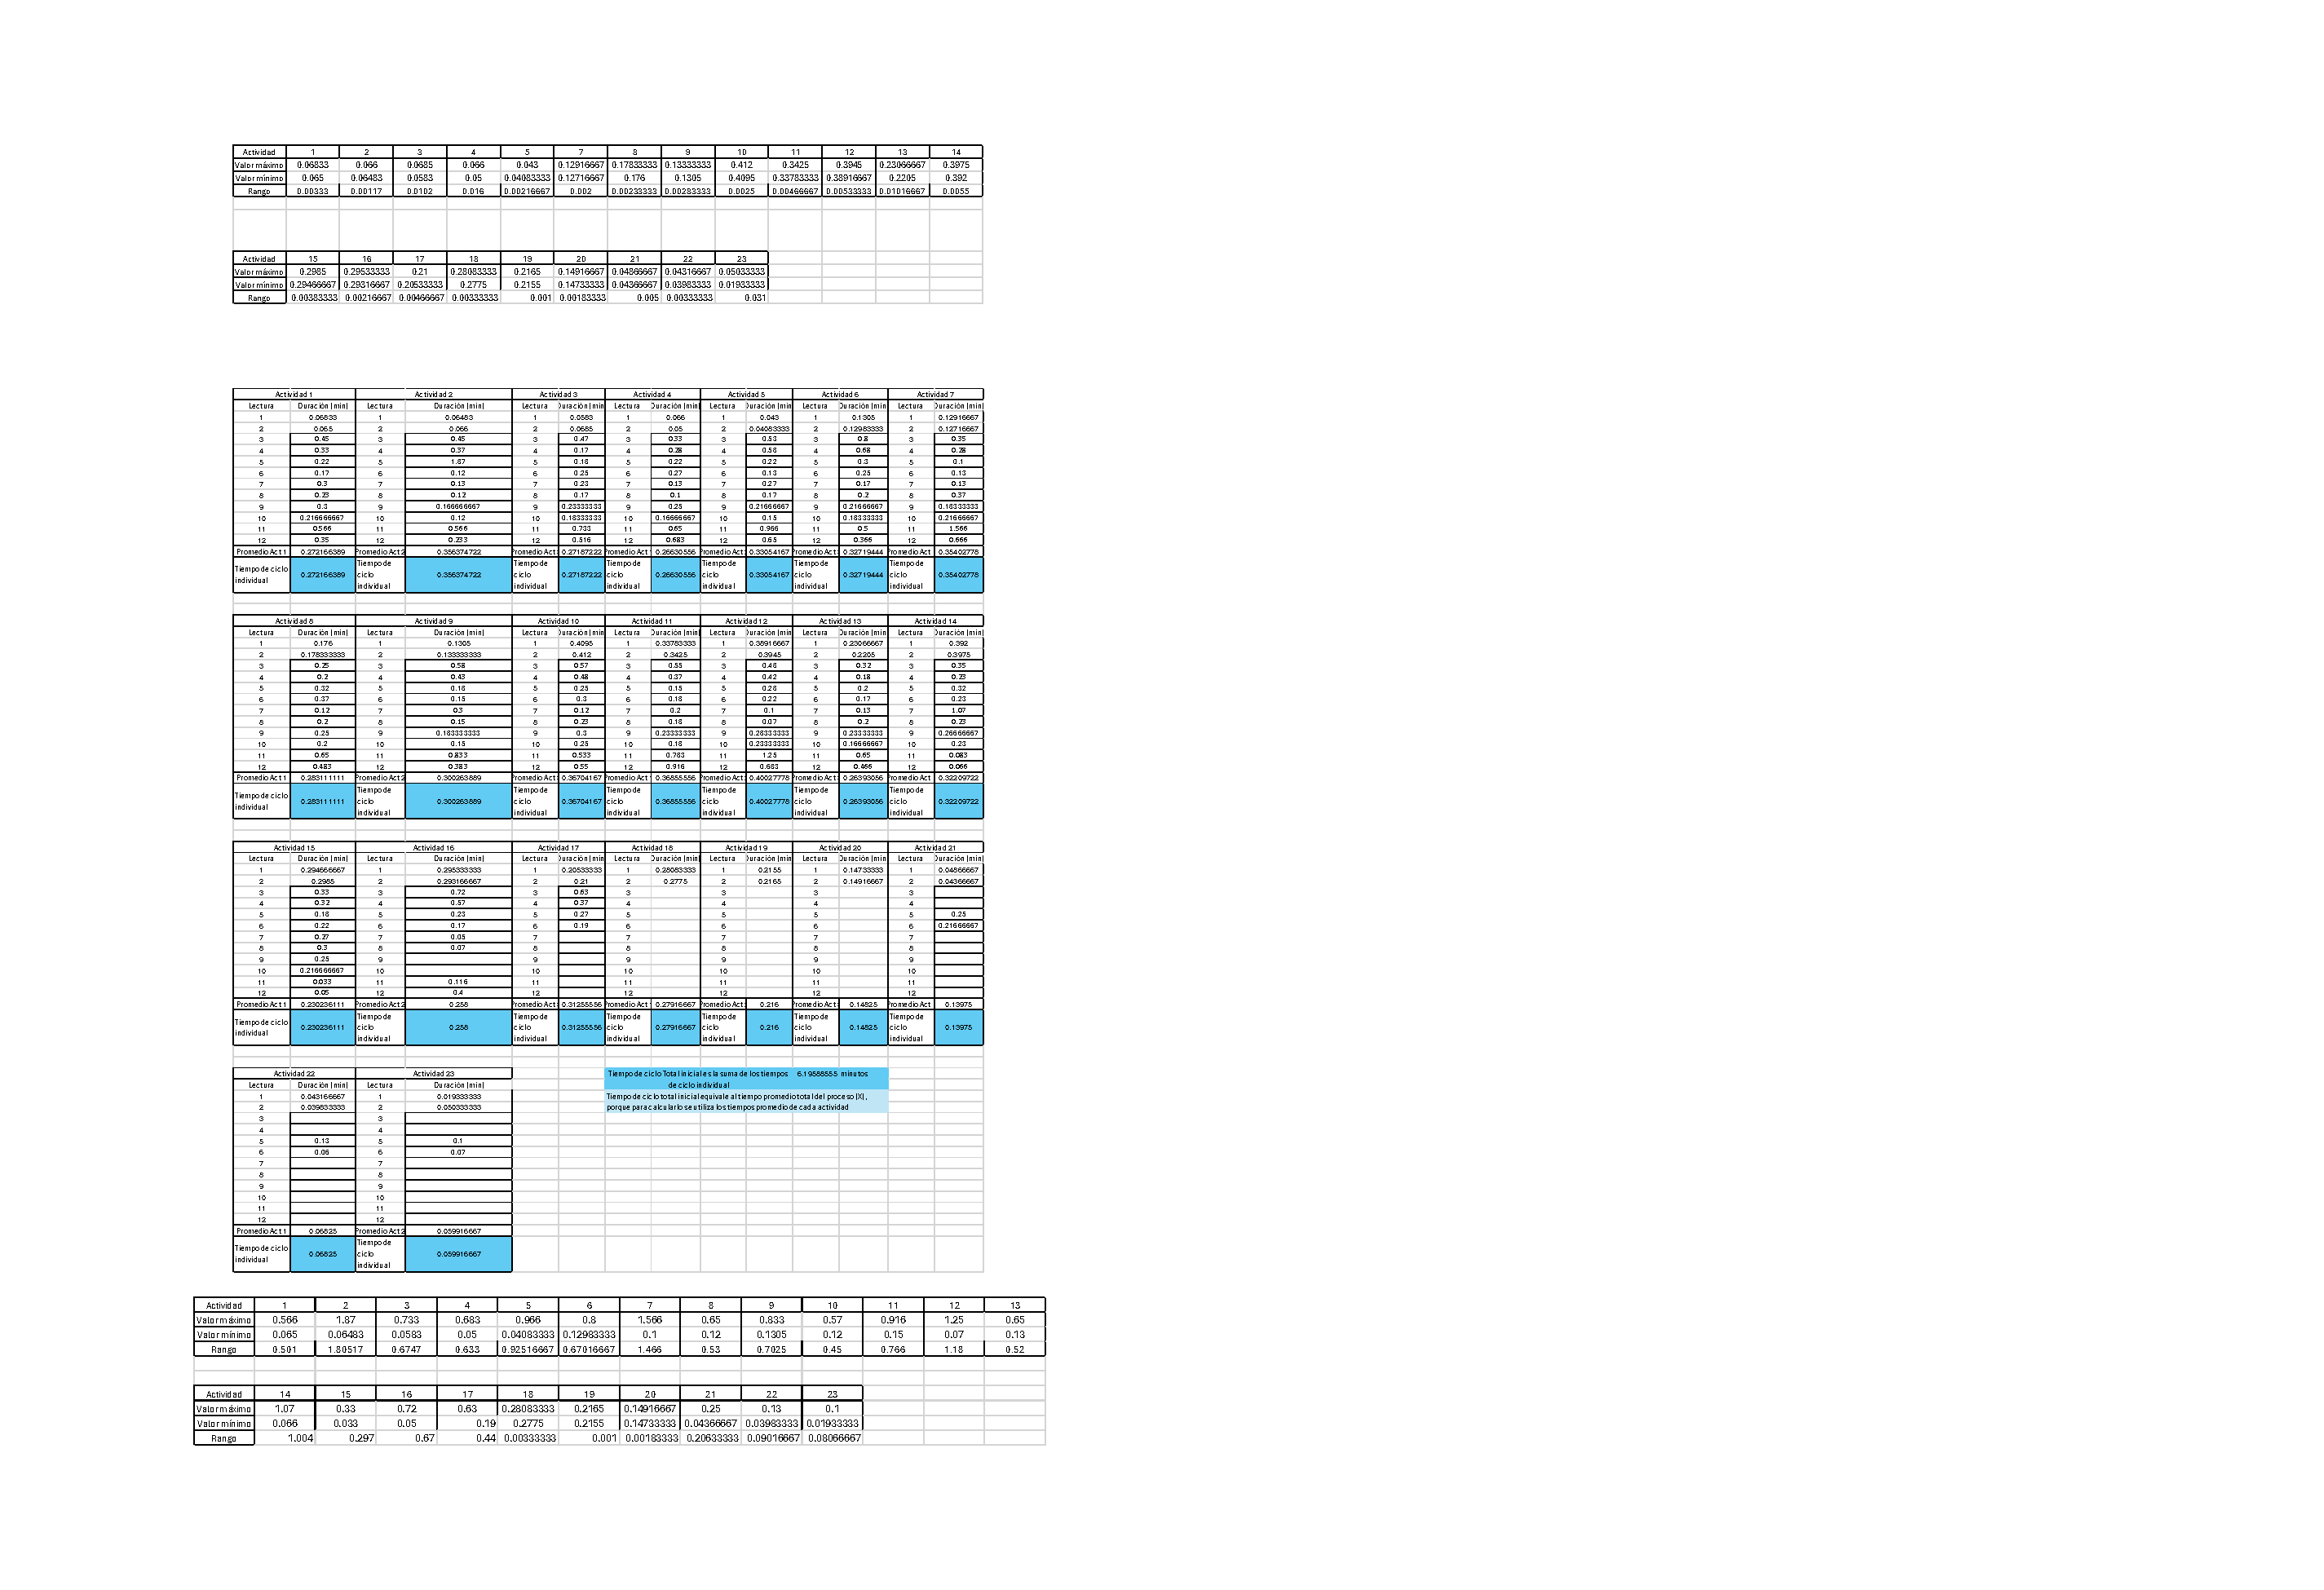
\includegraphics[scale=0.40]{30/img/tiempoCiclos2.pdf}
        \caption{Tablas de tiempo de ciclos}
        \label{fig:tiempoCiclo}
    \end{figure}
    \begin{figure}[H]
        \centering
        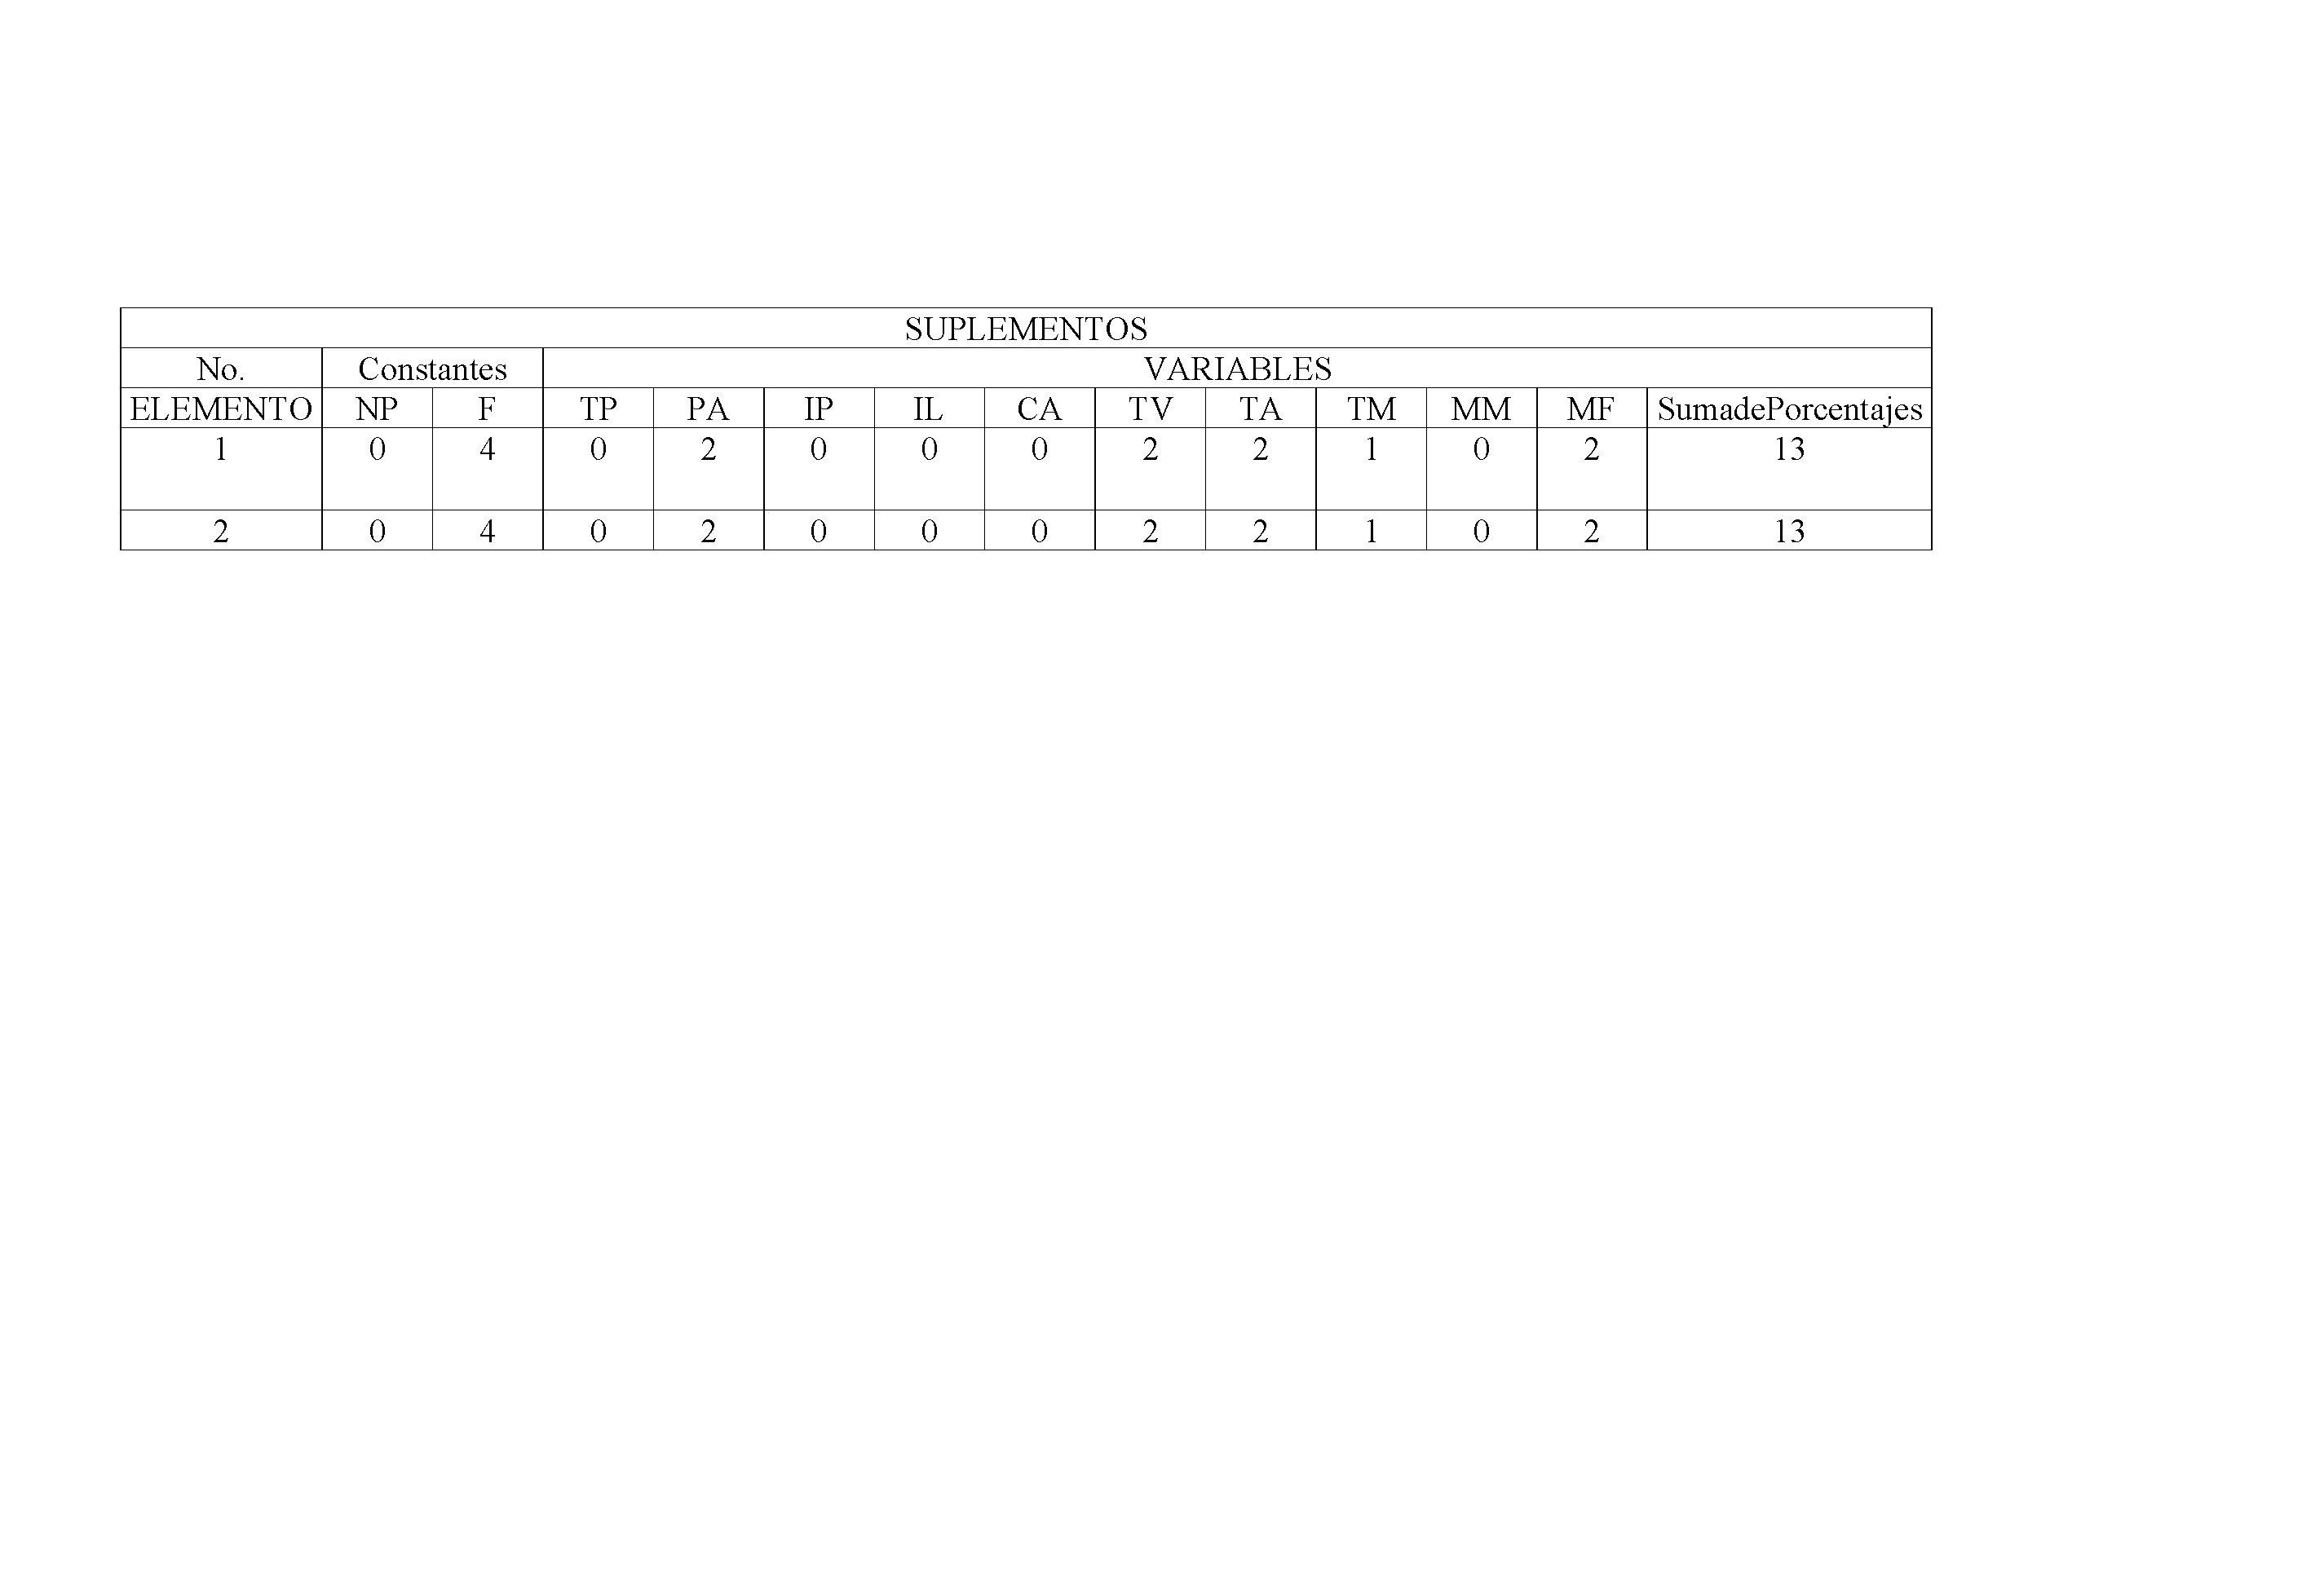
\includegraphics[scale=0.25]{30/img/determinacionHolguras.pdf}
        \caption{Tiempo estandar}
        \label{fig:deterholgura}
    \end{figure}
    
    \begin{figure}[H]
        \centering
        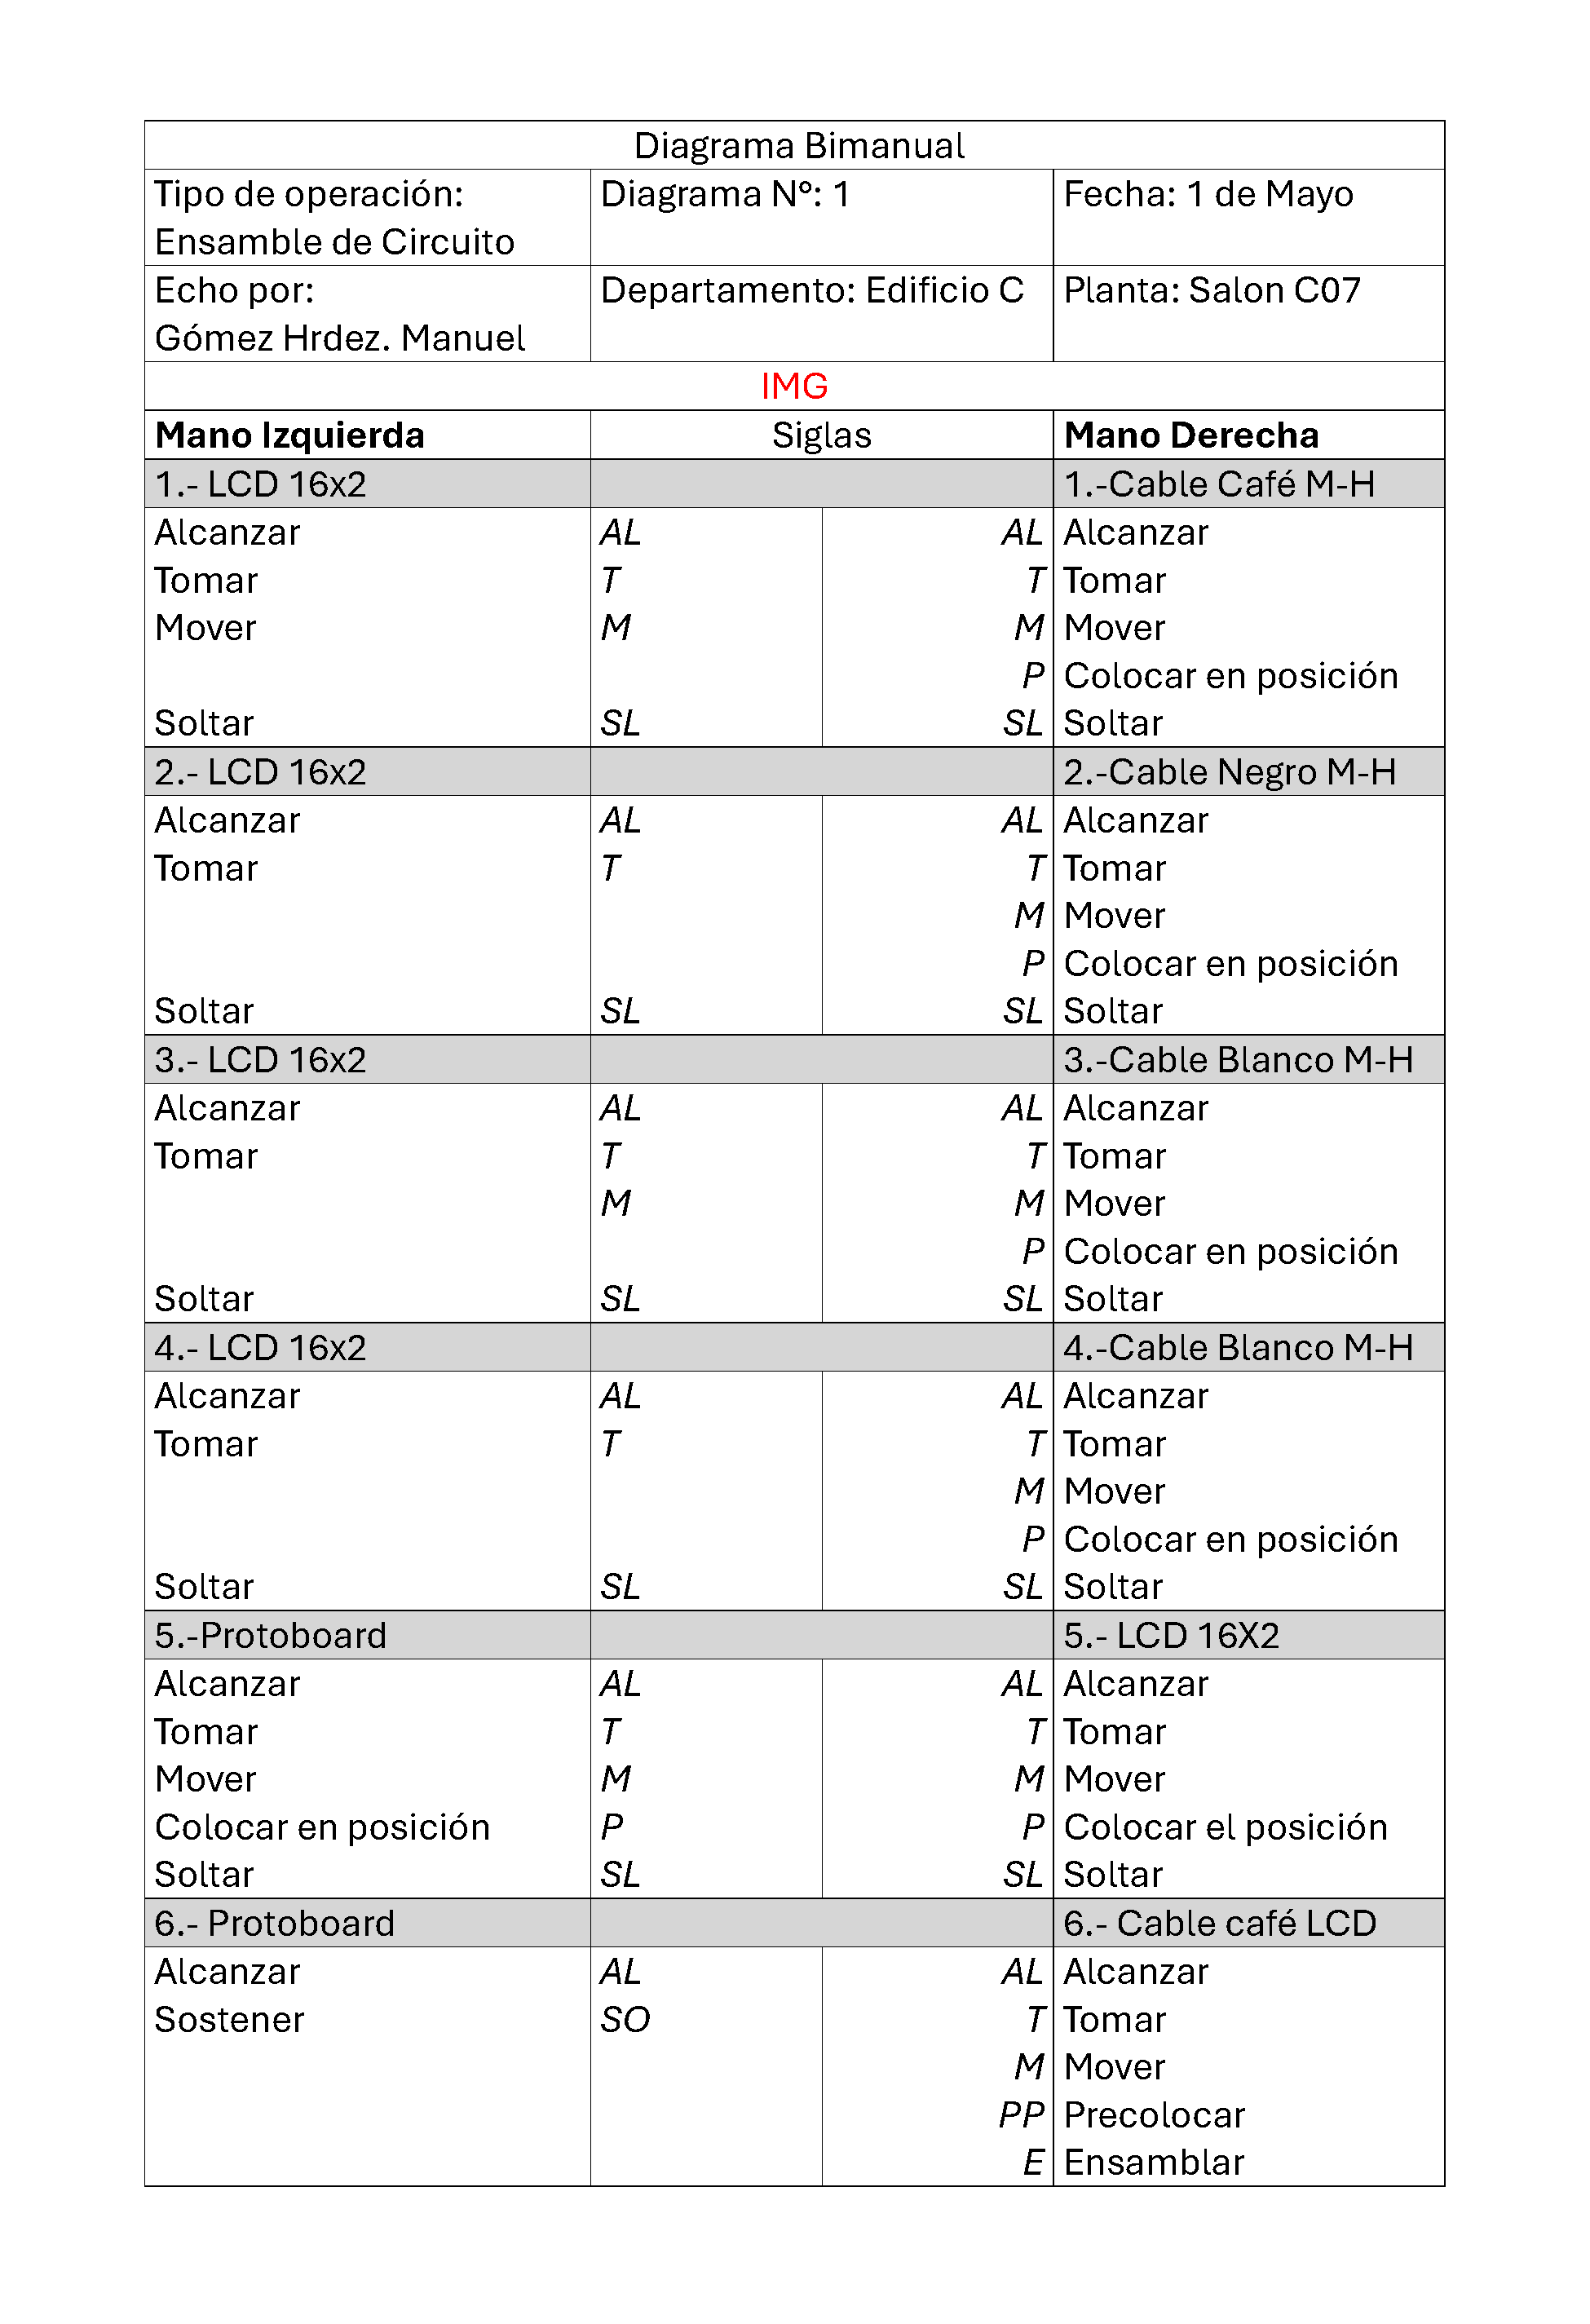
\includegraphics[scale=0.25]{30/img/diagramaBimanualEnsamble-1.pdf}
        % \label{fig:my_label}
    \end{figure}
    \begin{figure}[H]
        \centering
        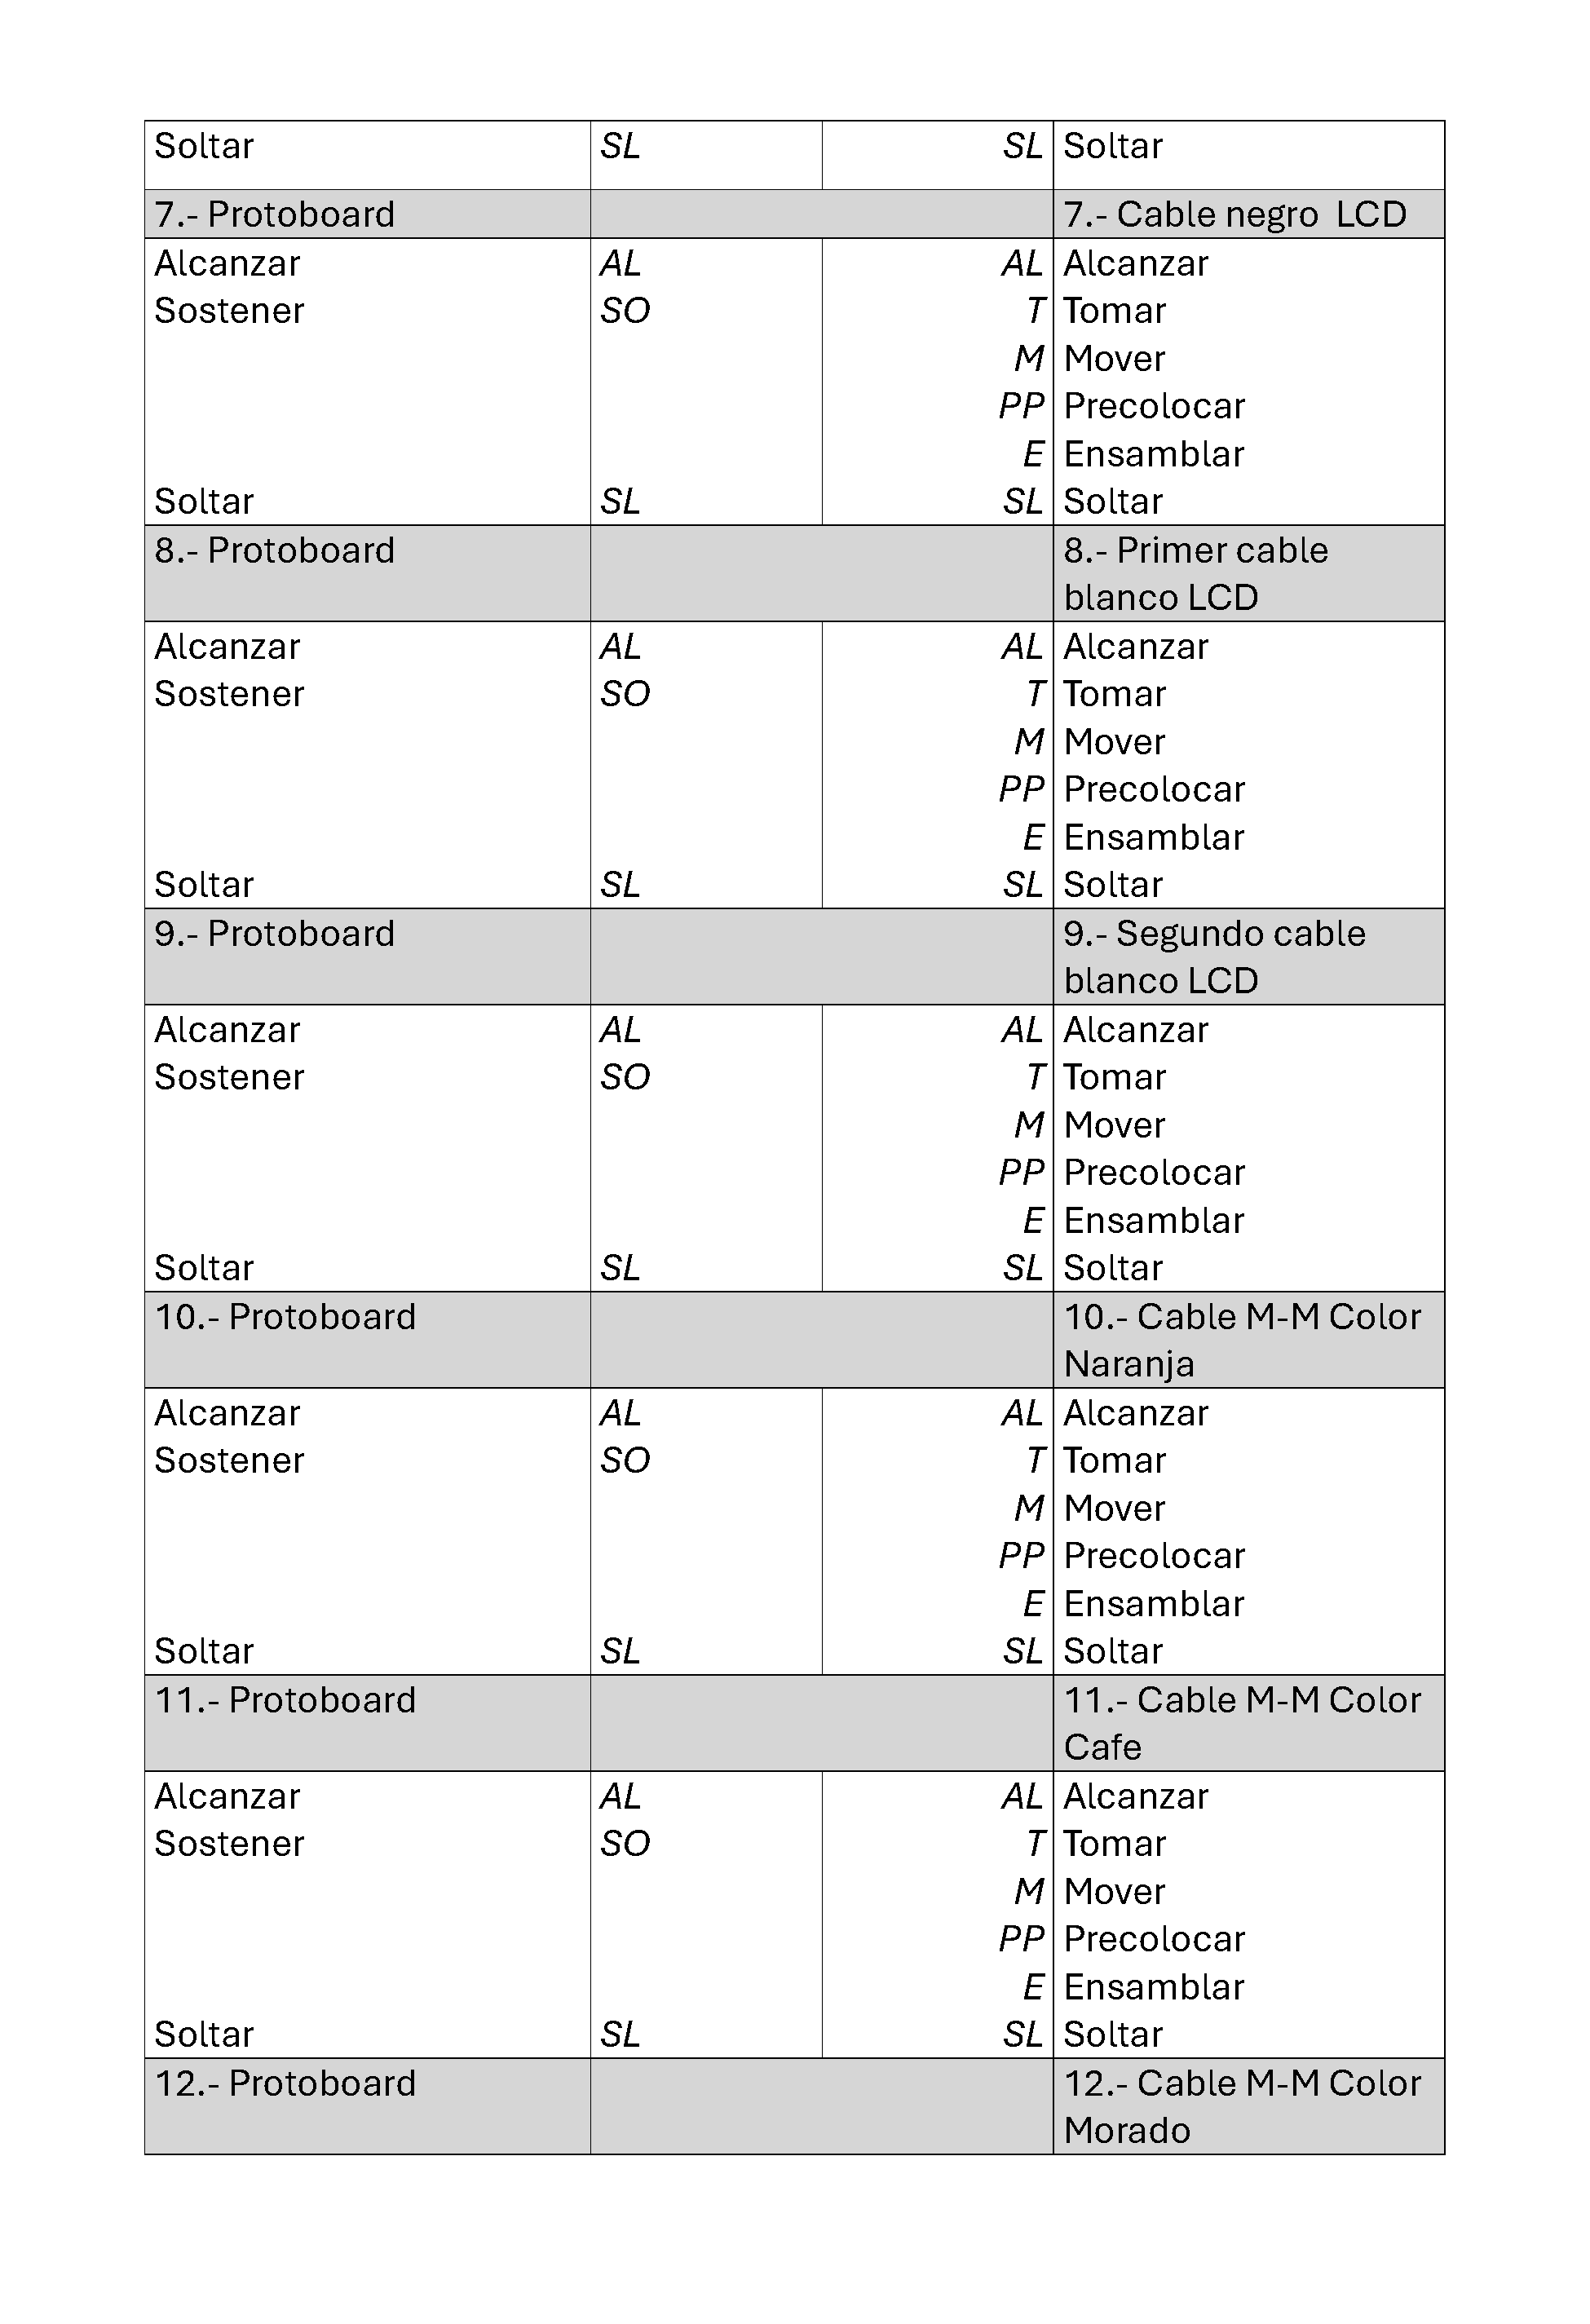
\includegraphics[scale=0.25]{30/img/diagramaBimanualEnsamble-2.pdf}
        % \label{fig:my_label}
    \end{figure}
    \begin{figure}[H]
        \centering
        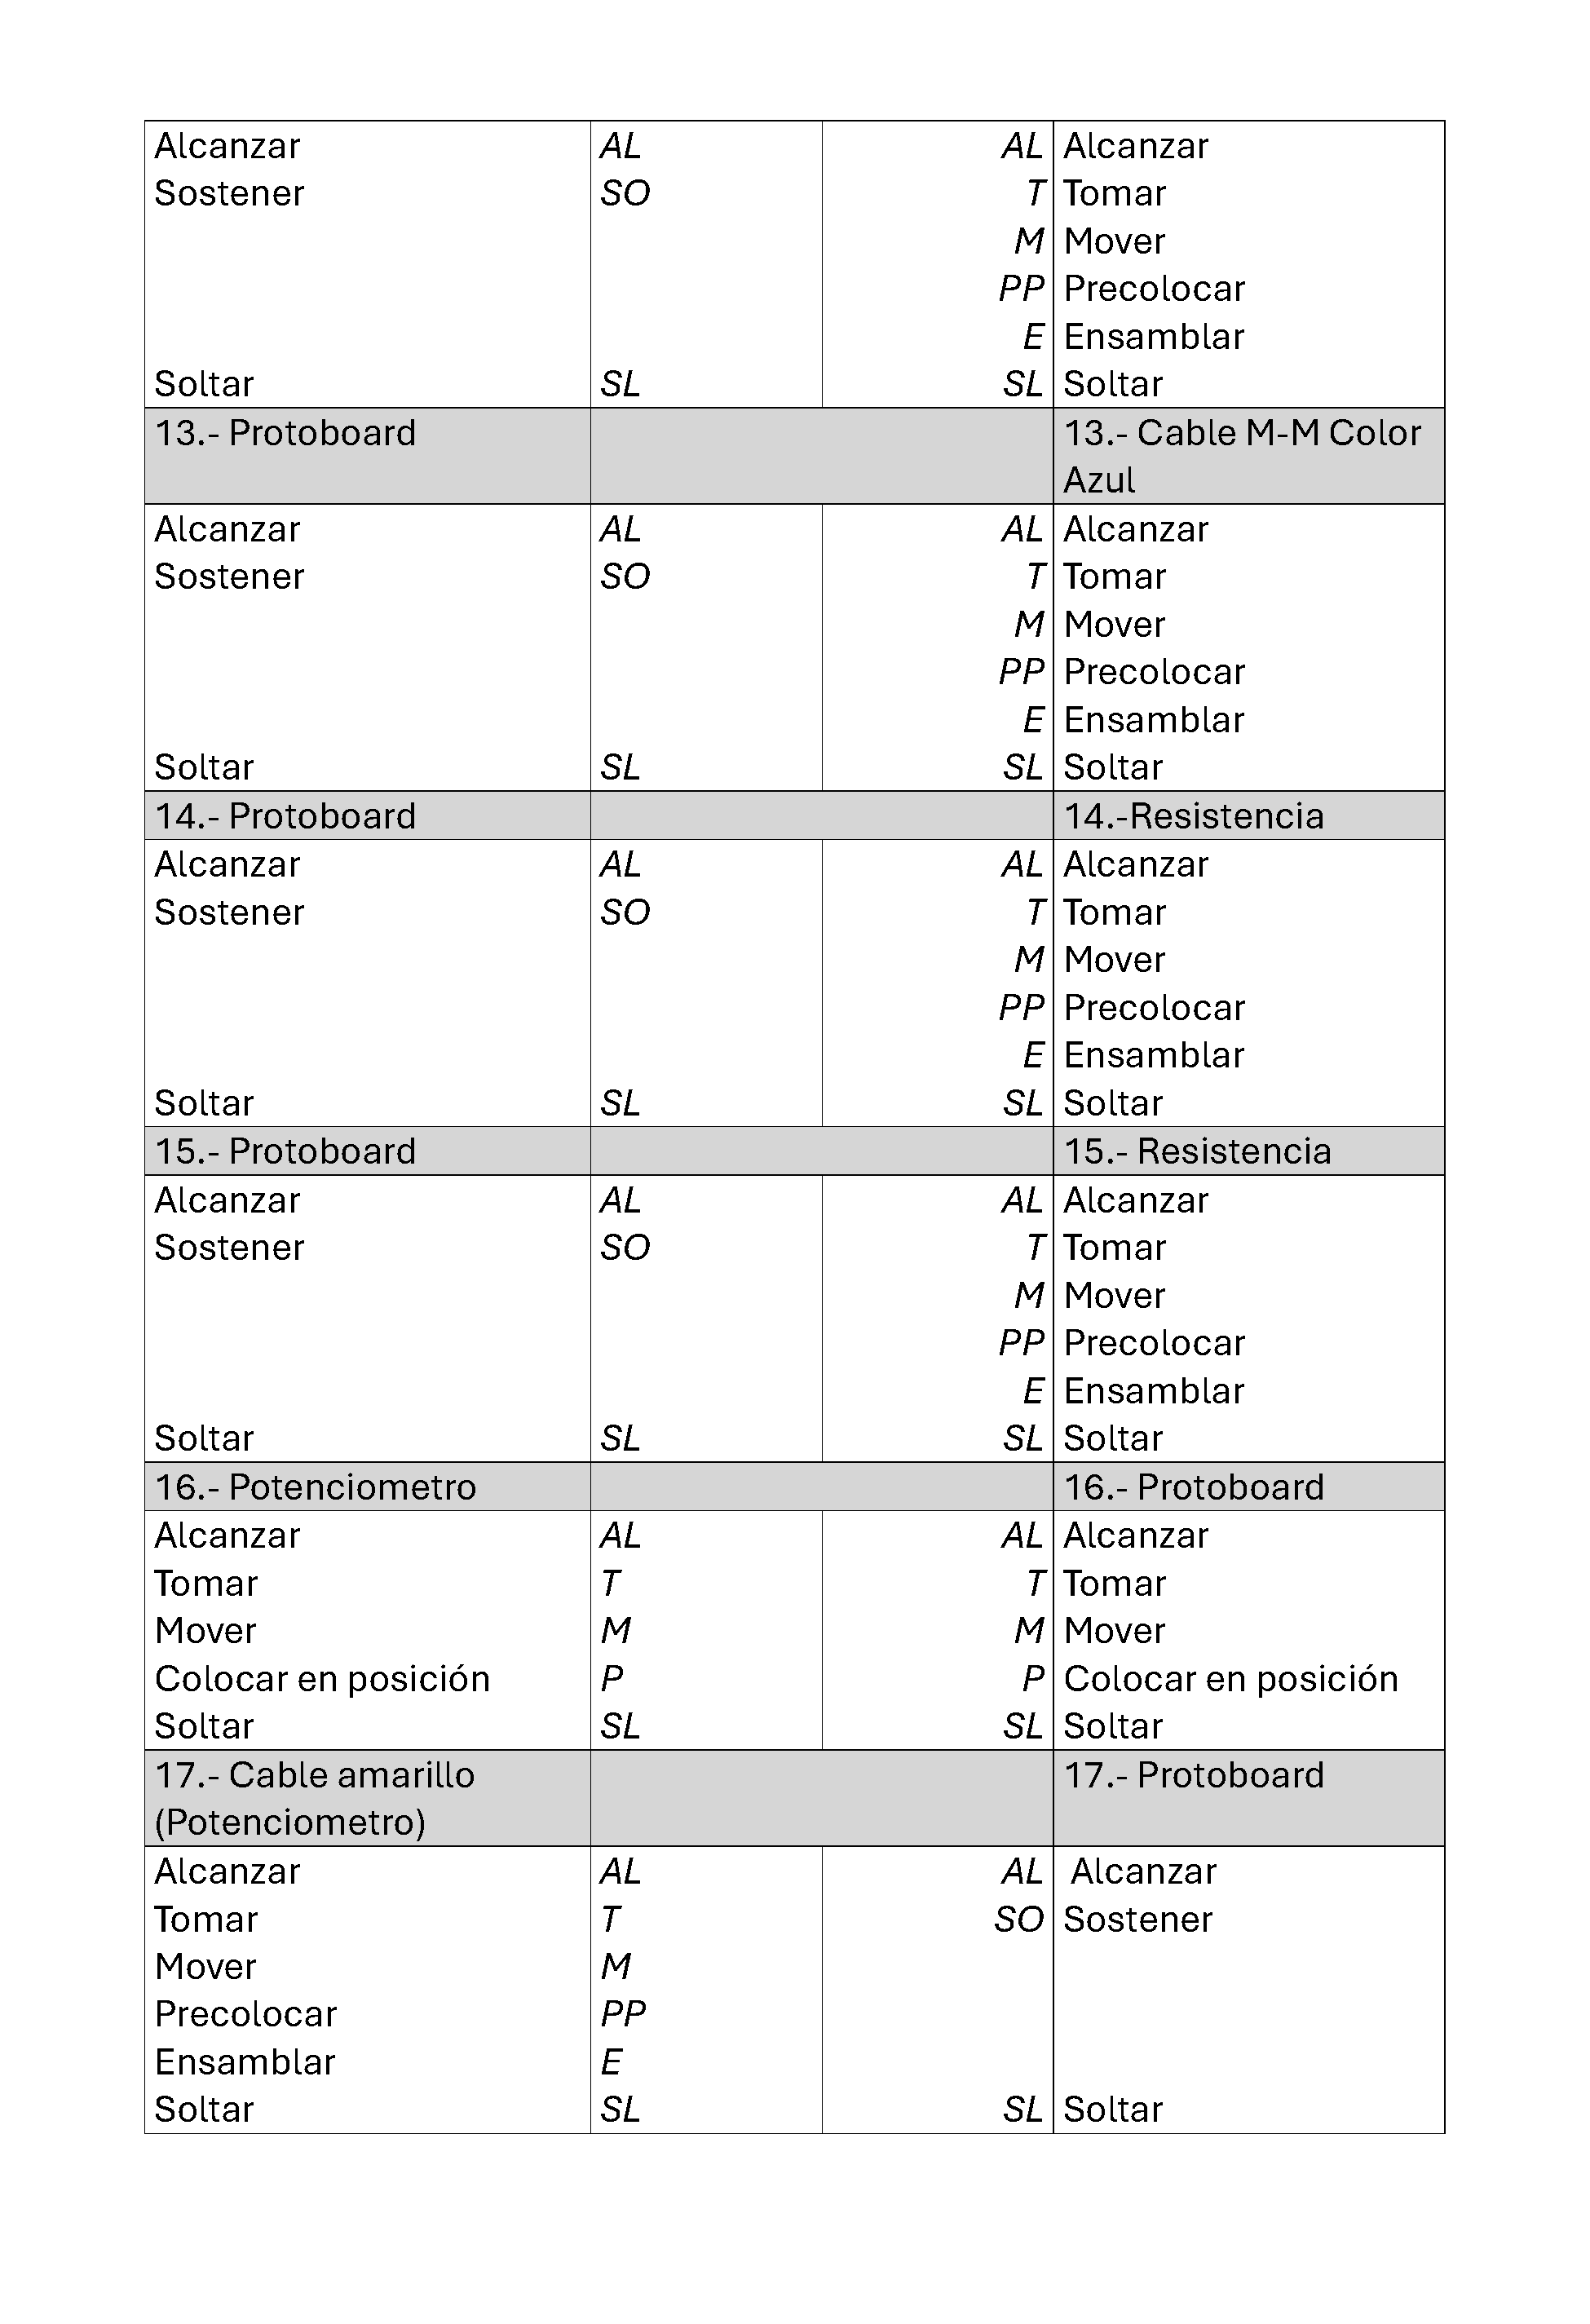
\includegraphics[scale=0.25]{30/img/diagramaBimanualEnsamble-3.pdf}
        % \label{fig:my_label}
    \end{figure}
    \begin{figure}[H]
        \centering
        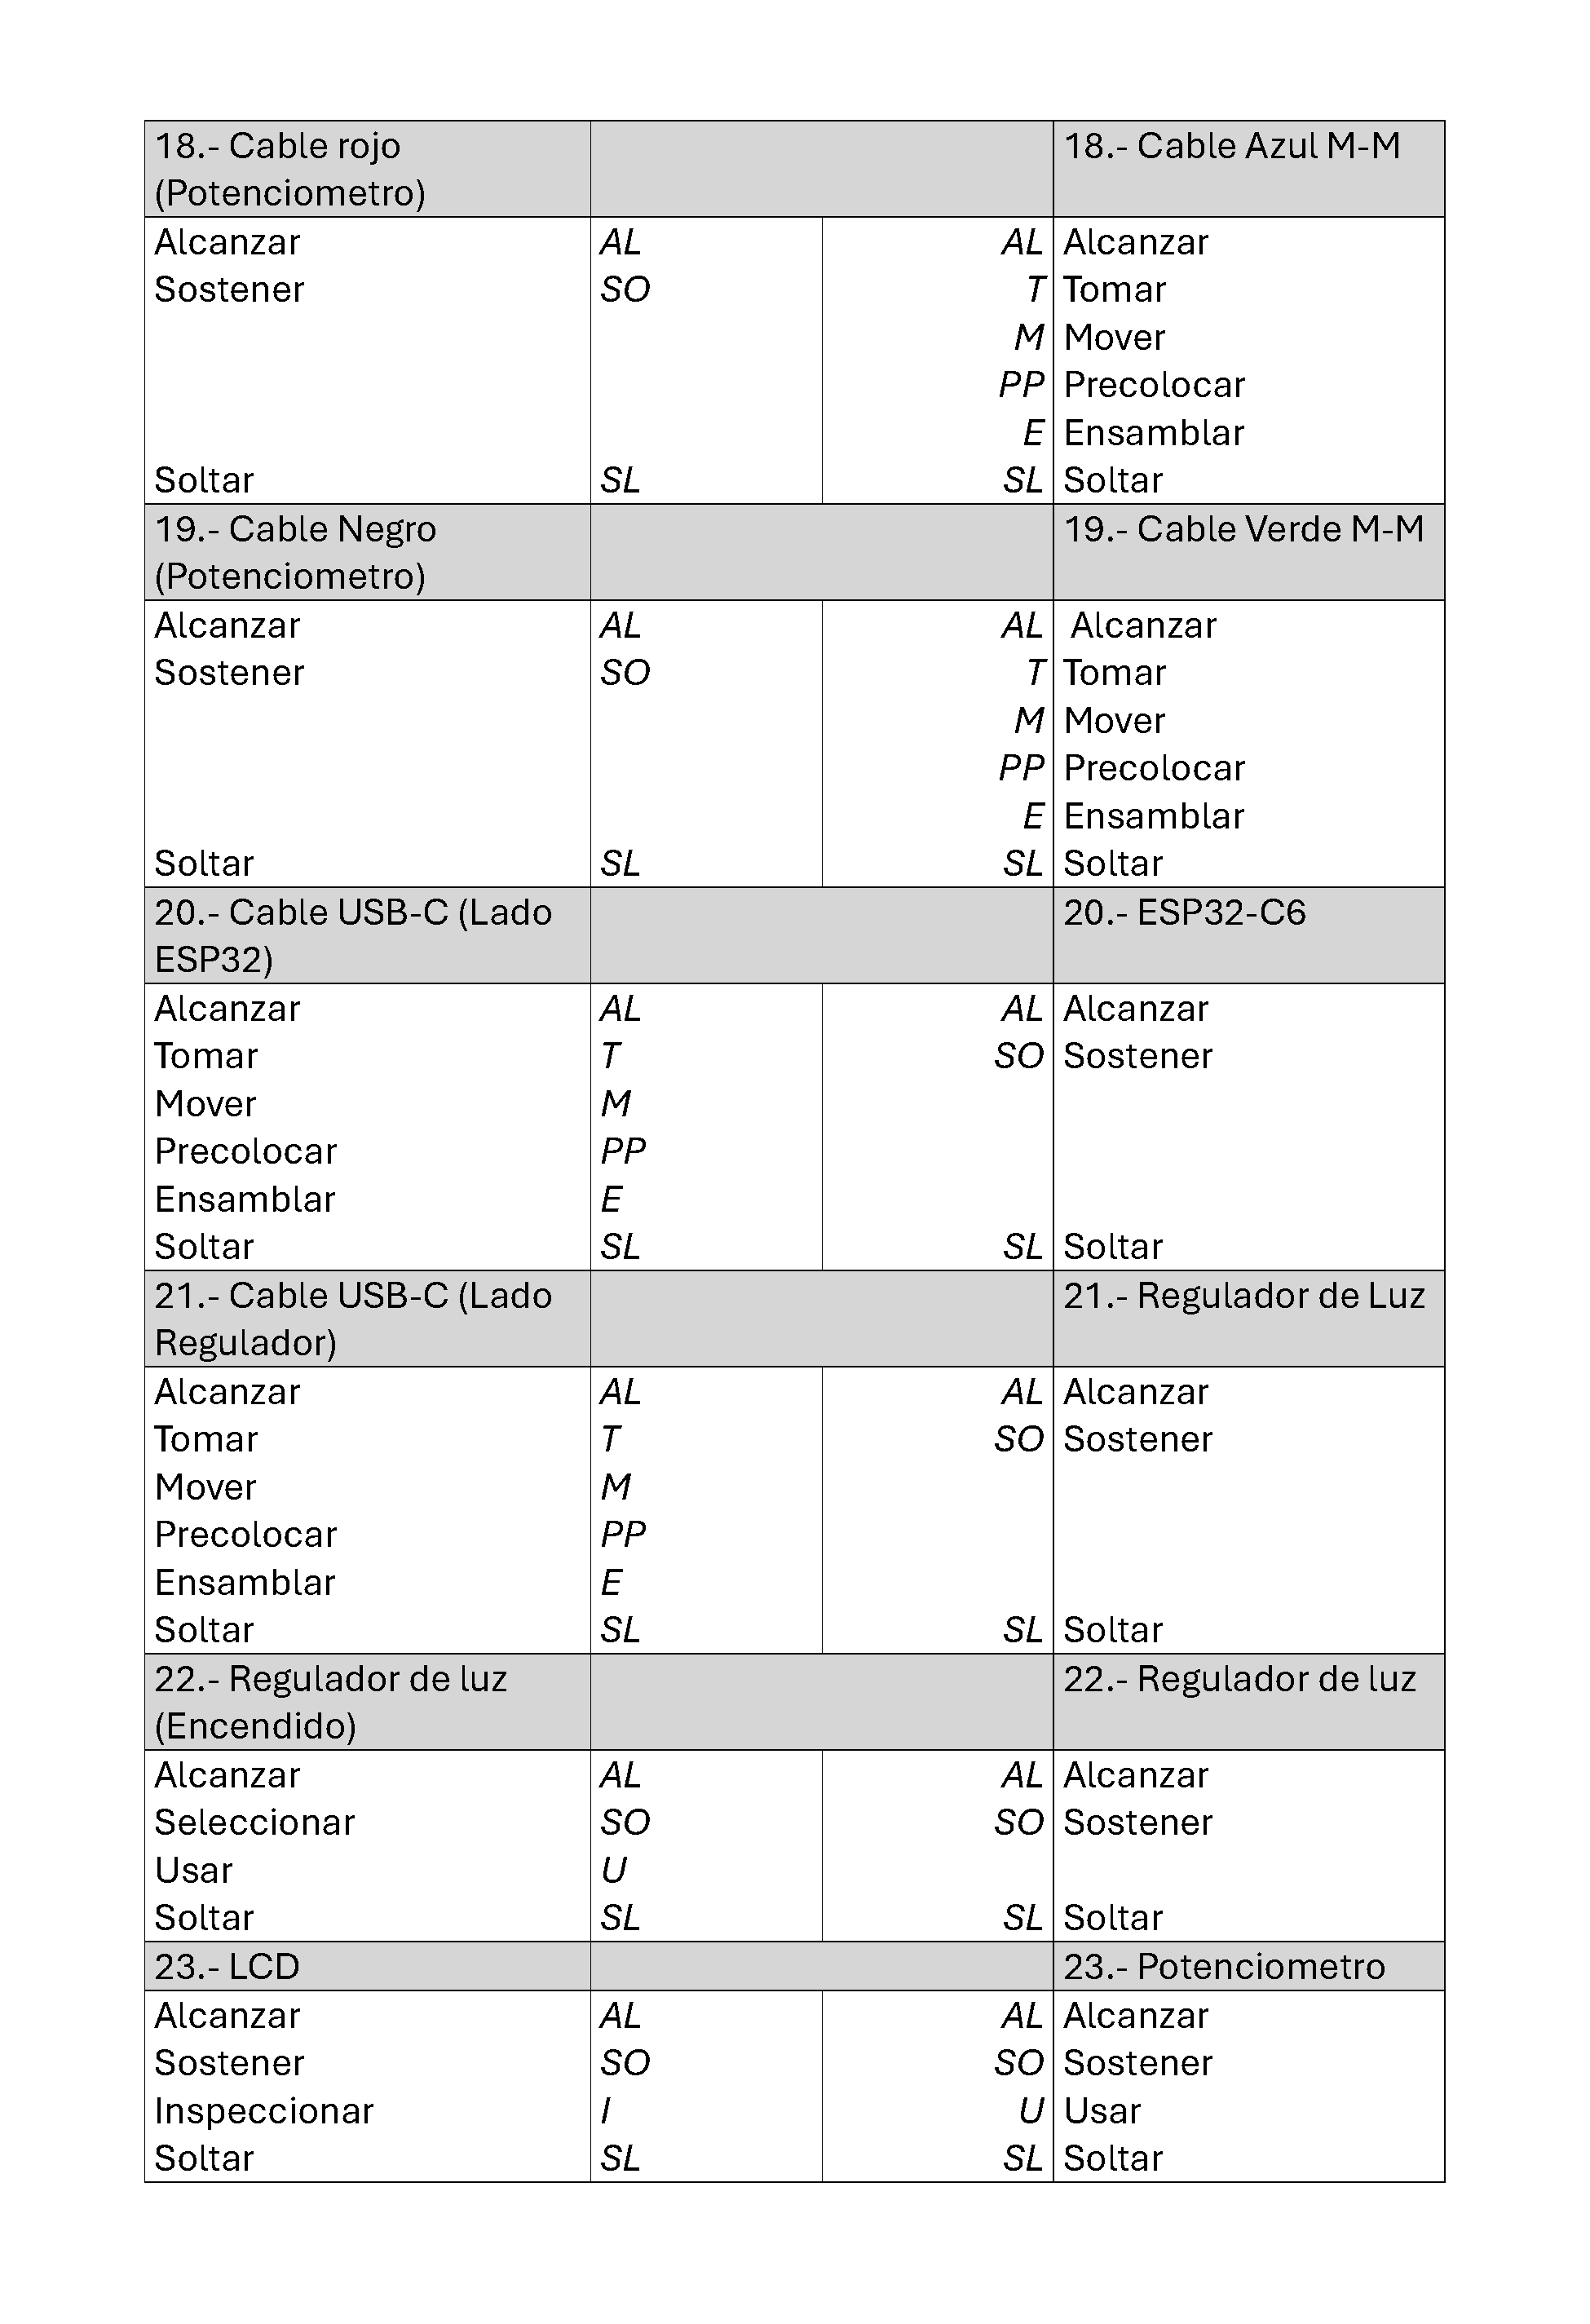
\includegraphics[scale=0.25]{30/img/diagramaBimanualEnsamble-4.pdf}
        \caption{Diagrama Bimanual}
        % \label{fig:my_label}
    \end{figure}
    % 
    % 
    \section{Conclusiones}
    
    Al avanzar en la práctica, se cubrieron diversos aspectos de las unidades de estudio de este curso, dado que este proyecto englobó todos los temas abordados a lo largo del semestre. Mayormente, se puede afirmar que se validó la hipótesis en un 70 por ciento, puesto que se consiguió mejorar las destrezas del estudiante, fortaleciendo así su habilidad para llevar a cabo nuevas prácticas y la aplicación de su conocimiento en la determinación del tiempo estándar de una tarea. De igual manera, se logró poner en marcha el plan de contingencia, donde se trataron varios puntos cruciales para la implementación de nuestra producción, como la identificación de riesgos internos y externos, la ubicación y los planos del instituto, y la identificación de recursos externos en caso de necesidad, incluyendo la recopilación de números telefónicos para cualquier eventualidad. Además, se llevó a cabo un análisis de métodos mediante la creación de nuestro propio manual, donde se examinaron los distintos procedimientos implicados. Esto abarcó la medición de materiales, la elaboración de esquemas, la identificación de componentes clave y una investigación exhaustiva de cada uno de estos elementos. Respecto a las herramientas, se determinó su uso específico para llevar a cabo el ensamblaje y se realizaron mediciones de las instalaciones del edificio, del salón y de la escuela. Con todo esto, se logró obtener una visión más integral de todo lo que conlleva llevar a cabo esta operación..
    
    \section{Agradecimientos}
    
    Es importante darles su debido reconocimiento a los laboratorios, instituciones, organizaciones, entre otros que han sido participes para la culminación de este trabajo. También es importante mencionar, fondos, proyectos, becas, entre otros que se le han otorgado al o los autores para realizar el trabajo de investigación. Ejemplo: “Los autores agradecen al Concejo Nacional de Ciencia y Tecnología por los recursos otorgados…”
    
    % \section*{Referencias}
    
    % Para esta platilla, se solicita al autor enumerar las citas de manera consecutiva entre corchetes \cite{YLi2013}. 
    % La puntuación de la oración que sigues sería \cite{Mesaelides2011}. 
    % Refiérase simplemente al número de referencia, como en \cite{Morales2012}, no utilice “Ref. [3]” o “referencia [3]” excepto al principio de una oración: “La referencia [3] fue la primera…”
    % Enumere las notas al pie por separado en superíndices. Coloque la nota de pie de en la parte inferior de la columna en la que se citó. No coloque notas al pie en la lista de referencias. Utilice letras para las notas al pie de la tabla.
    % A menos de que haya tres autores o más; no utilice “et al.”. Los trabajos que no hayan sido publicados, incluso si han sido presentados para su publicación, deben ser citados como “inéditos”. Los trabajos que han sido aceptados para su publicación deben de citarse como “en prensa”. Poner en mayúscula sólo la primera palabra de un título, excepto los nombres propios y los símbolos de elemento. 
    % Otros ejemplos \cite{LAAngeles2021}, \cite{LAAngelesConni}. 
    % Véase el link \cite{prueba}, Véase el Apéndice \ref{anexo:pines}.
    
    % Ejemplo
    %  @Article{article,
    % 	author = "Author1 LastName1 and Author2 LastName2 and Author3 LastName3",
    % 	title = "Article Title",
    % 	volume = "30",
    % 	number = "30",
    % 	pages = "10127-10134",
    % 	year = "2013",
    % 	doi = "10.3389/fnins.2013.12345",
    % 	URL = "http://www.frontiersin.org/Journal/10.3389/fnins.2013.12345/abstract",
    % 	journal = "Frontiers in Neuroscience"
    % }
    
    % @book{book,
    %   author    = {Author Name}, 
    %   title     = {The title of the work},
    %   publisher = {The name of the publisher},
    %   address   = {The city},
    %   year      = 1993,
    % }
    
    % @incollection{chapter,
    %   author       = {Bauthor Surname}, 
    %   title        = {The title of the work},
    %   editor       = {Editor Name},
    %   booktitle    = {The title of the book},
    %   publisher    = {The name of the publisher},
    %   address      = {The city},
    %   year         = 2002,
    %   pages        = {201-213},
    % }
    
    % @InProceedings{conference,
    %   author = {Cauthor Name and Dauthor Surname and Fauthor LastName},
    %   title = {The title of the work},
    %   booktitle = {The title of the conference proceedings},
    %   year = 1996,
    %   publisher = {The name of the publisher},
    %   editor = {Editor Name1 and Editor Name2},
    %   pages = {41-50},
    % }
    
    % @book{cho,
    %   author       = {Gauthor Name1}, 
    %   title        = {The title of the work},
    %   publisher = {Country code and patent number},
    %   address      = {Patent Country},
    %   year = 2013
    % }
    
    % @book{patent,
    %   author    = {Hauthor Surname1}, 
    %   title     = {The title of the work},
    %   publisher = {Patent number},
    %   address   = {Patent country},
    %   year      = 2010,
    % }
    
    % % please use misc for datasets
    % @misc{dataset, 
    % 	author = "Author1 LastName1 and Author2 LastName2 and Author3 LastName3",
    % 	title = "Data Title",
    % 	year = "2011",
    % 	doi = "10.000/55555",
    % 	URL = "http://www.frontiersin.org/",
    % }
    
    \bibliographystyle{ieeetr}
    \bibliography{30/referencias}
    % 
    % 
    %%%%%%%%%%%%%%%%%%%%%%%%%%%%%%%%%%
    \appendix
    %%%%%%%%%%%%%%%%%%%%%%%%%%%%%%%%%%
    % 
    % 
    % \centering{\section[\appendixautorefname{}]{Apéndice}}\label{anexo:pines}
    % \includepdf[pages=-]{6/Img/pines.pdf}
    %%%%%%%%%%%%%%%%%%%%%%%%%%%%%%%%%%%%%%%%